\documentclass[a4paper,12pt]{article}

\usepackage{../usfdvl}


\title{Worksheet 3}
\SetDocumentFooter{}{}


\begin{document}

\maketitle

\worksheetGroundRules


\vspace{5pt}
\section{Assignment}

\begin{enumerate}


\item For the following polygon (you can use the large image on the next page):

\begin{minipage}[m]{0.6\textwidth}
\begin{itemize}
\item Draw all possible edges between non-adjacent vertices. 
\item Denote those segments which are diagonals and those which are not. 
\item For non-diagonal segments, state the reason they are not considered diagonal. 
\item Is the polygon convex? Why or why not?
\end{itemize}
\end{minipage}
%
\hfill
%
\begin{minipage}[m]{5.5cm}
\begin{center}
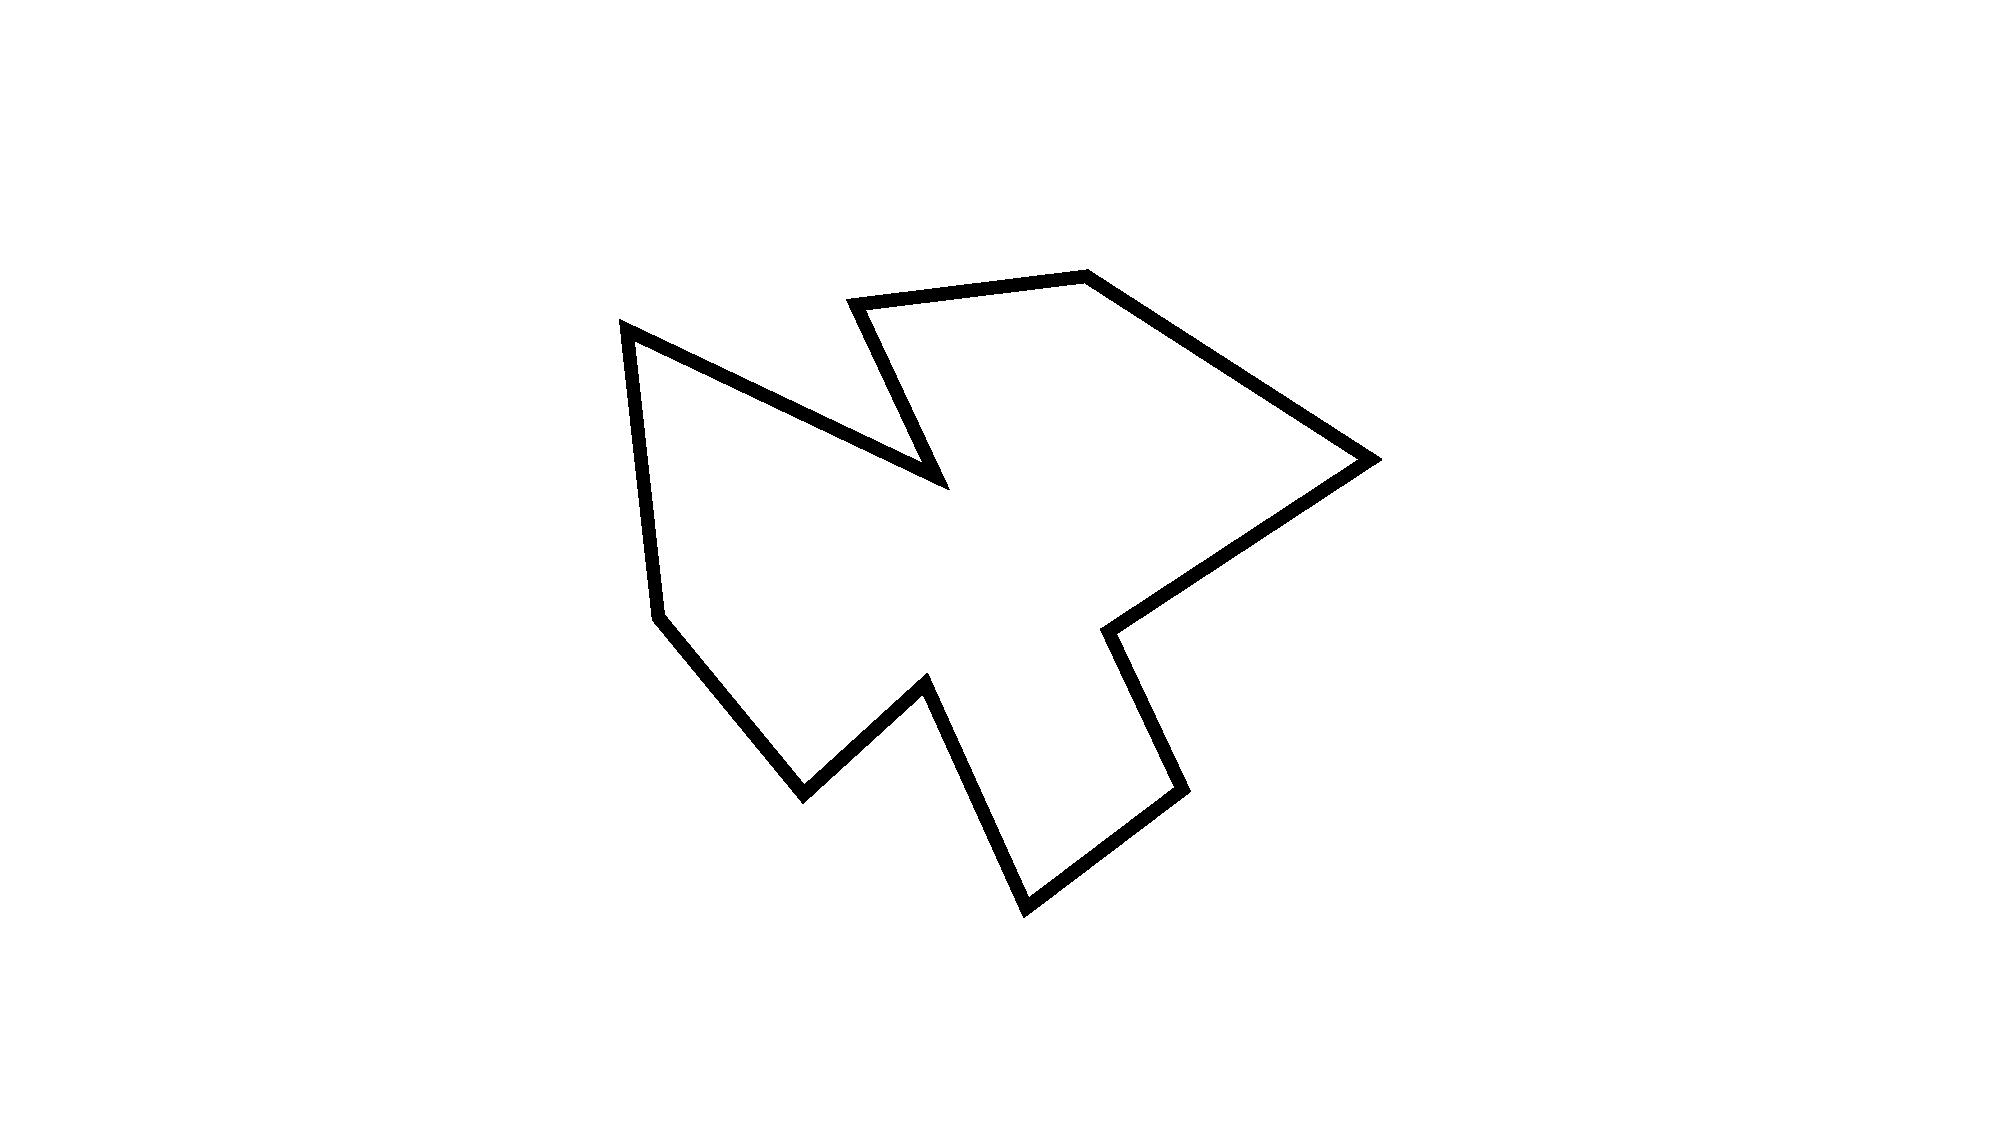
\includegraphics[width=5cm]{../images/worksheet2a.pdf}
\end{center}
\end{minipage}




\item Given the 2 convex polygons, $A$ and $B$, show the steps of the $O(M+N)$ algorithm to find $A \cap B$ discussed in class. Your algorithm should start at $a_0$ and $b_0$. (Use the page at the end of the document.)


\begin{center}
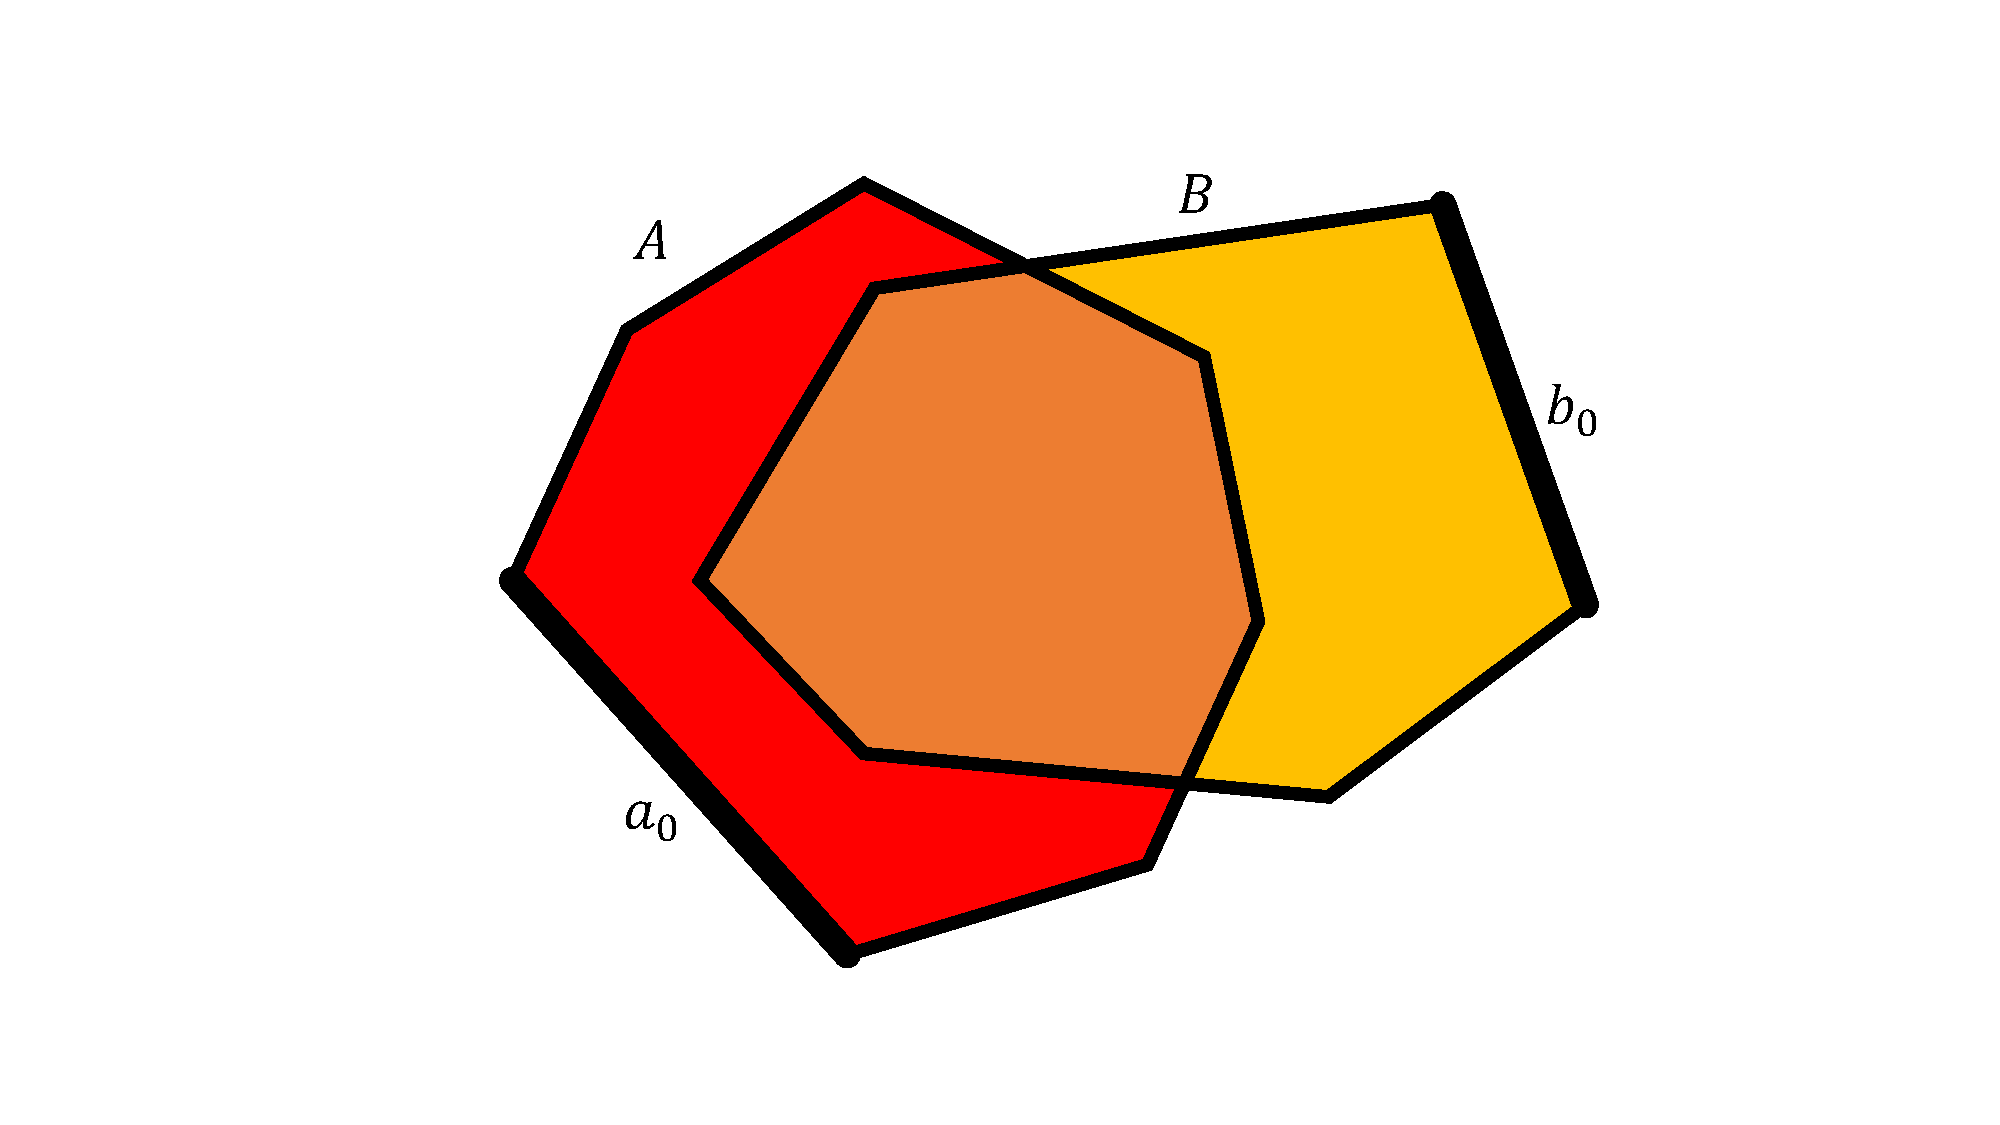
\includegraphics[width=5cm]{../images/worksheet2b.pdf}
\end{center}

\begin{itemize}
\item Describe how you would modify the algorithm to find $A \cup B$, $A \backslash B$, and $A \ominus B$. (hint: describe it in terms of inner and outer chains.)
\end{itemize}


\end{enumerate}

\worksheetSubmission


\newpage

\begin{center}
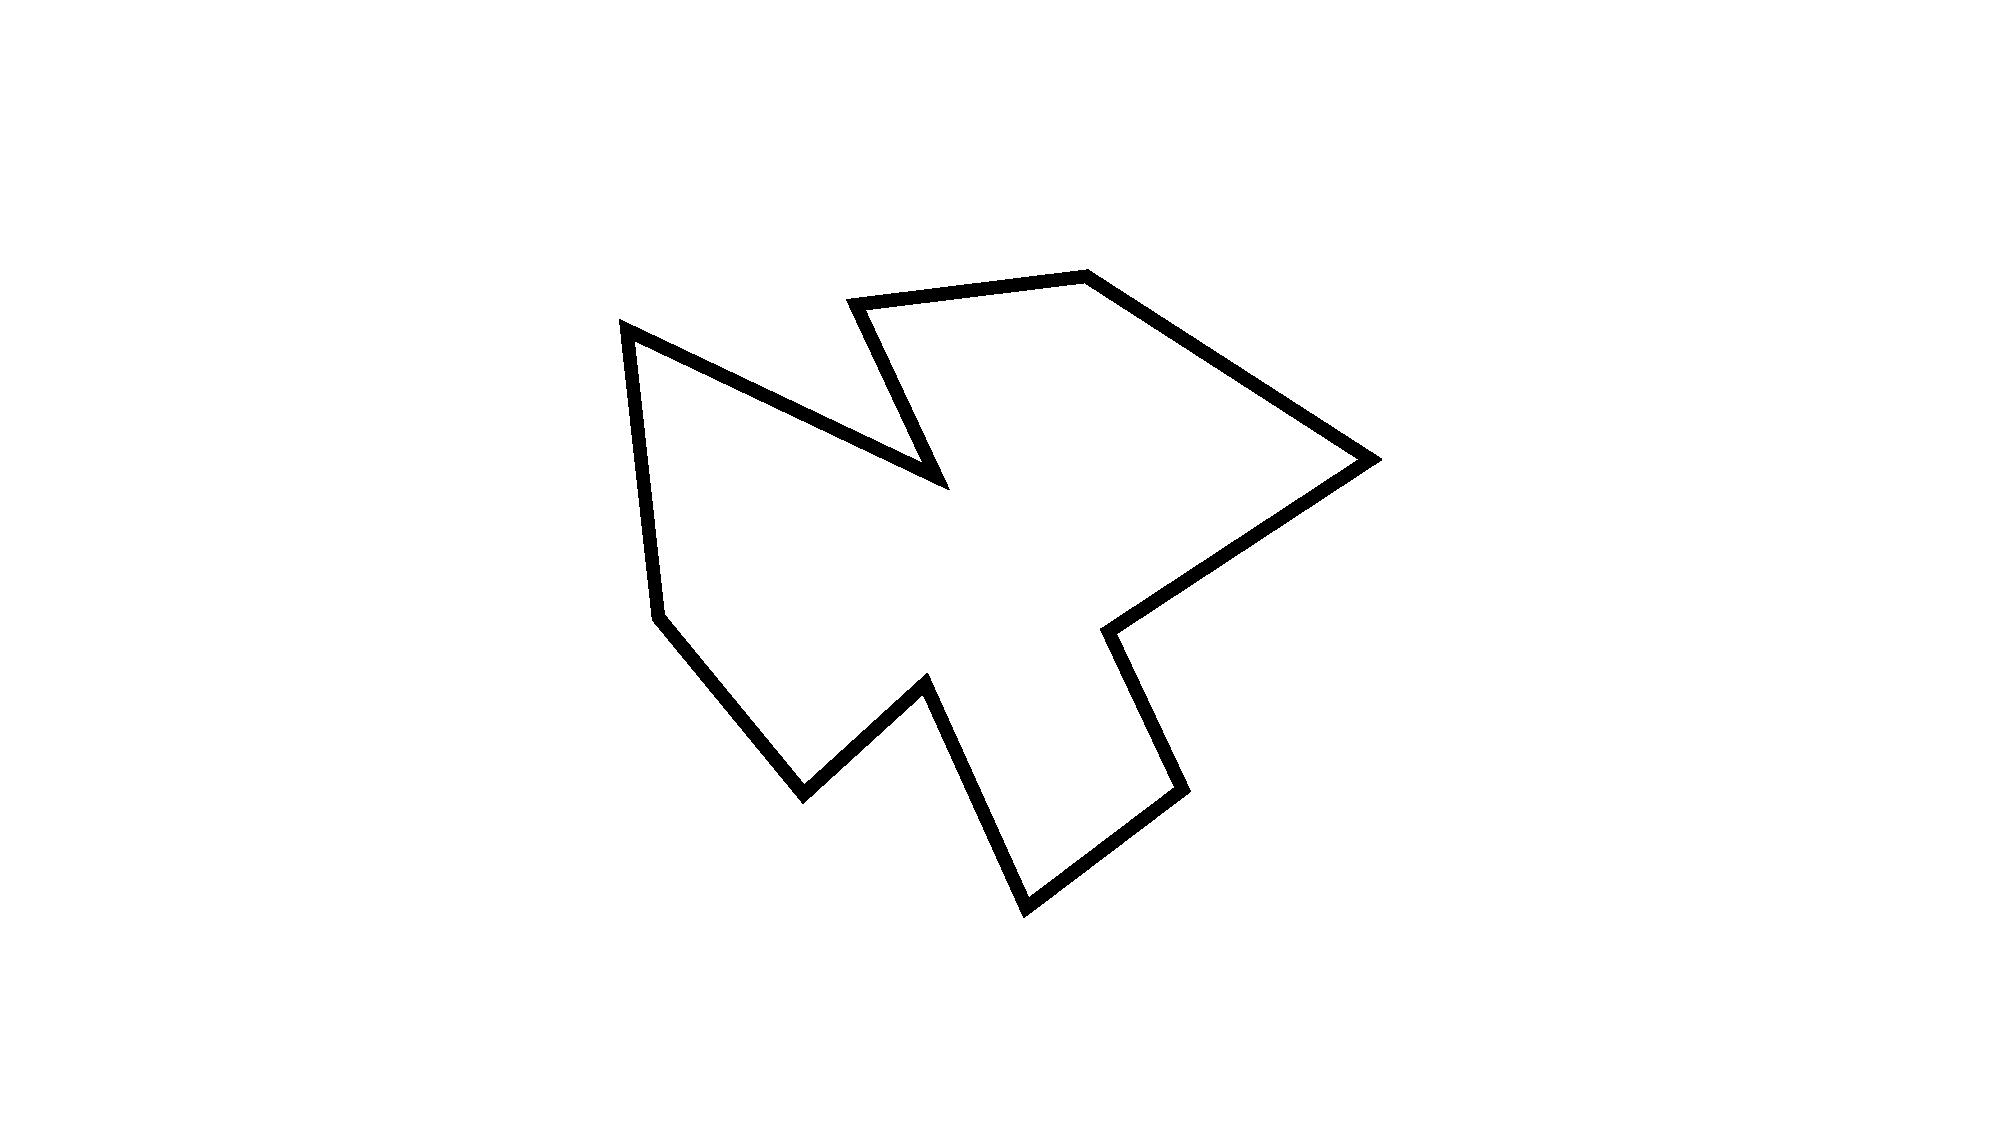
\includegraphics[width=0.8\linewidth]{../images/worksheet2a.pdf}
\end{center}

\newpage

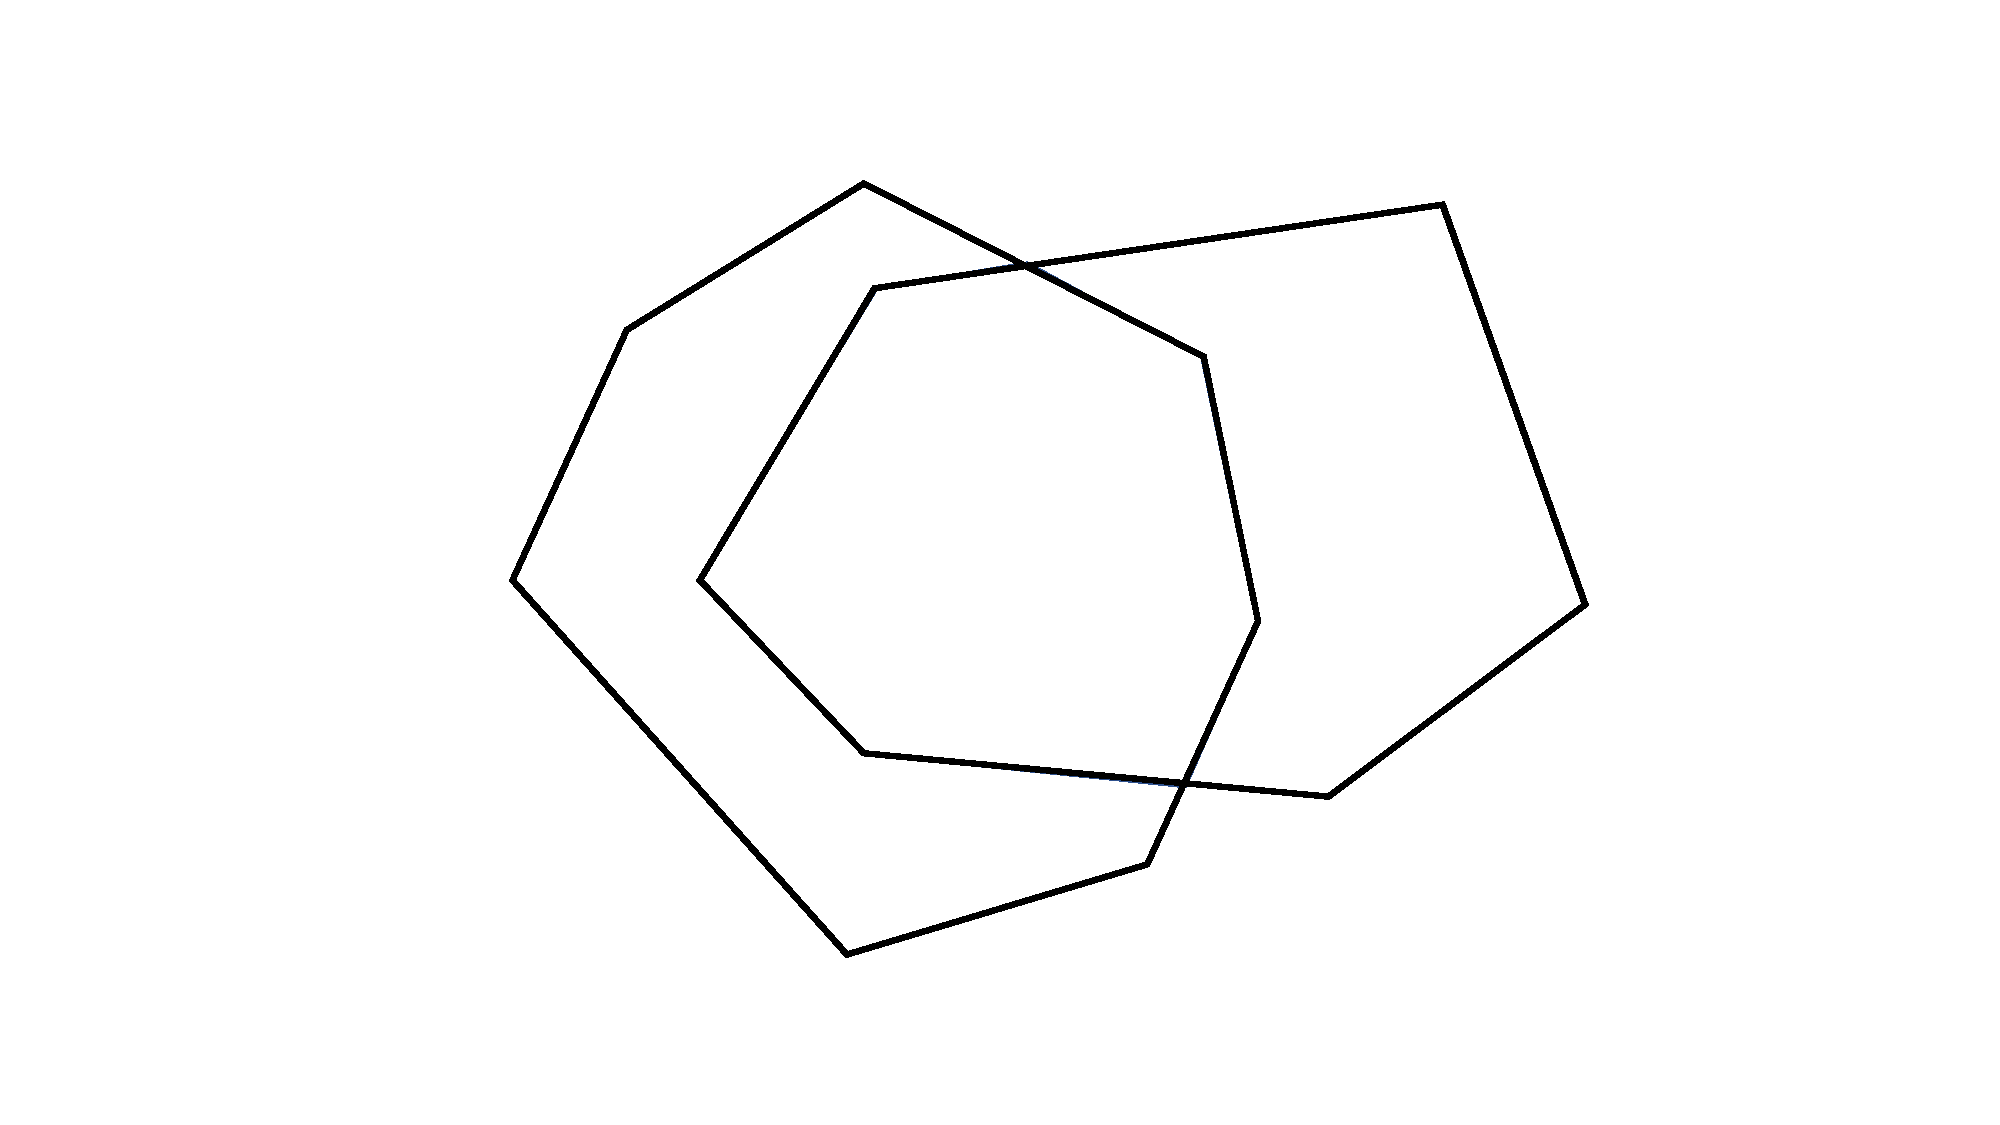
\includegraphics[width=0.3\linewidth]{../images/worksheet2b_no_color.pdf}\hfill
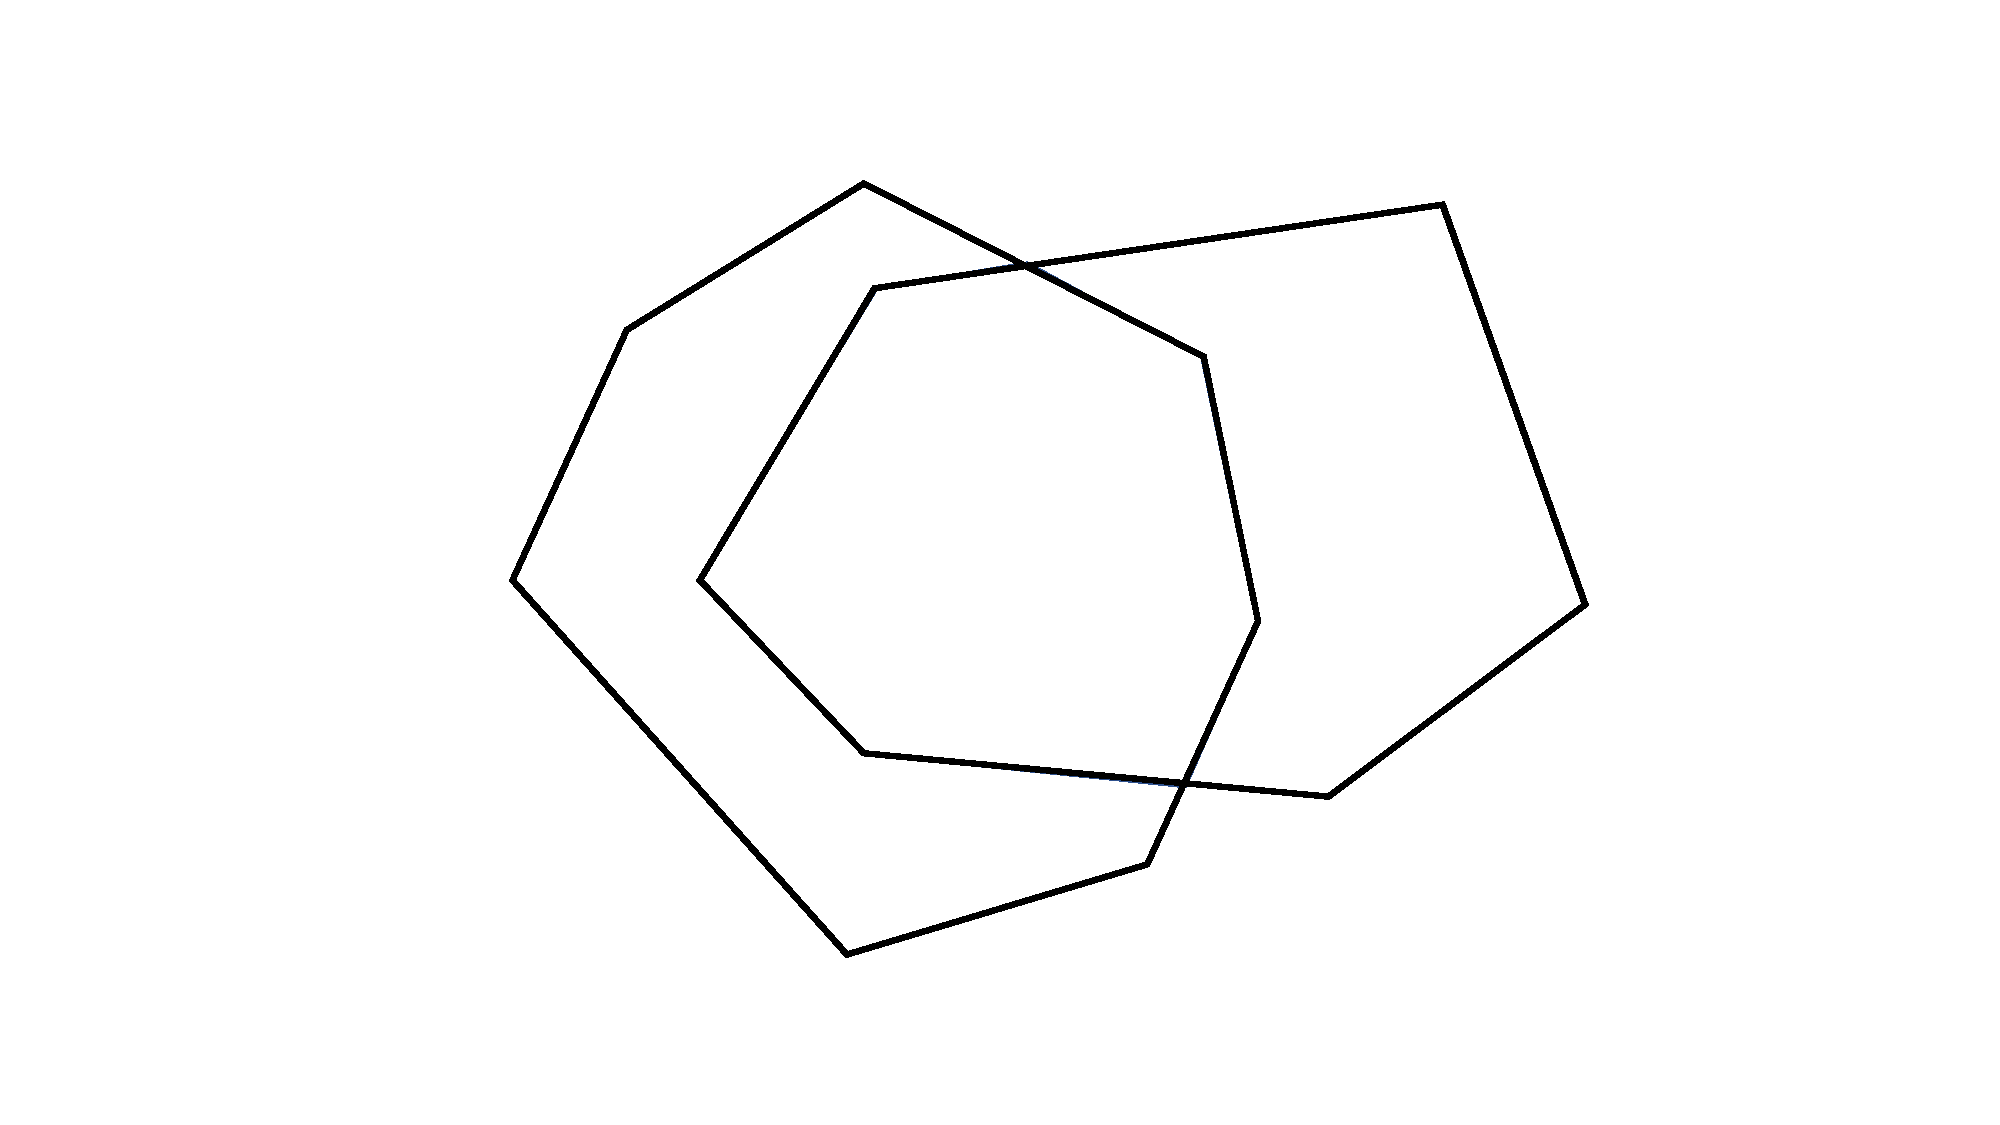
\includegraphics[width=0.3\linewidth]{../images/worksheet2b_no_color.pdf}\hfill
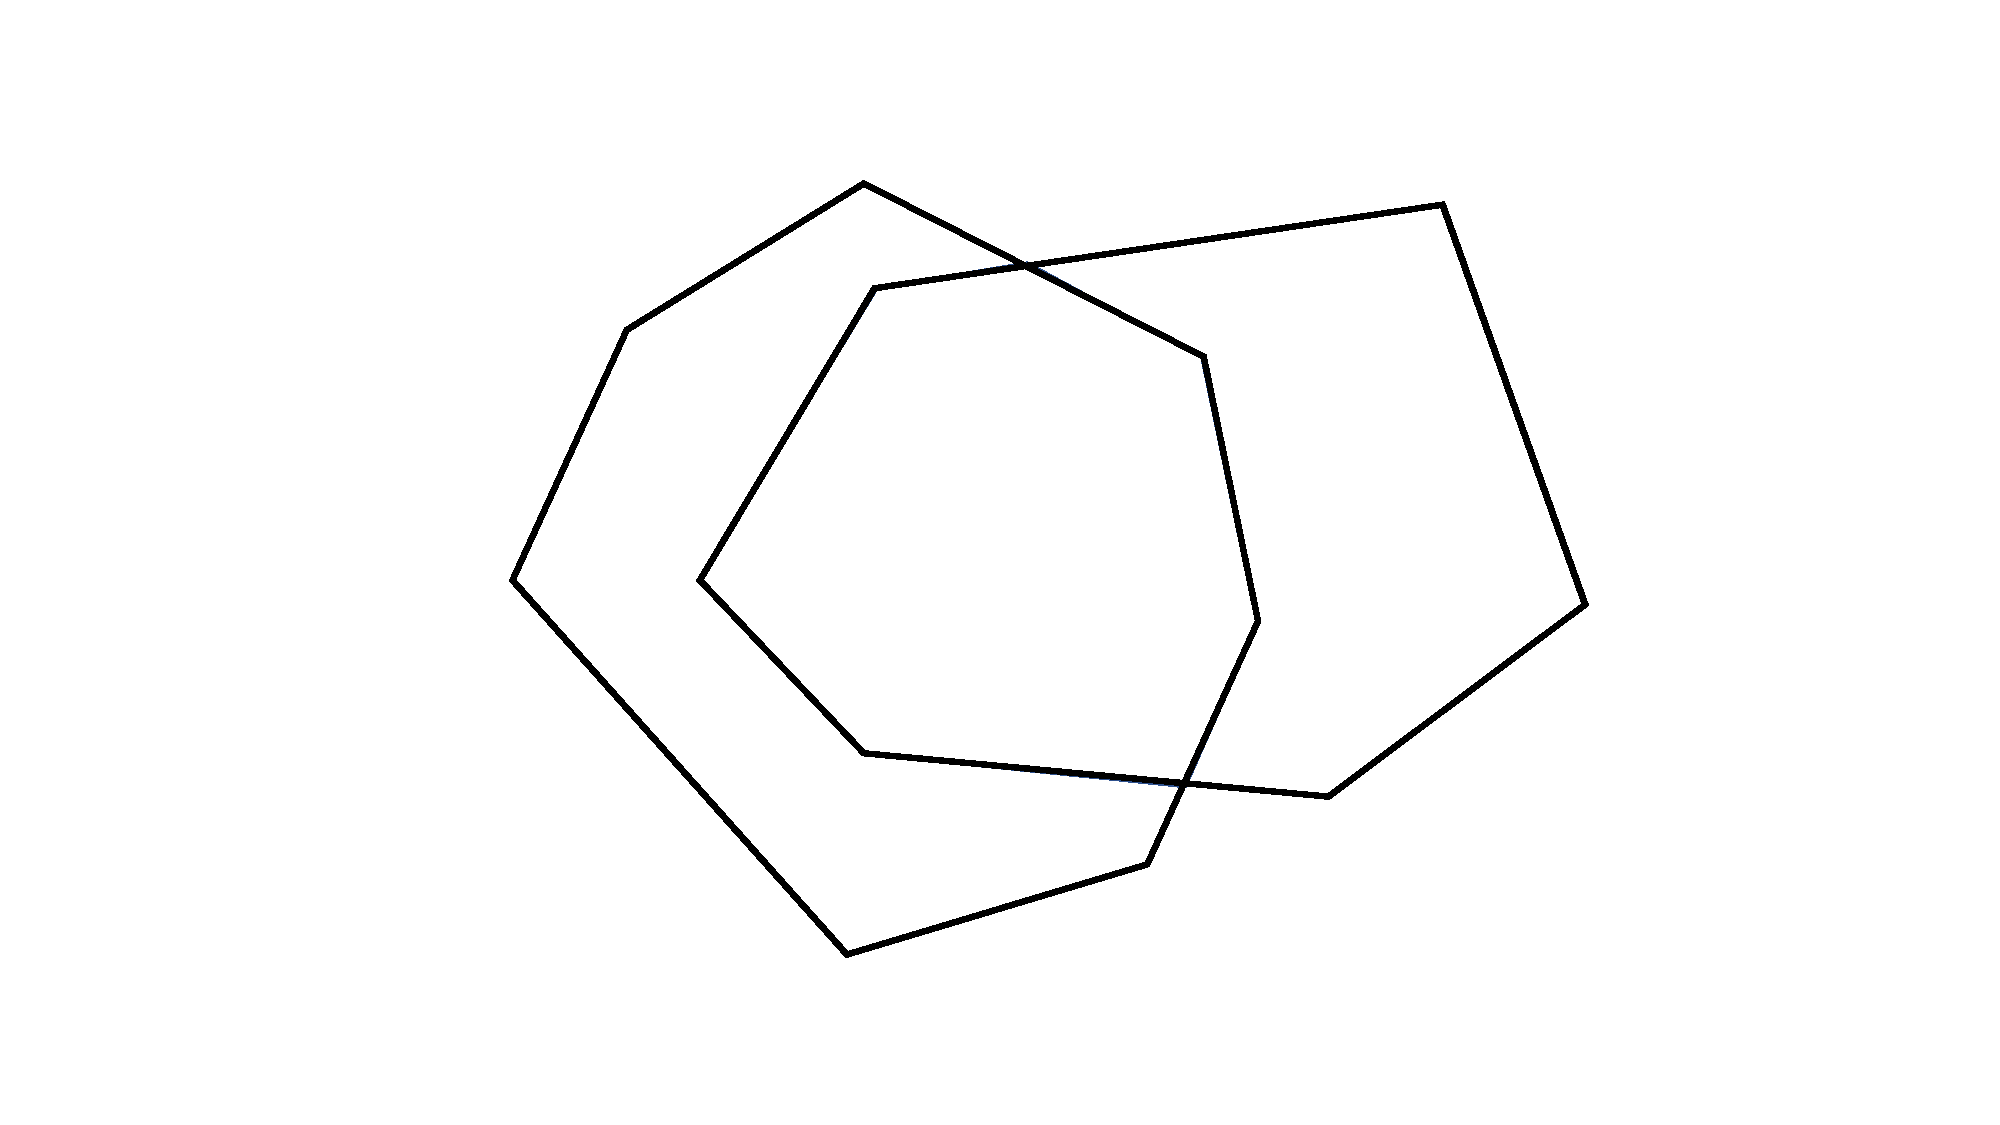
\includegraphics[width=0.3\linewidth]{../images/worksheet2b_no_color.pdf}

\vspace{25pt}
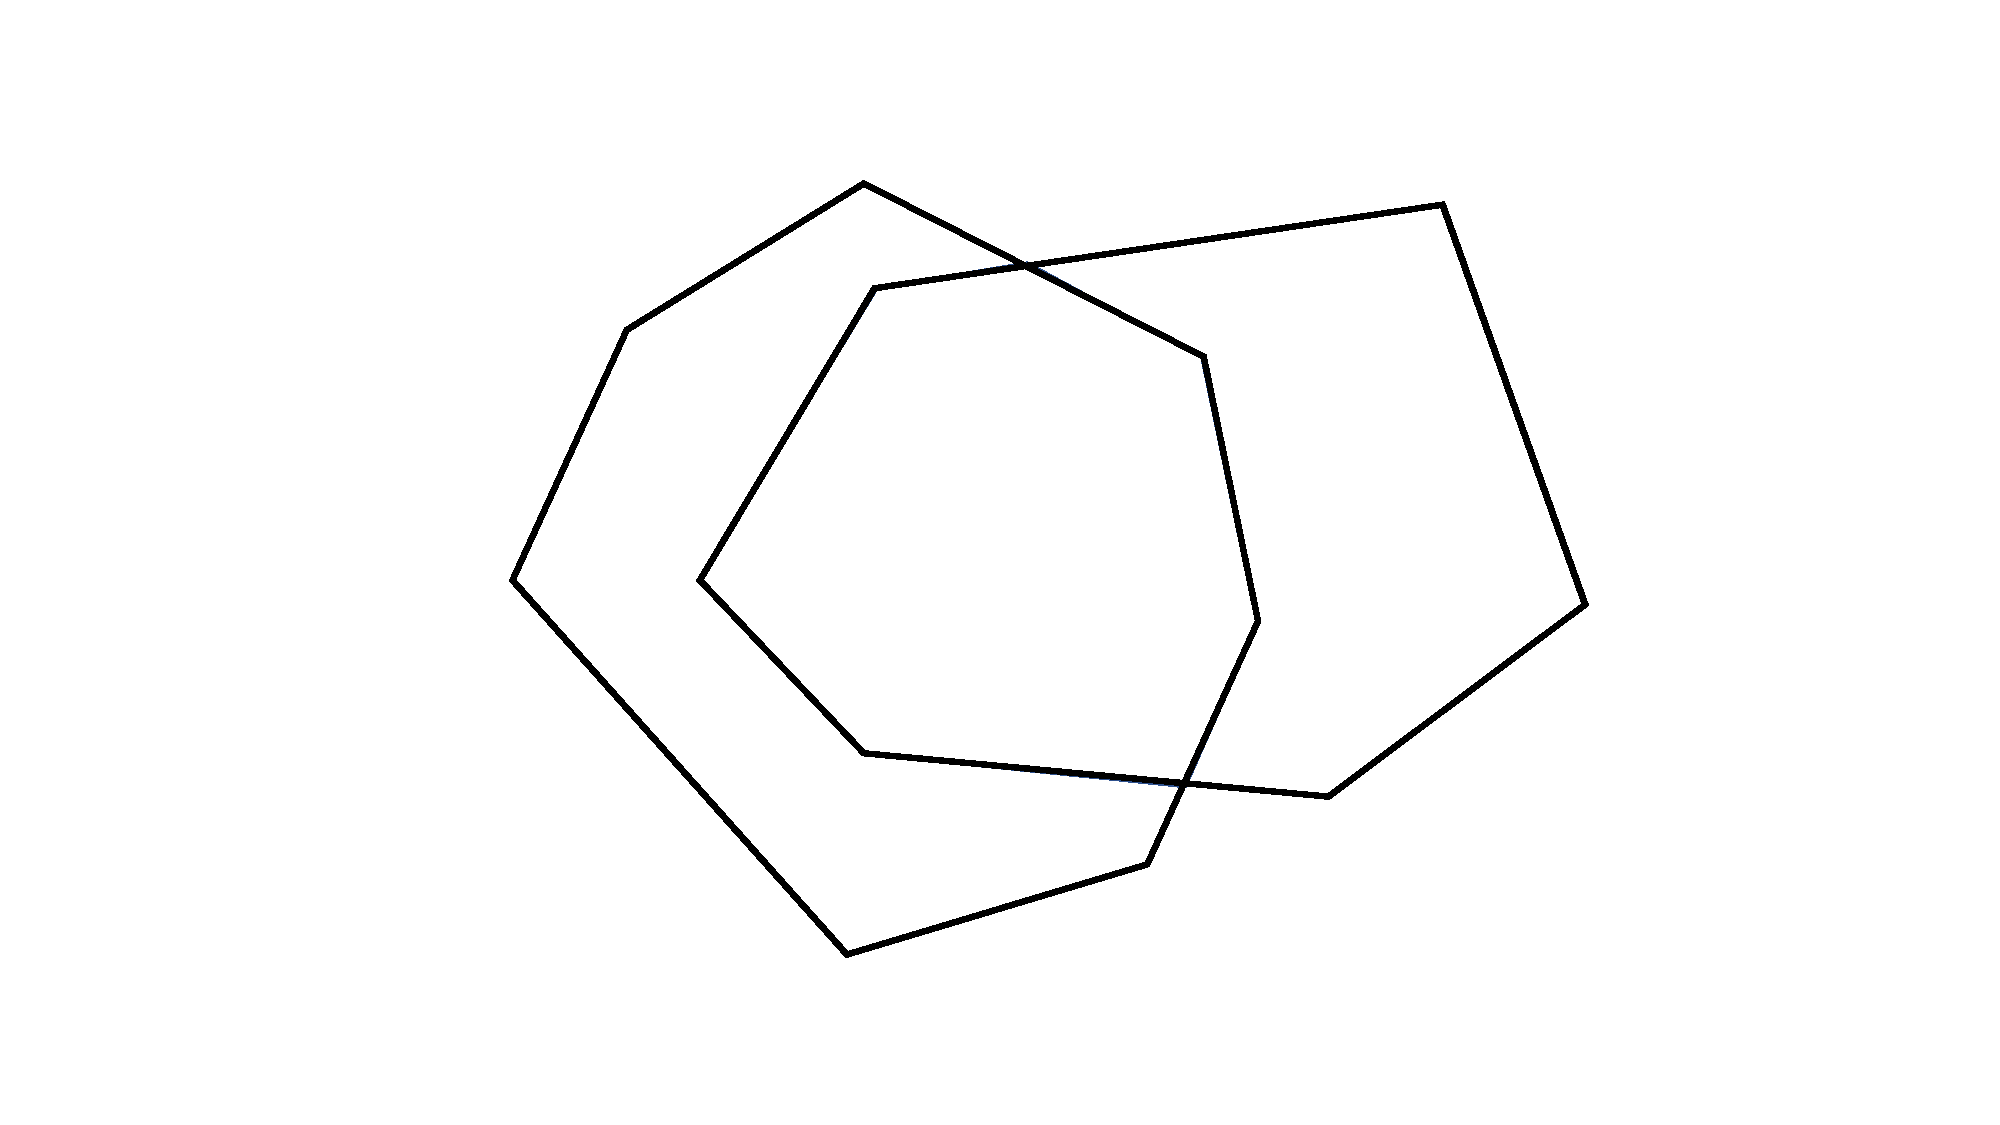
\includegraphics[width=0.3\linewidth]{../images/worksheet2b_no_color.pdf}\hfill
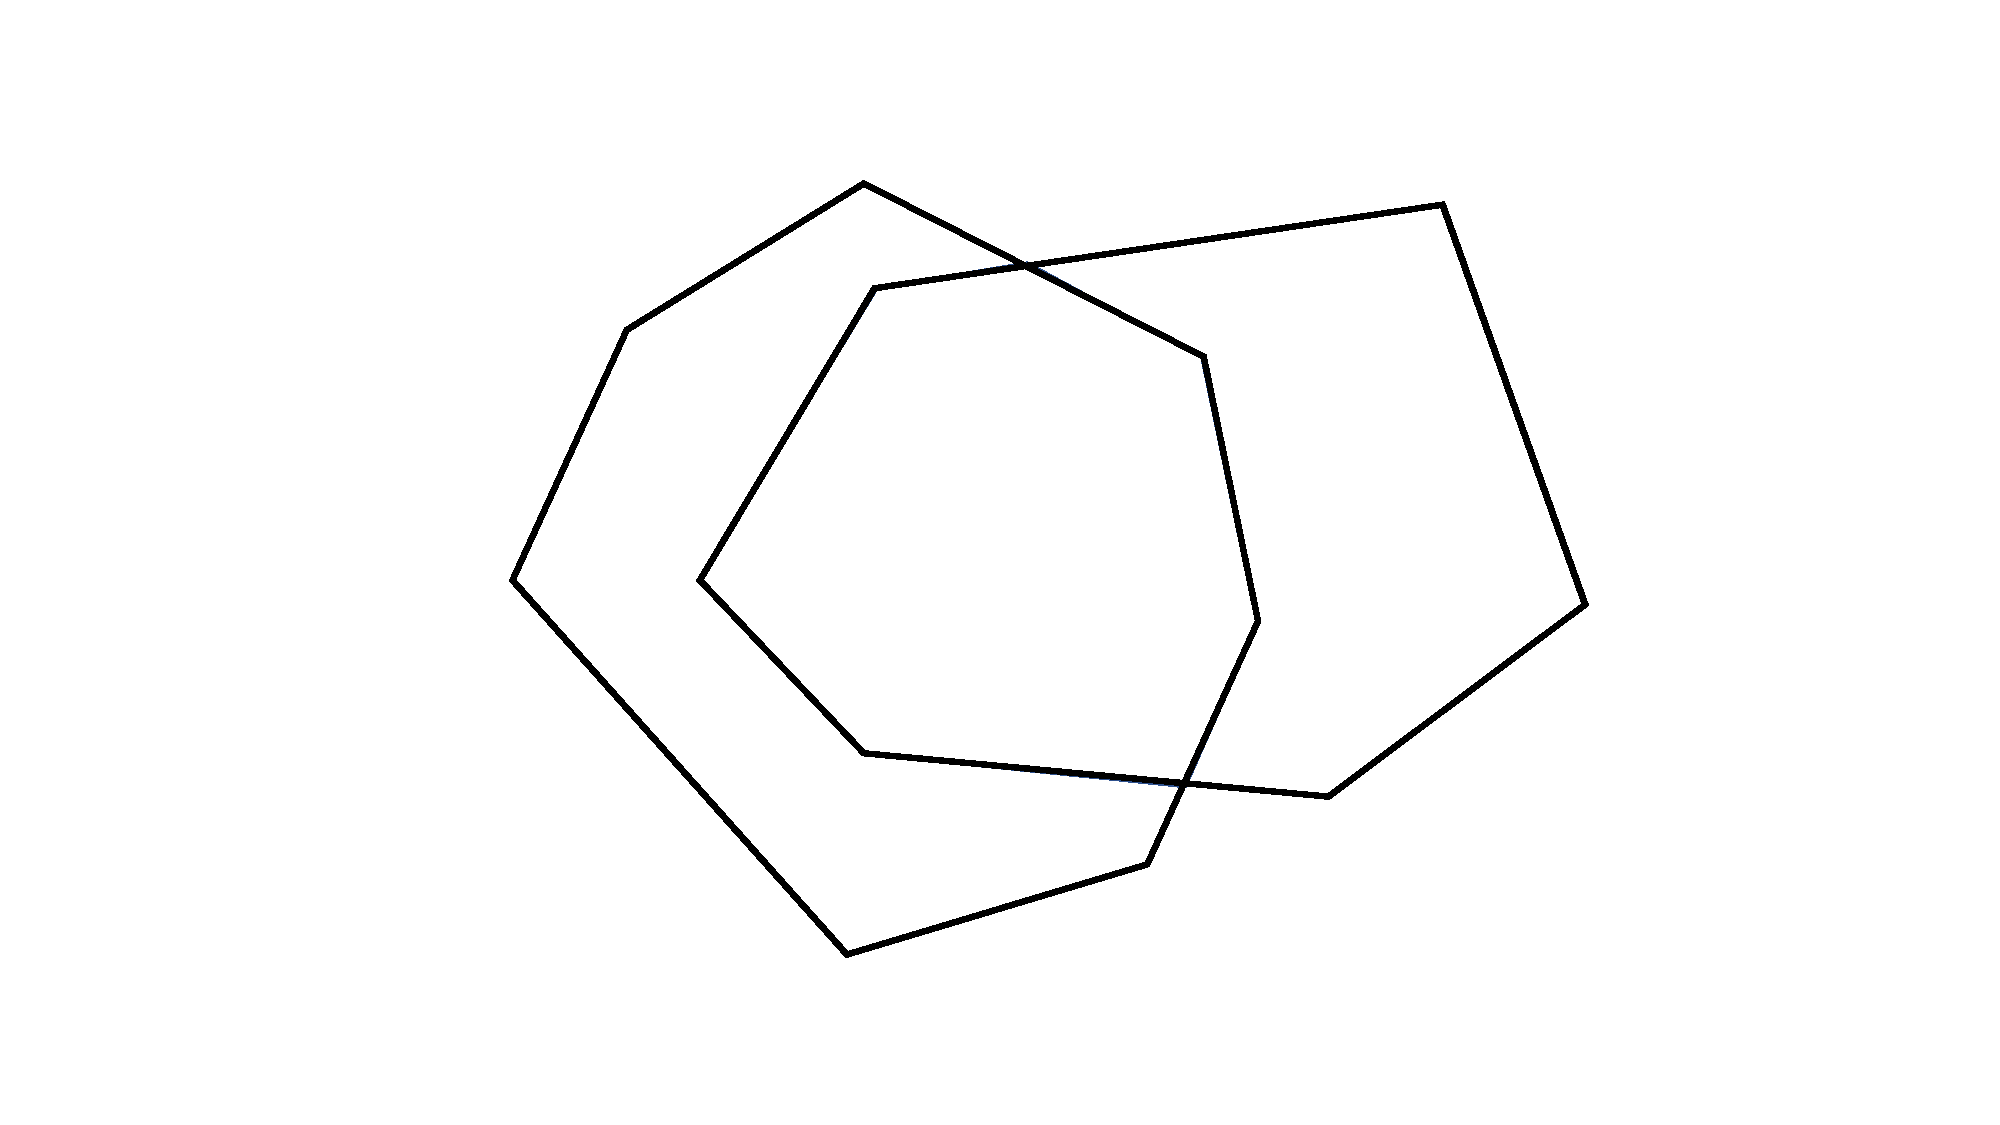
\includegraphics[width=0.3\linewidth]{../images/worksheet2b_no_color.pdf}\hfill
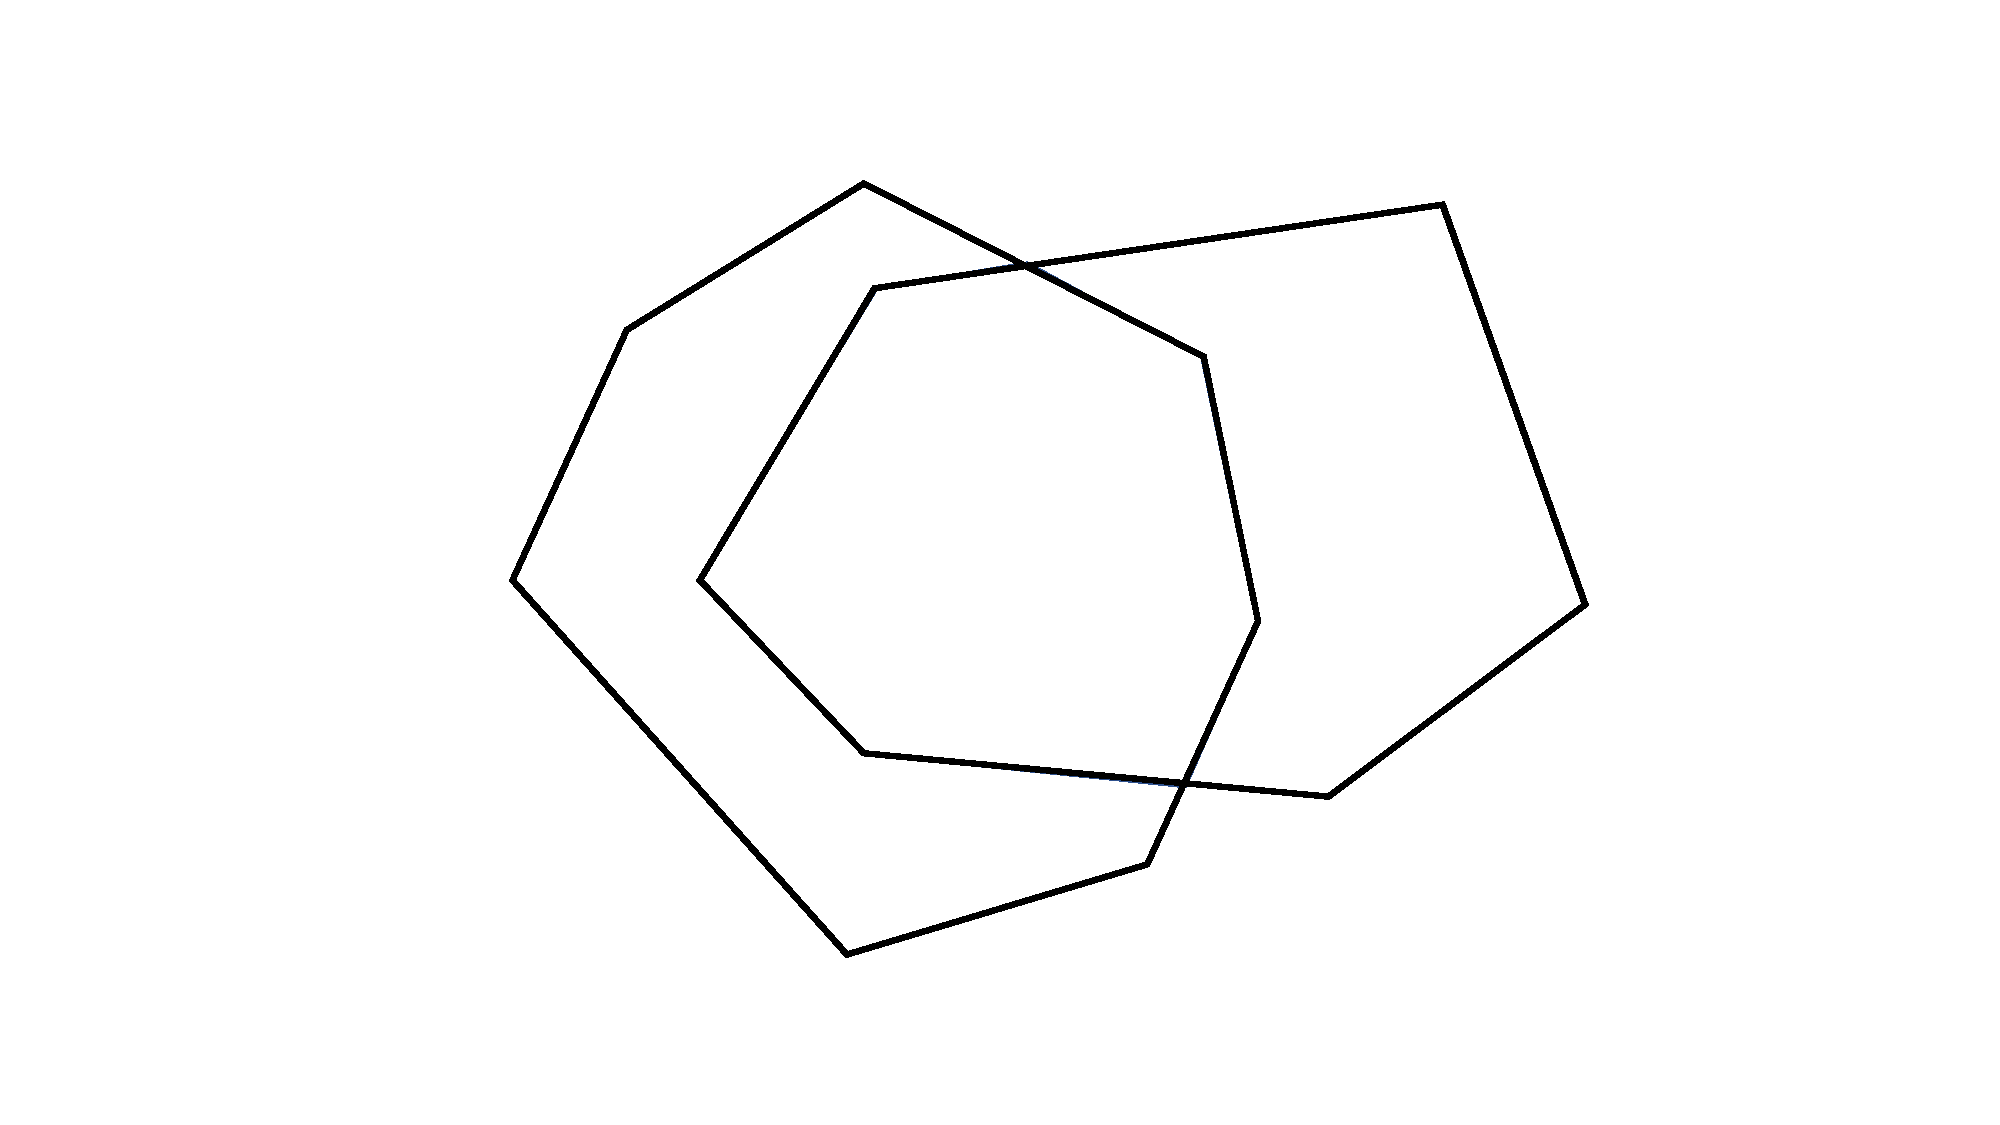
\includegraphics[width=0.3\linewidth]{../images/worksheet2b_no_color.pdf}

\vspace{25pt}
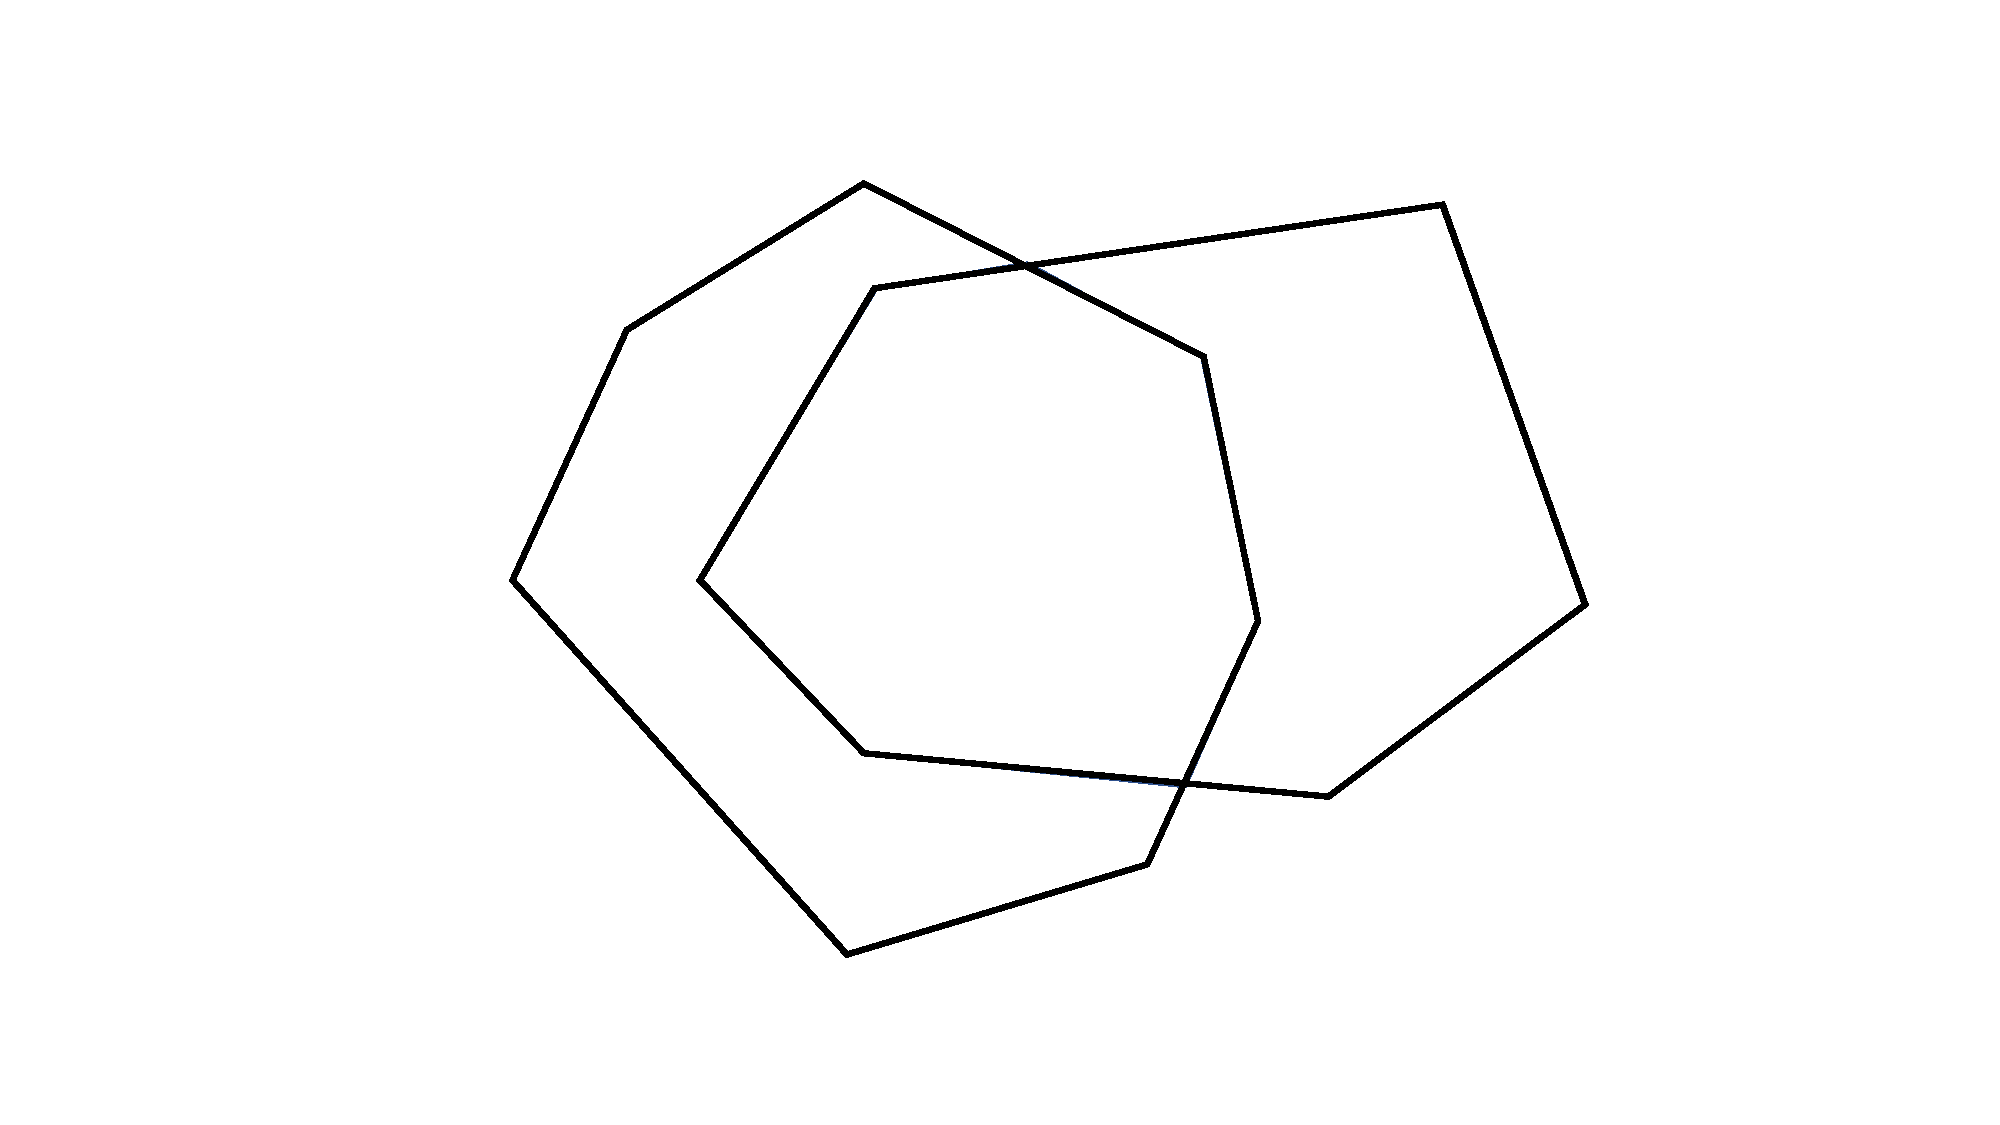
\includegraphics[width=0.3\linewidth]{../images/worksheet2b_no_color.pdf}\hfill
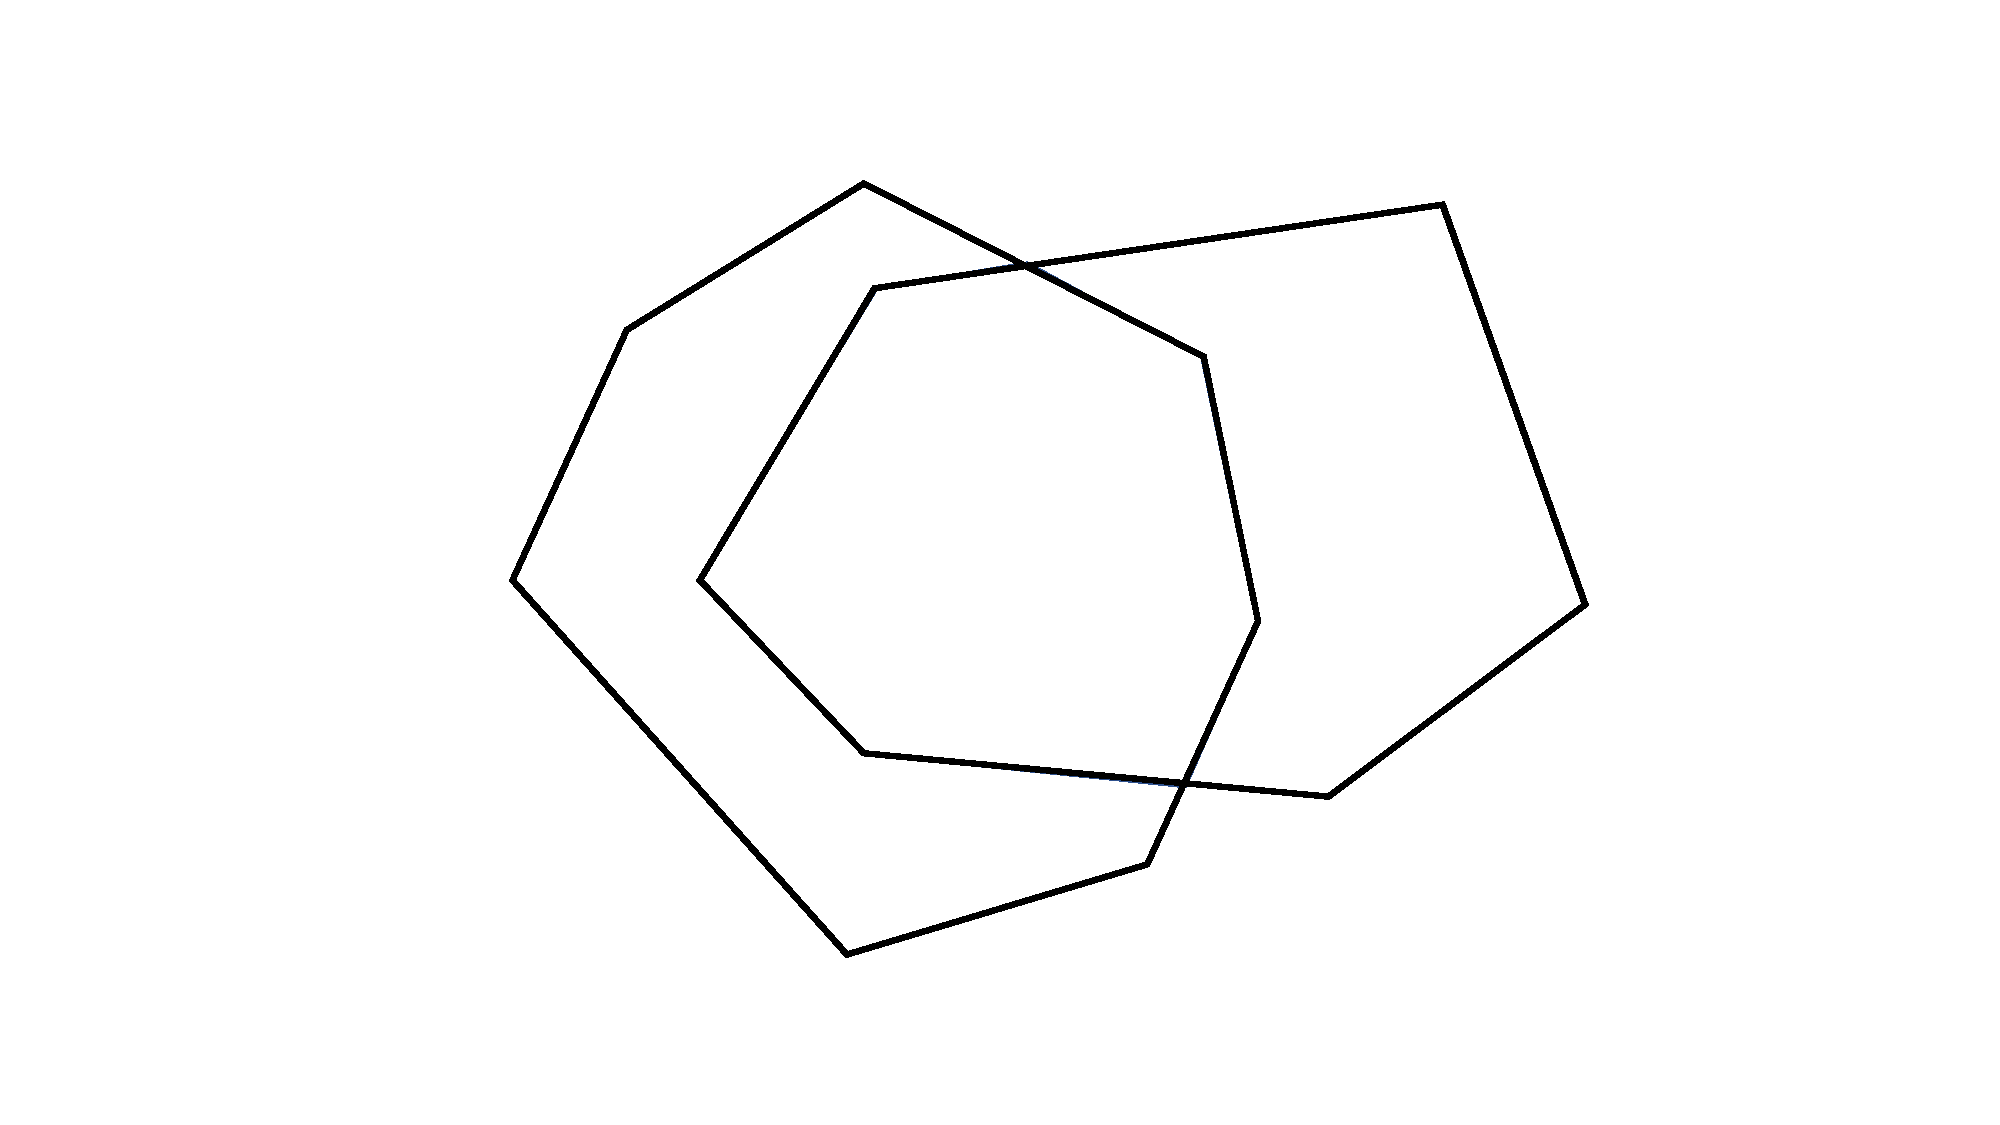
\includegraphics[width=0.3\linewidth]{../images/worksheet2b_no_color.pdf}\hfill
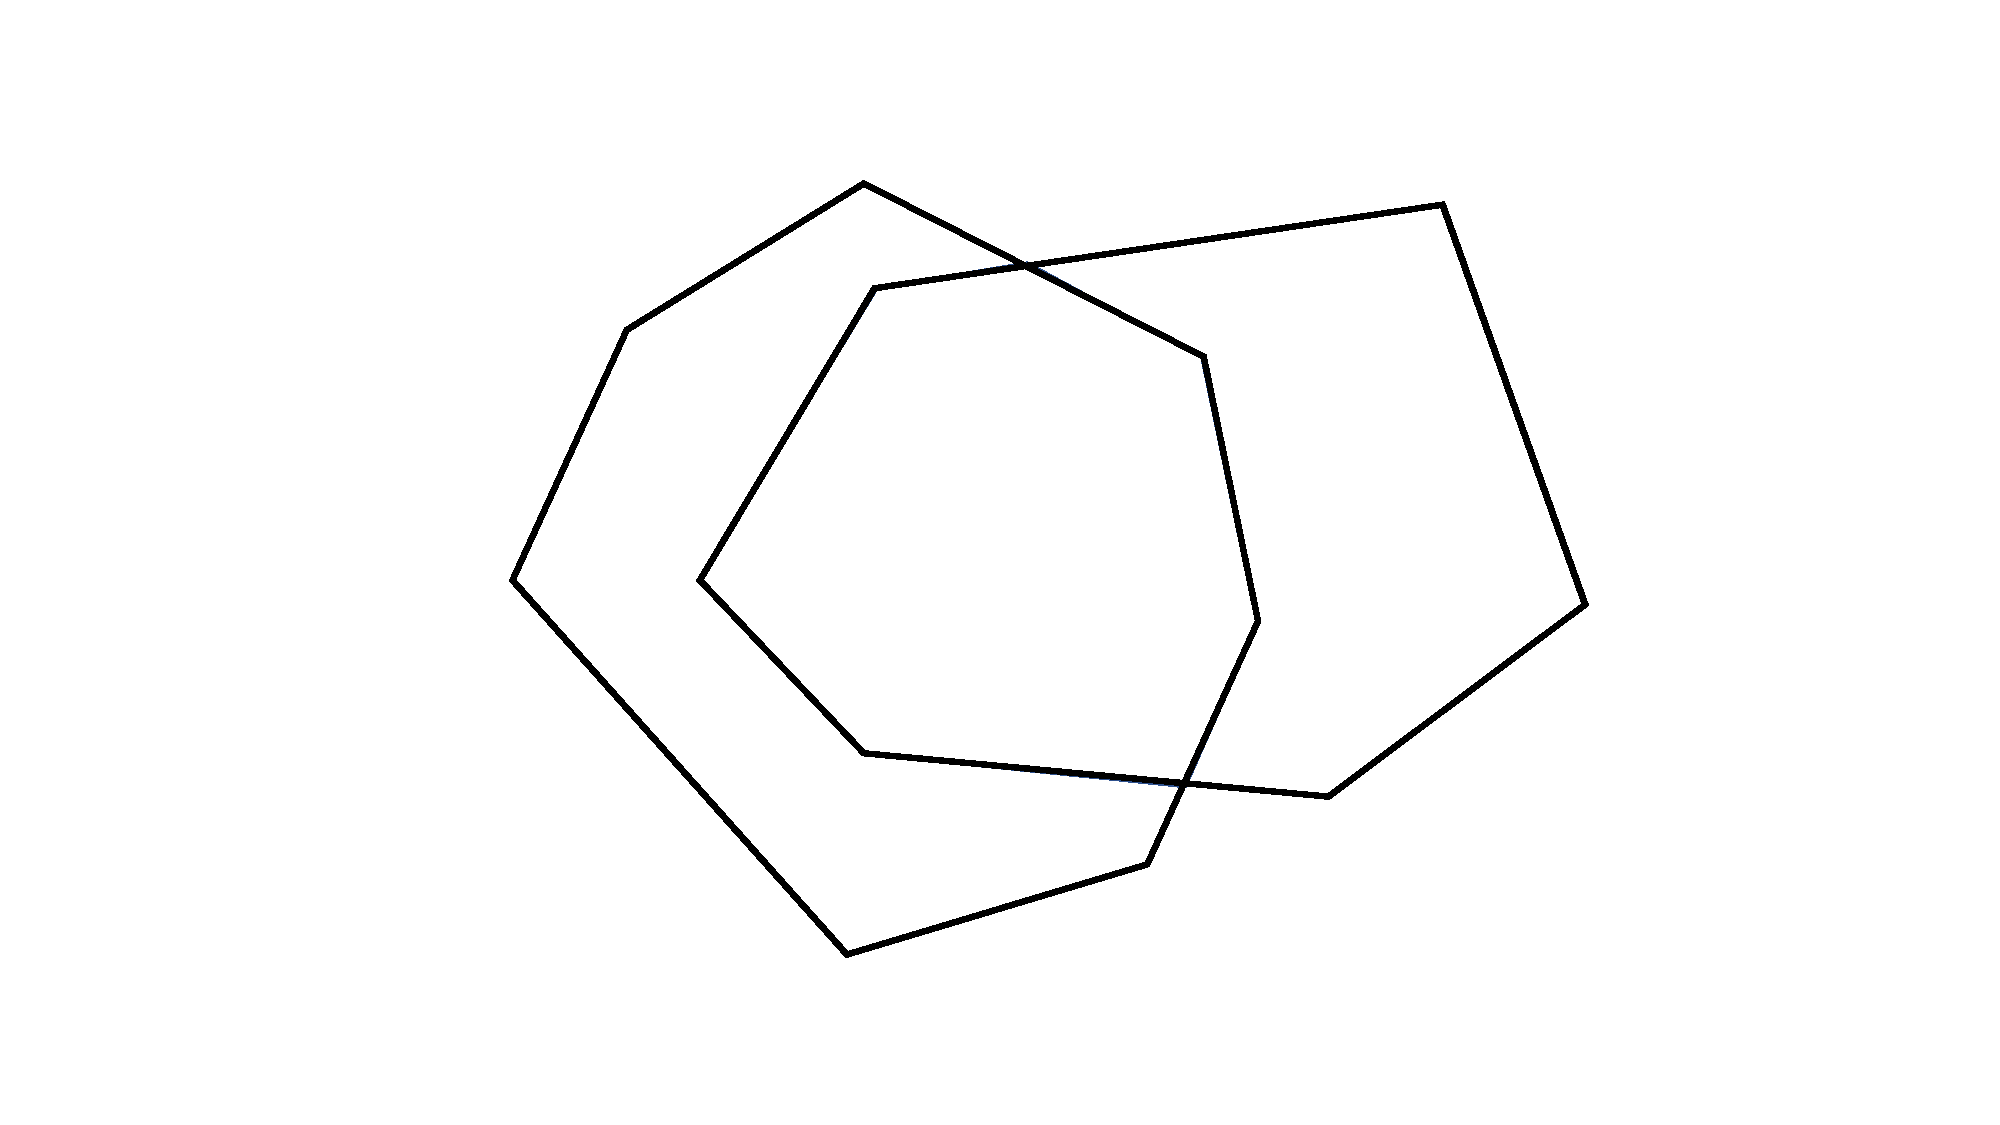
\includegraphics[width=0.3\linewidth]{../images/worksheet2b_no_color.pdf}

\vspace{25pt}
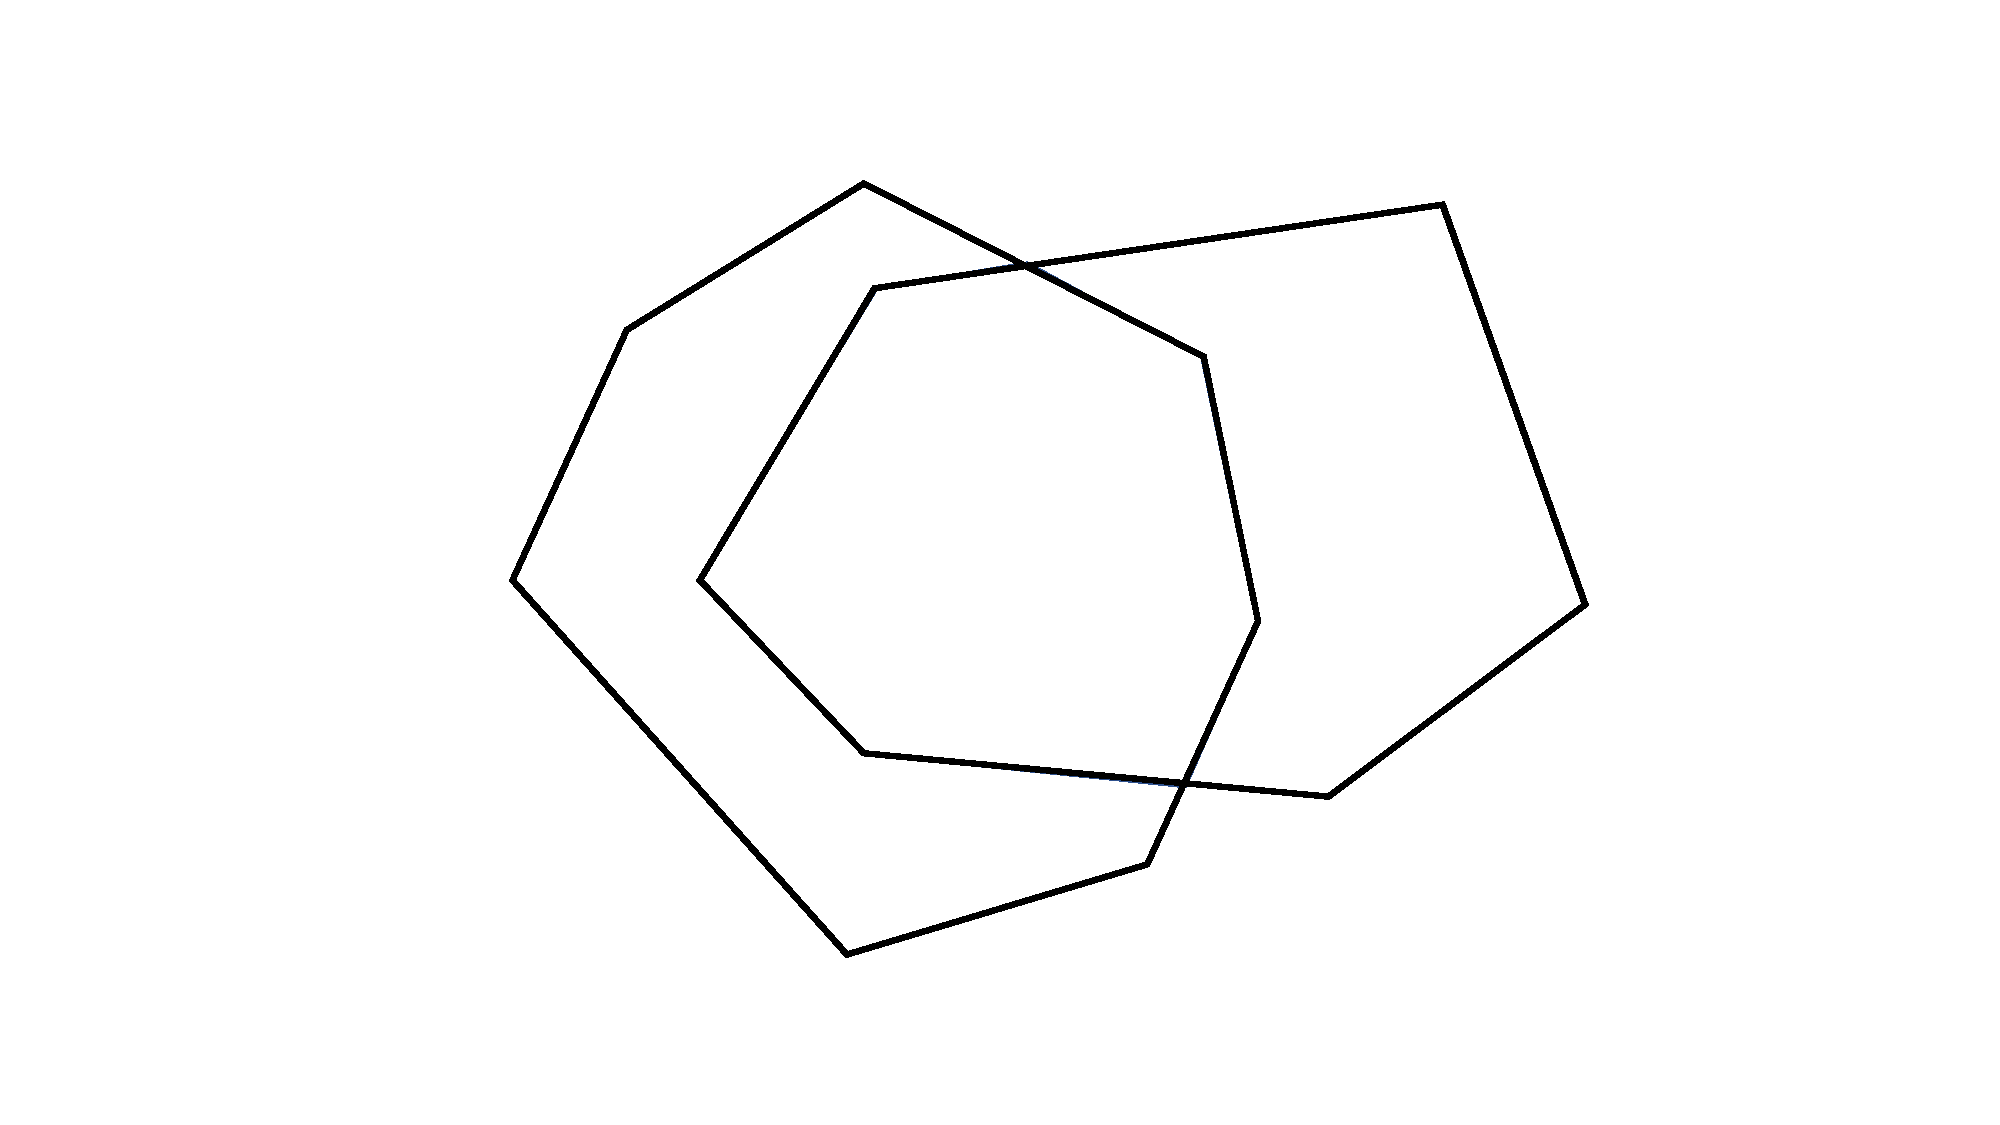
\includegraphics[width=0.3\linewidth]{../images/worksheet2b_no_color.pdf}\hfill
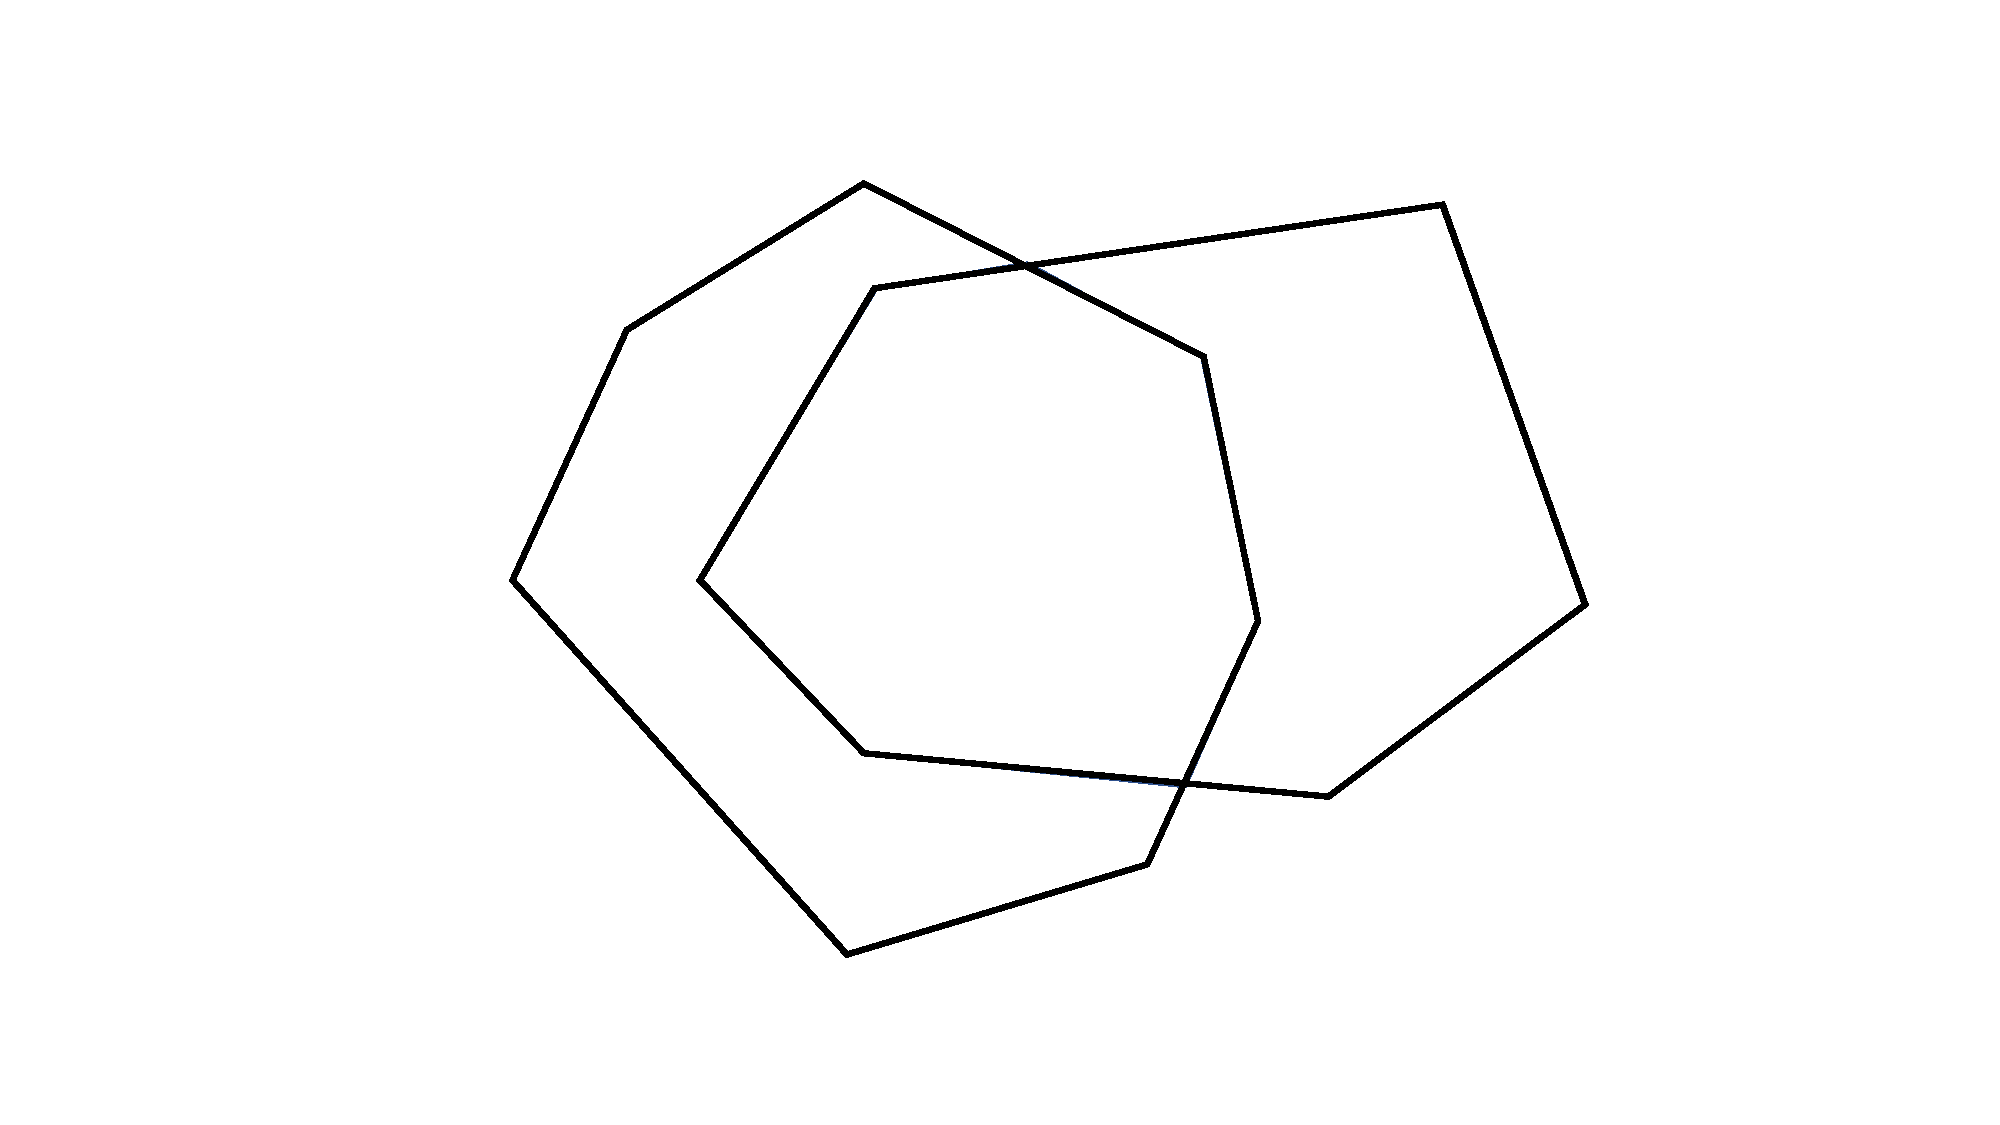
\includegraphics[width=0.3\linewidth]{../images/worksheet2b_no_color.pdf}\hfill
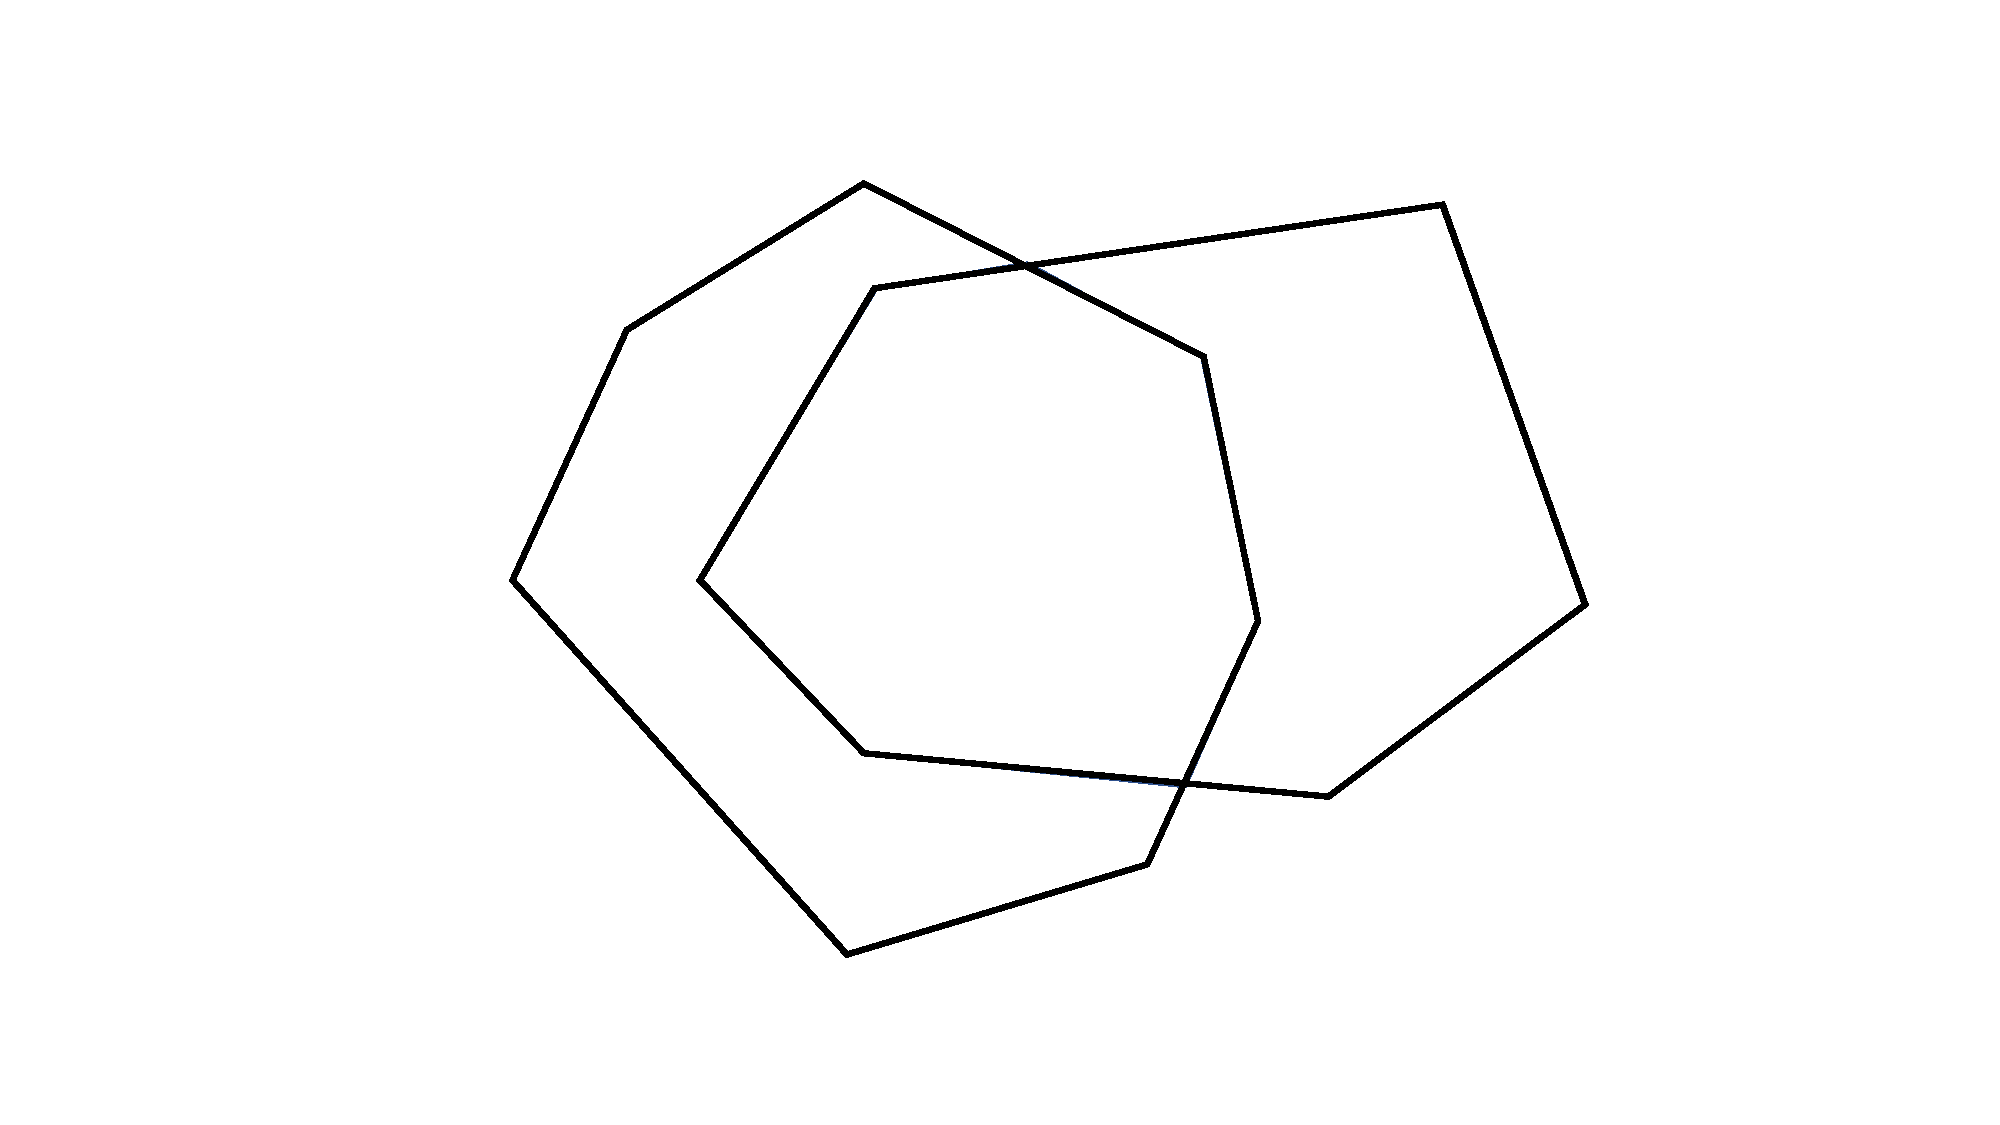
\includegraphics[width=0.3\linewidth]{../images/worksheet2b_no_color.pdf}

\vspace{25pt}
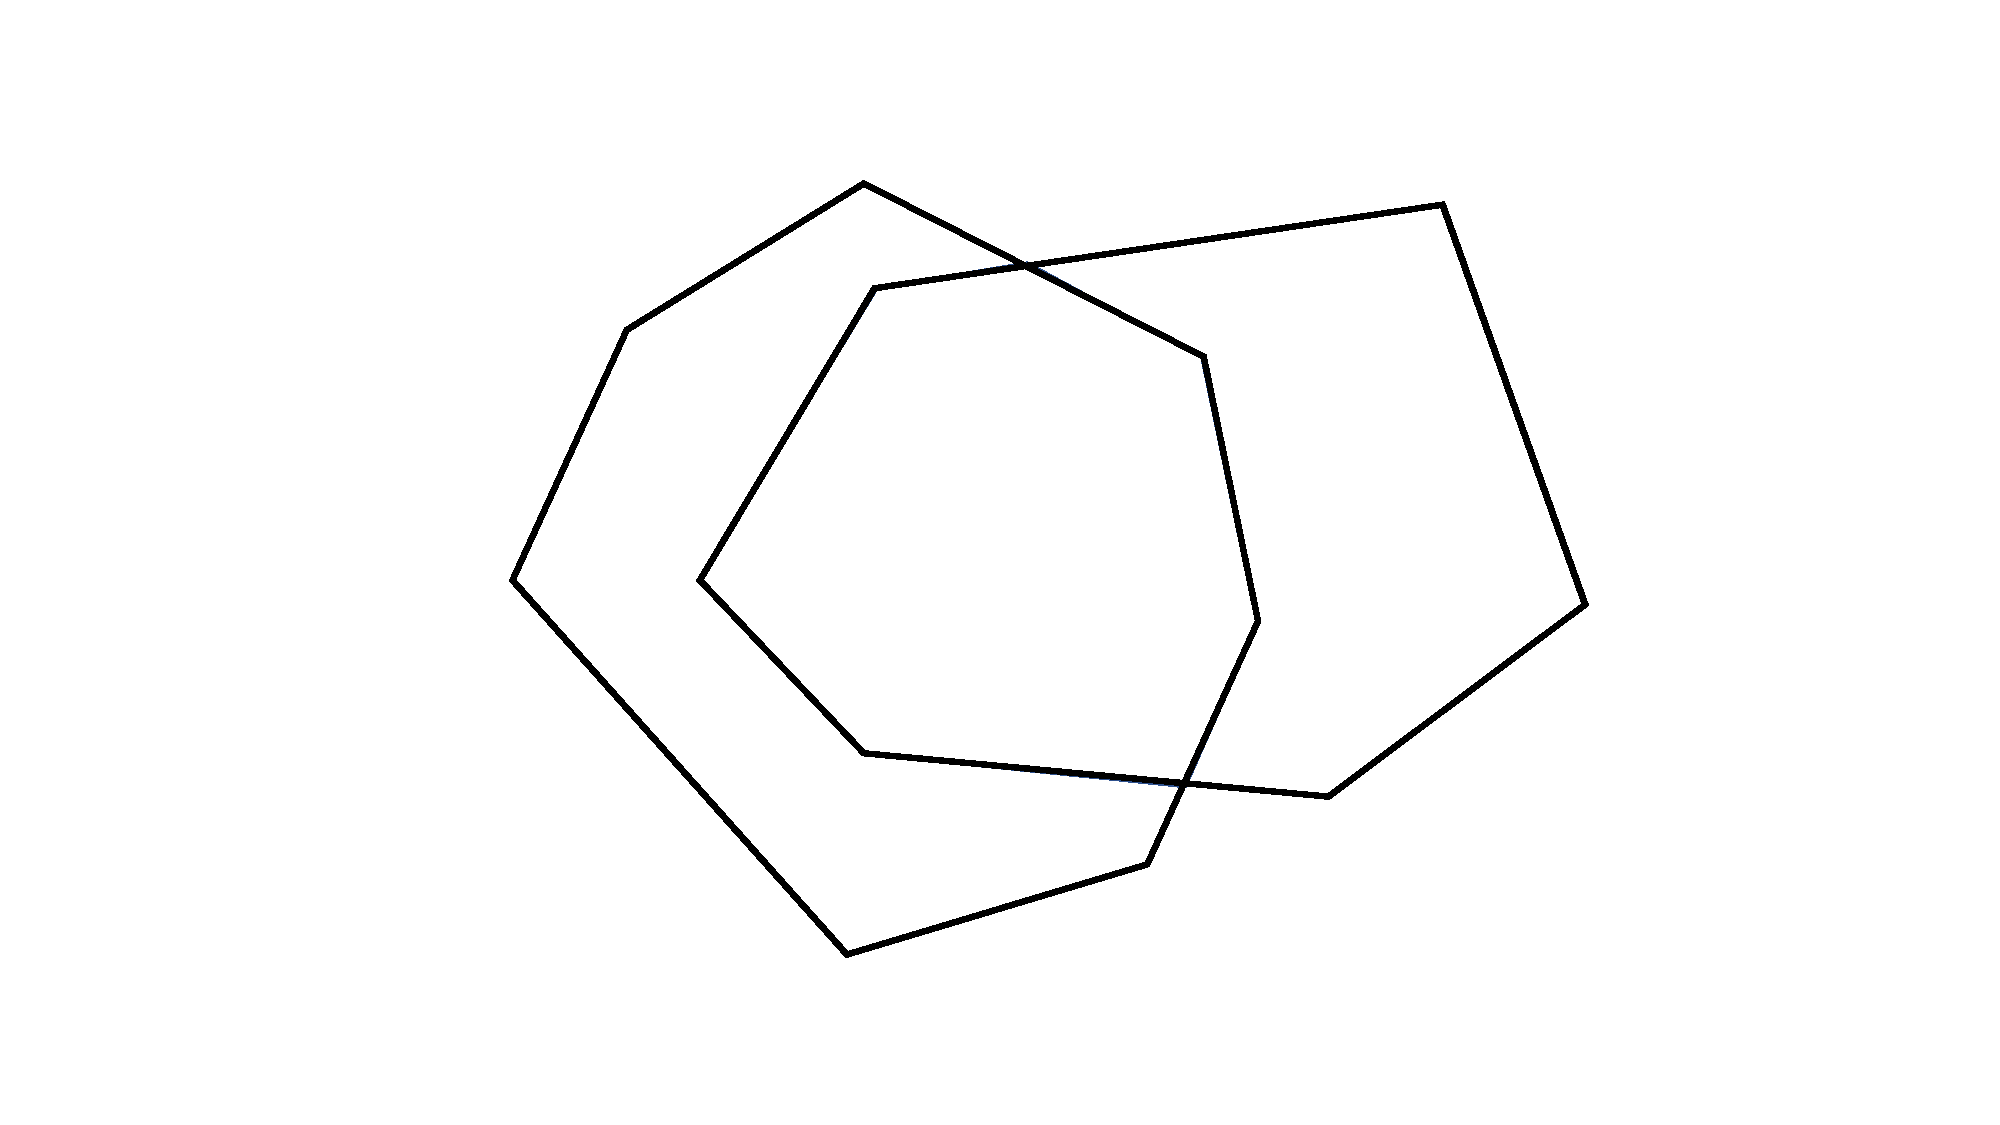
\includegraphics[width=0.3\linewidth]{../images/worksheet2b_no_color.pdf}\hfill
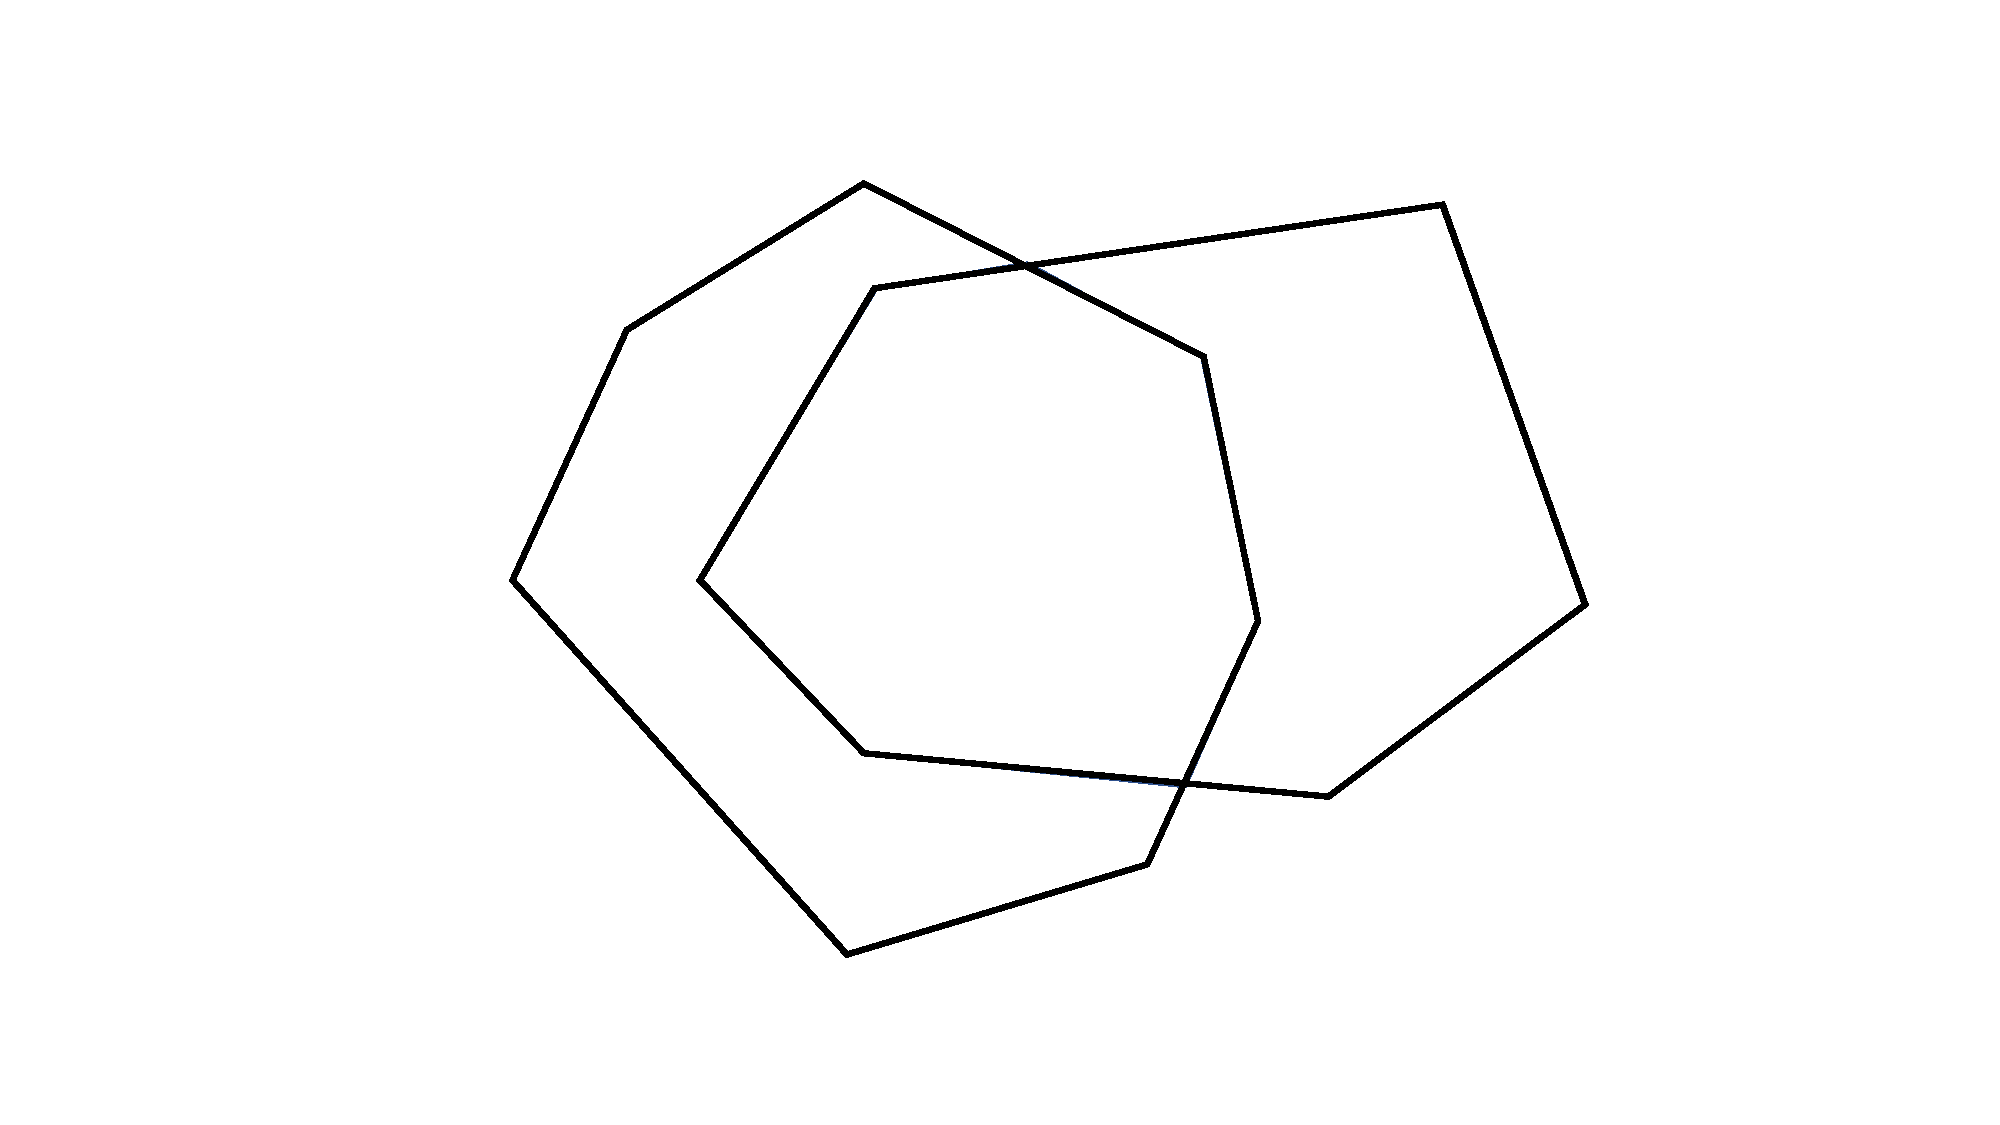
\includegraphics[width=0.3\linewidth]{../images/worksheet2b_no_color.pdf}\hfill
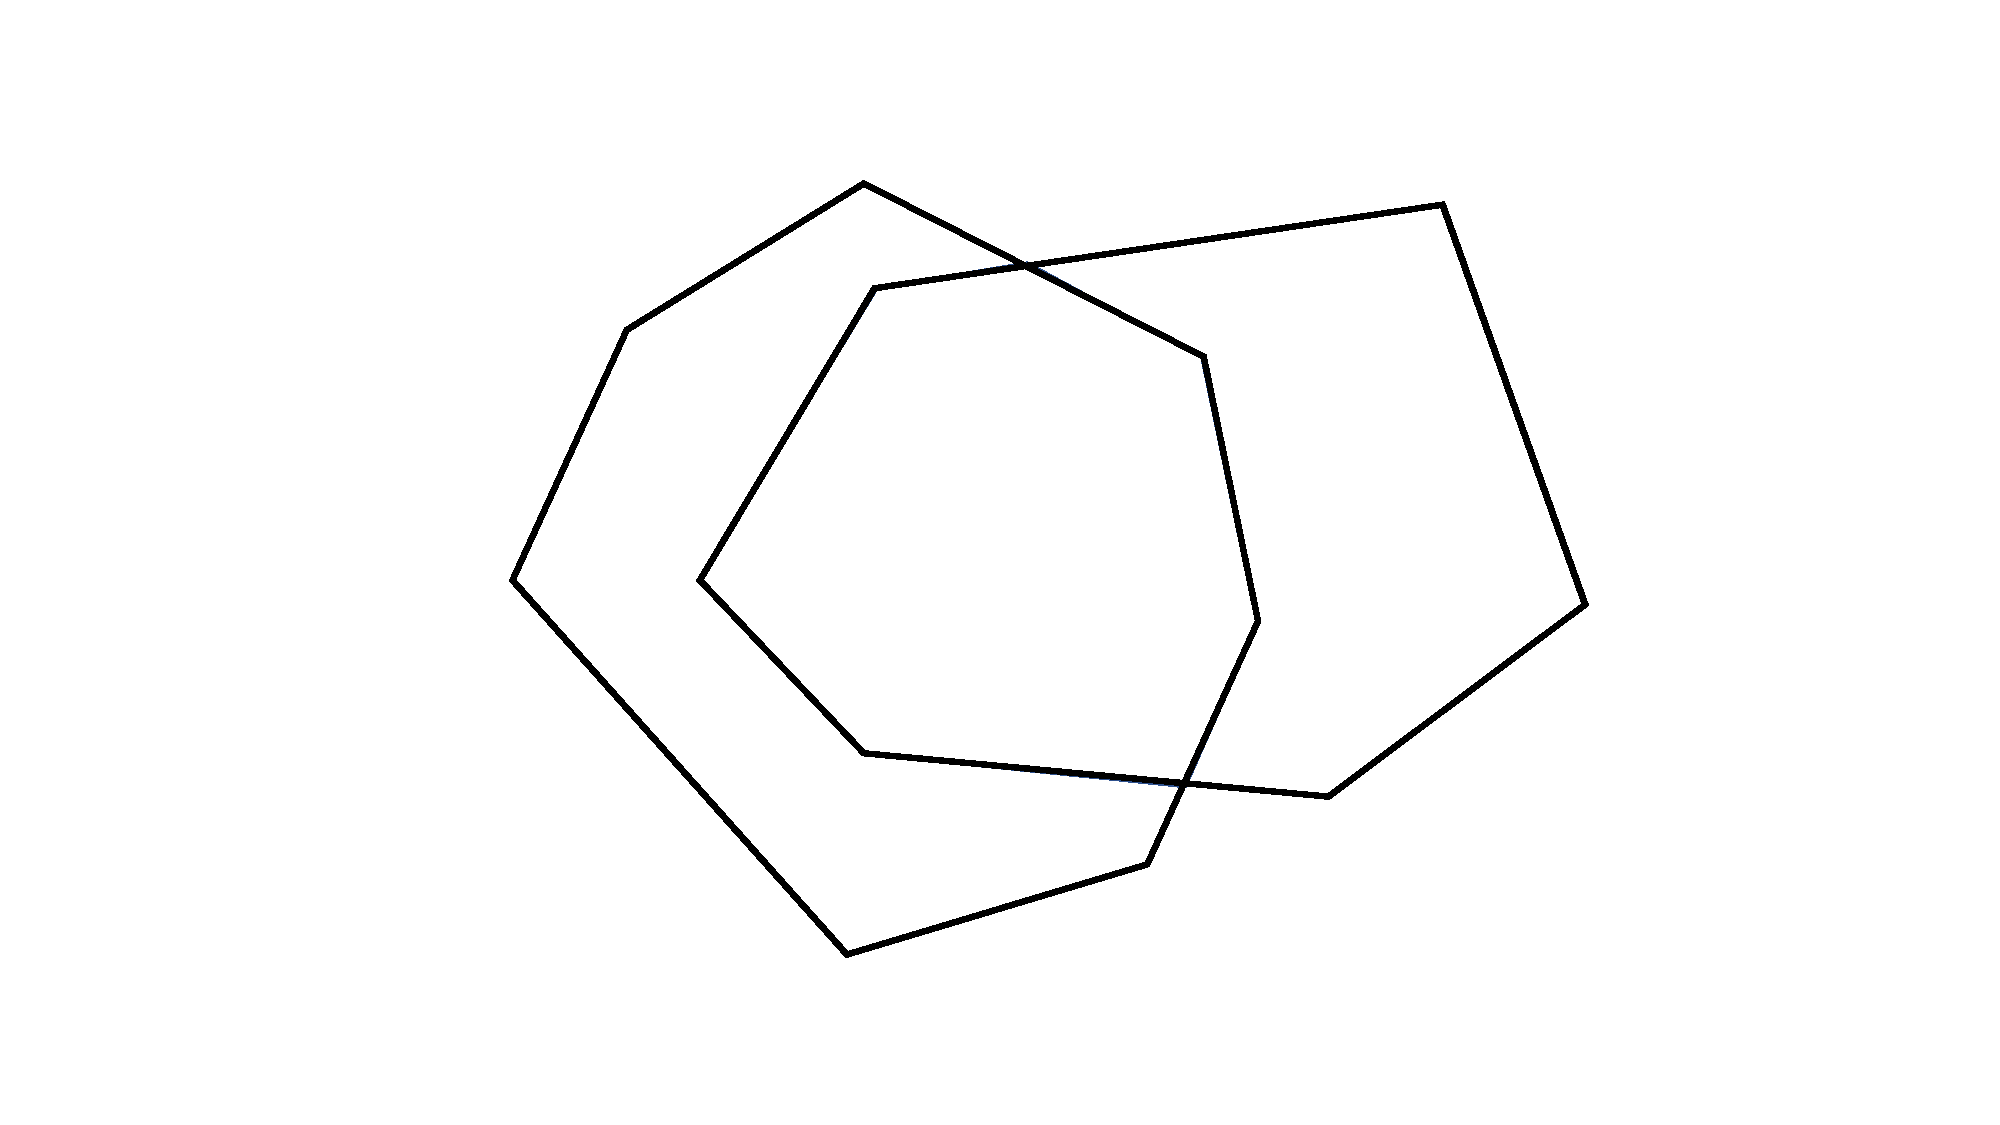
\includegraphics[width=0.3\linewidth]{../images/worksheet2b_no_color.pdf}


\newpage

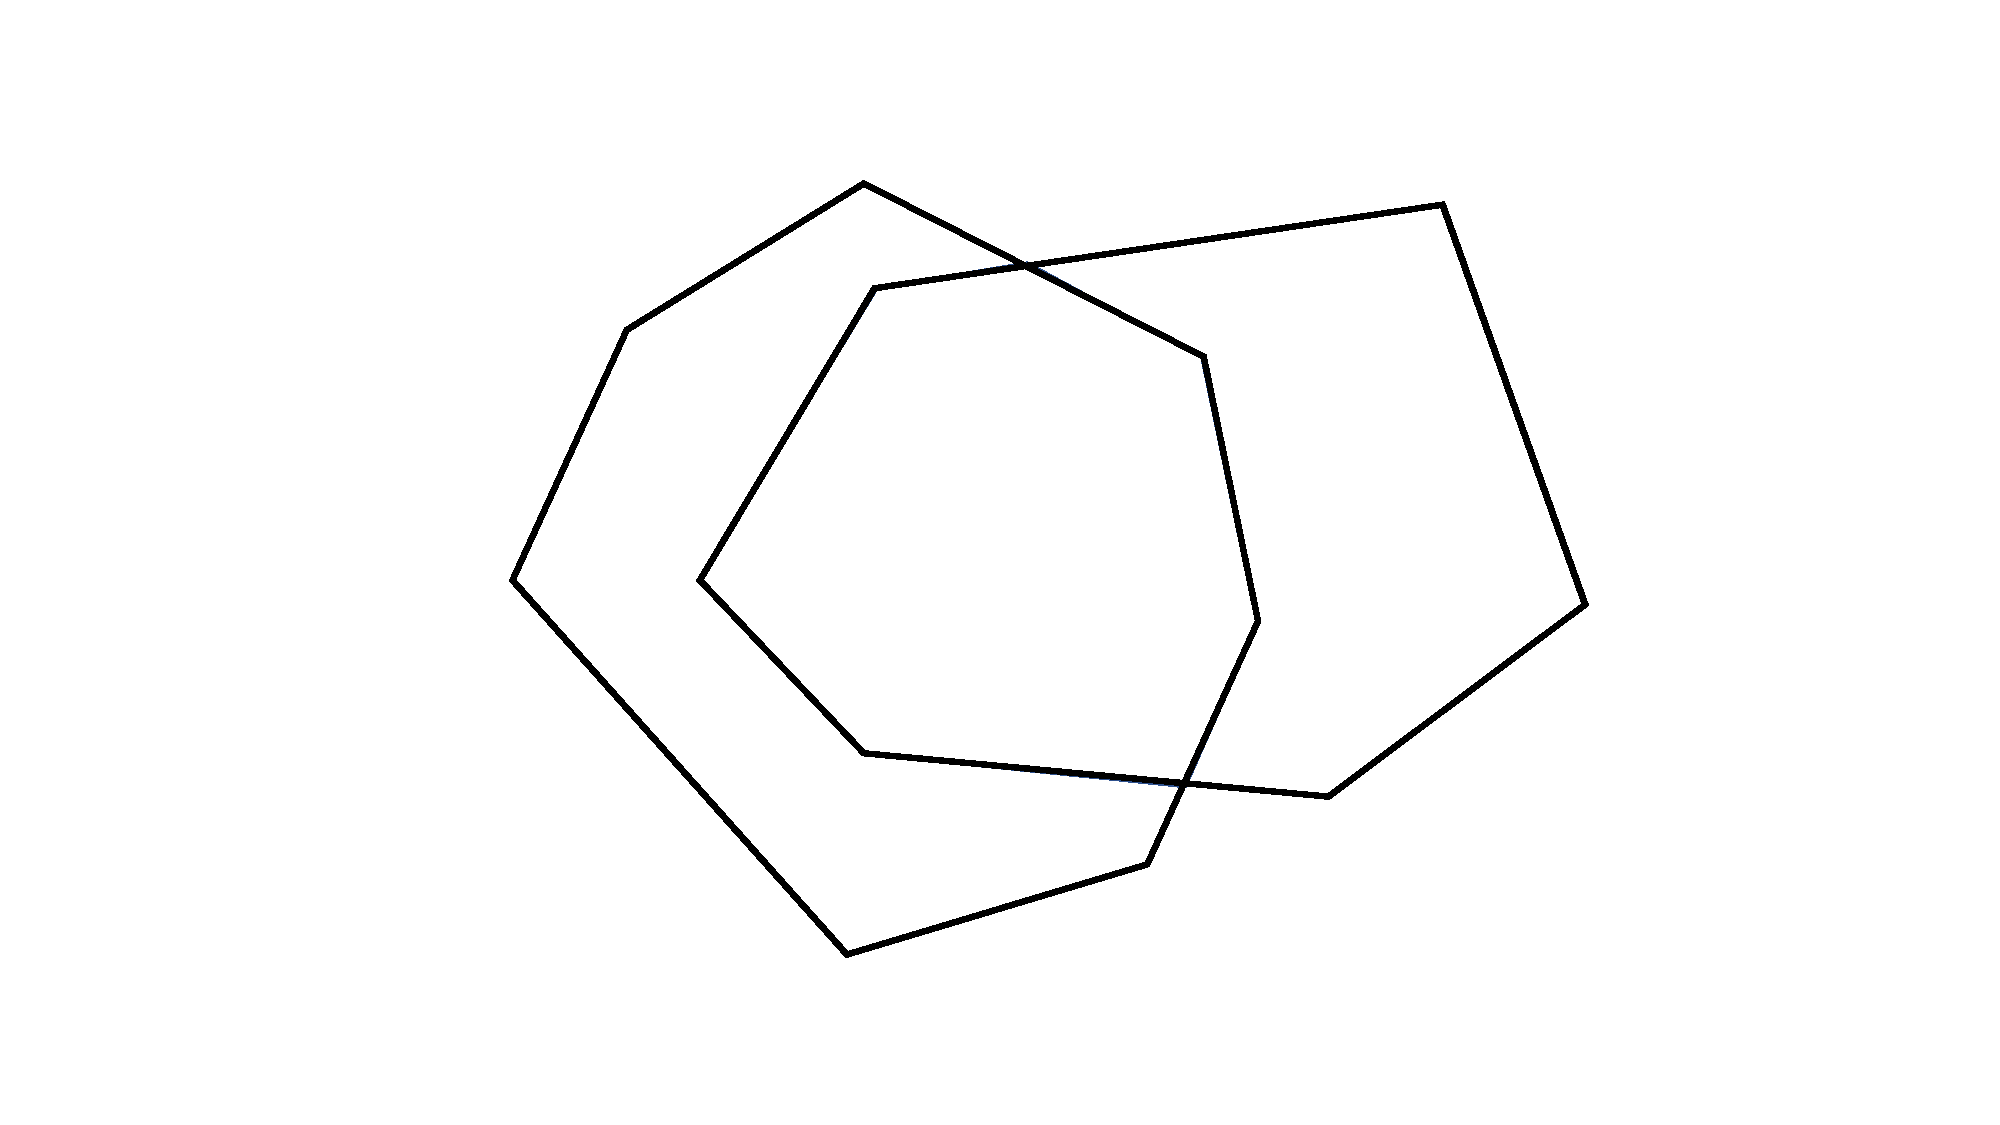
\includegraphics[width=0.3\linewidth]{../images/worksheet2b_no_color.pdf}\hfill
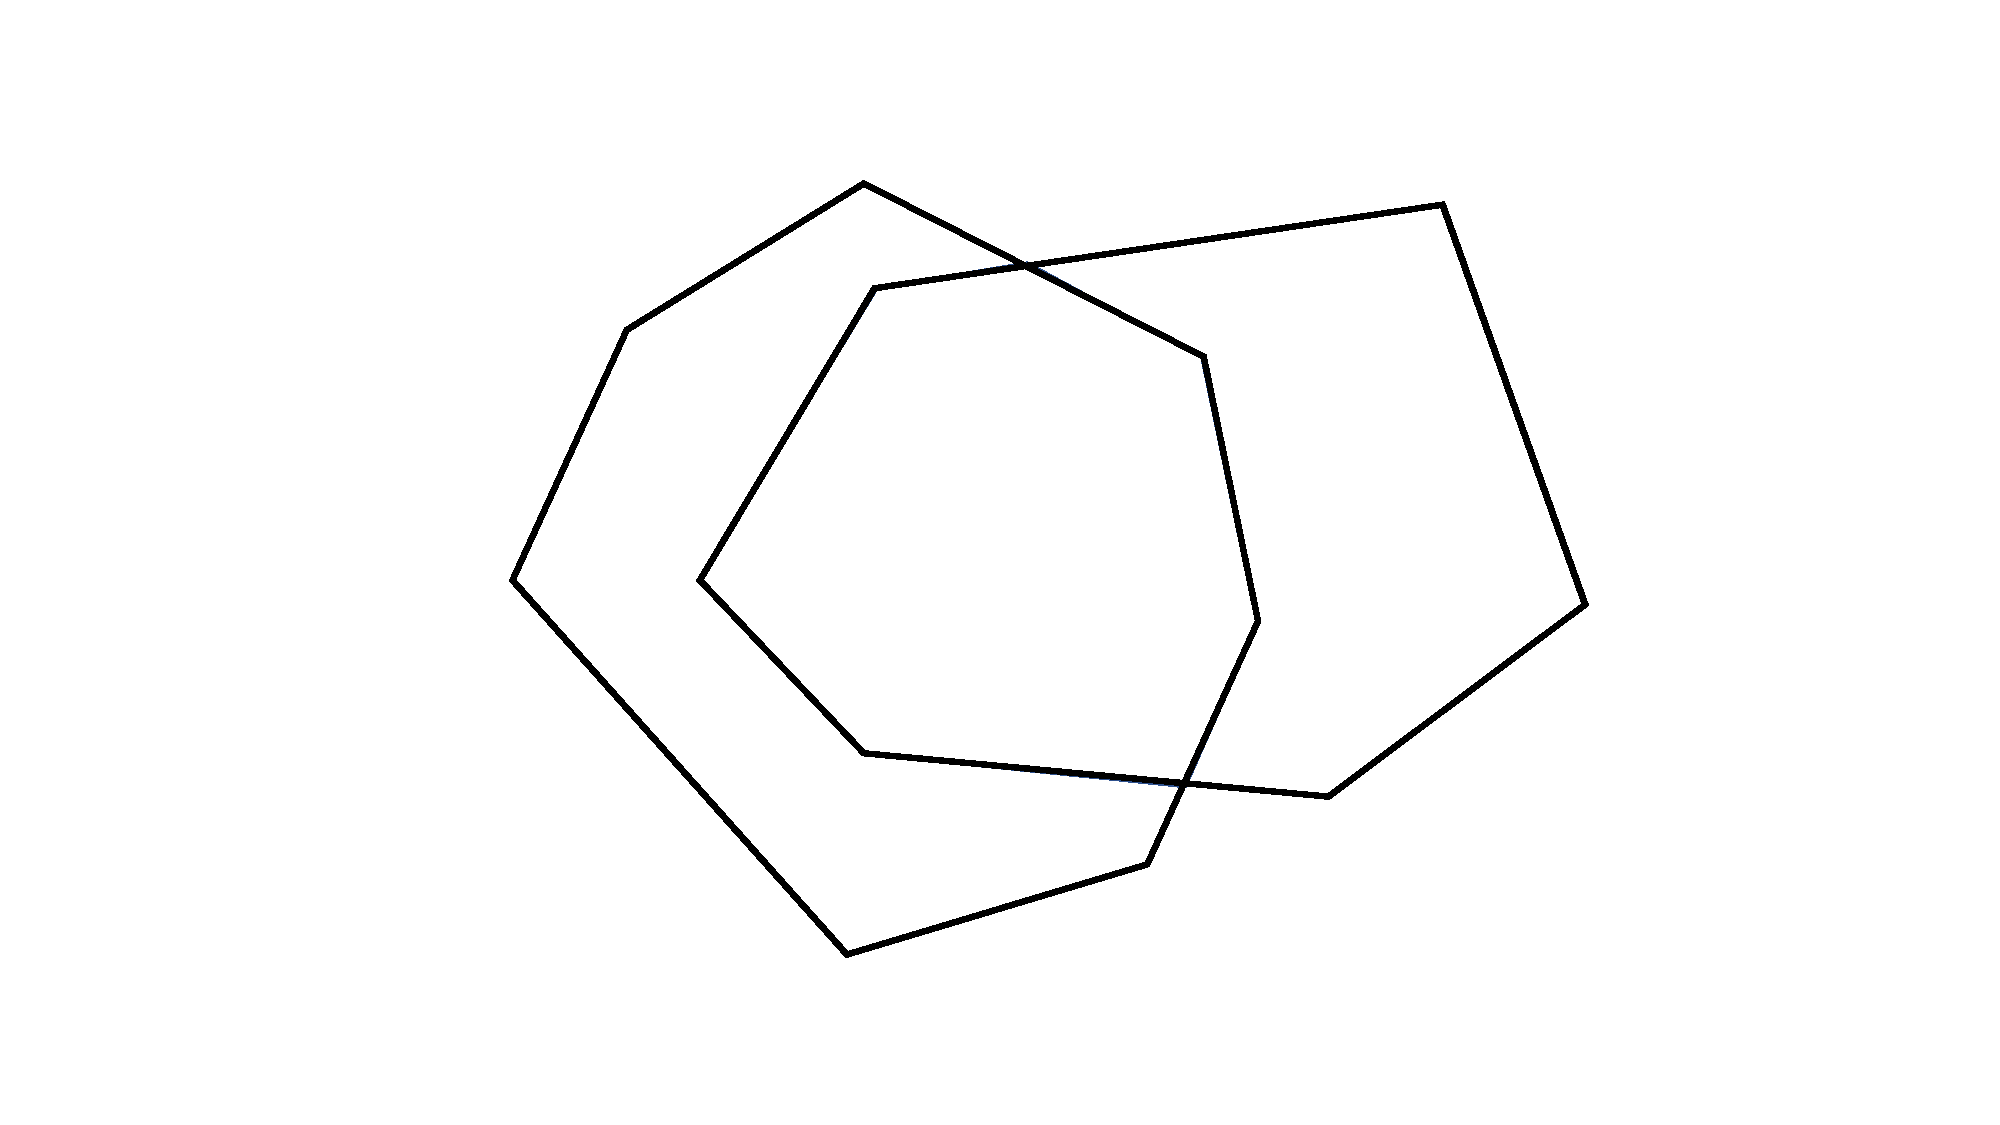
\includegraphics[width=0.3\linewidth]{../images/worksheet2b_no_color.pdf}\hfill
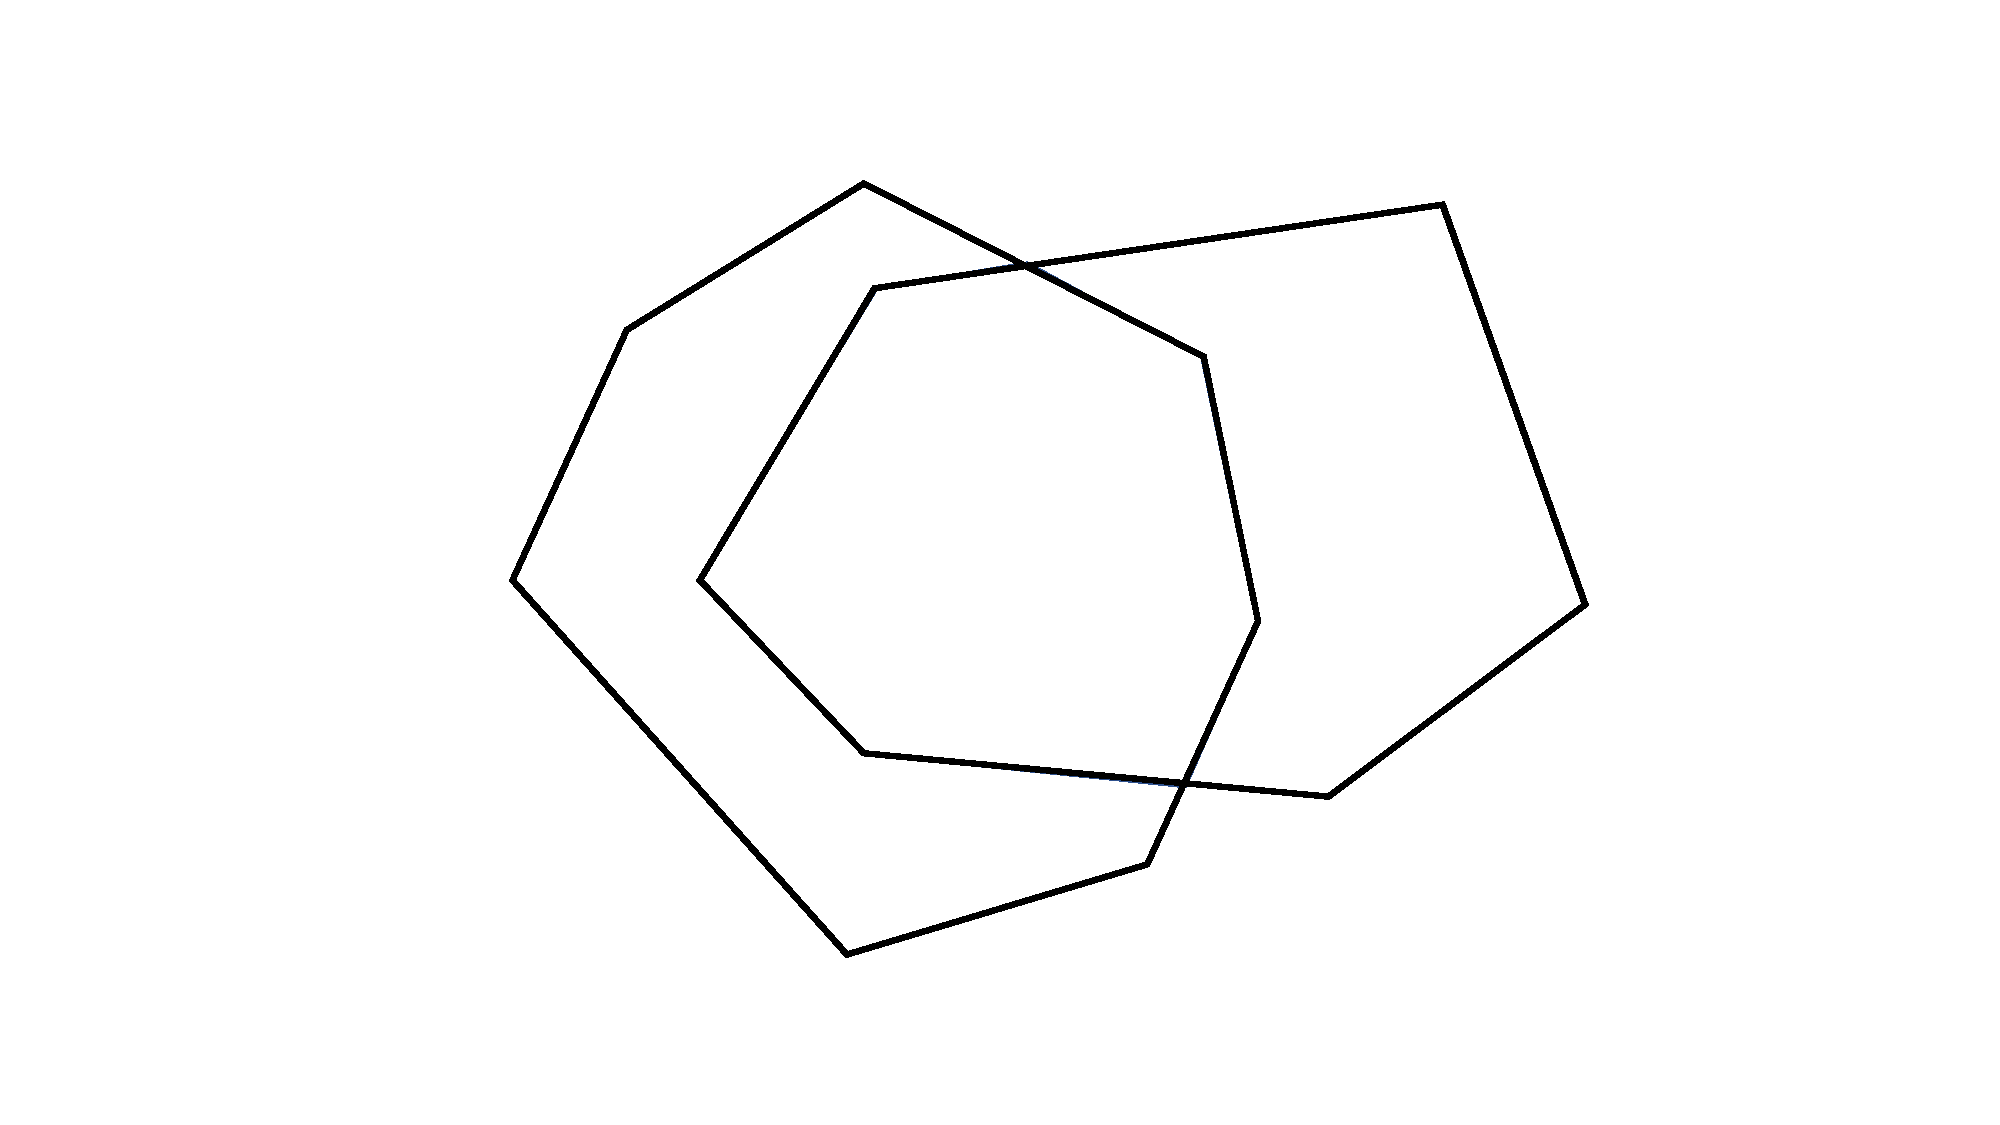
\includegraphics[width=0.3\linewidth]{../images/worksheet2b_no_color.pdf}

\vspace{25pt}
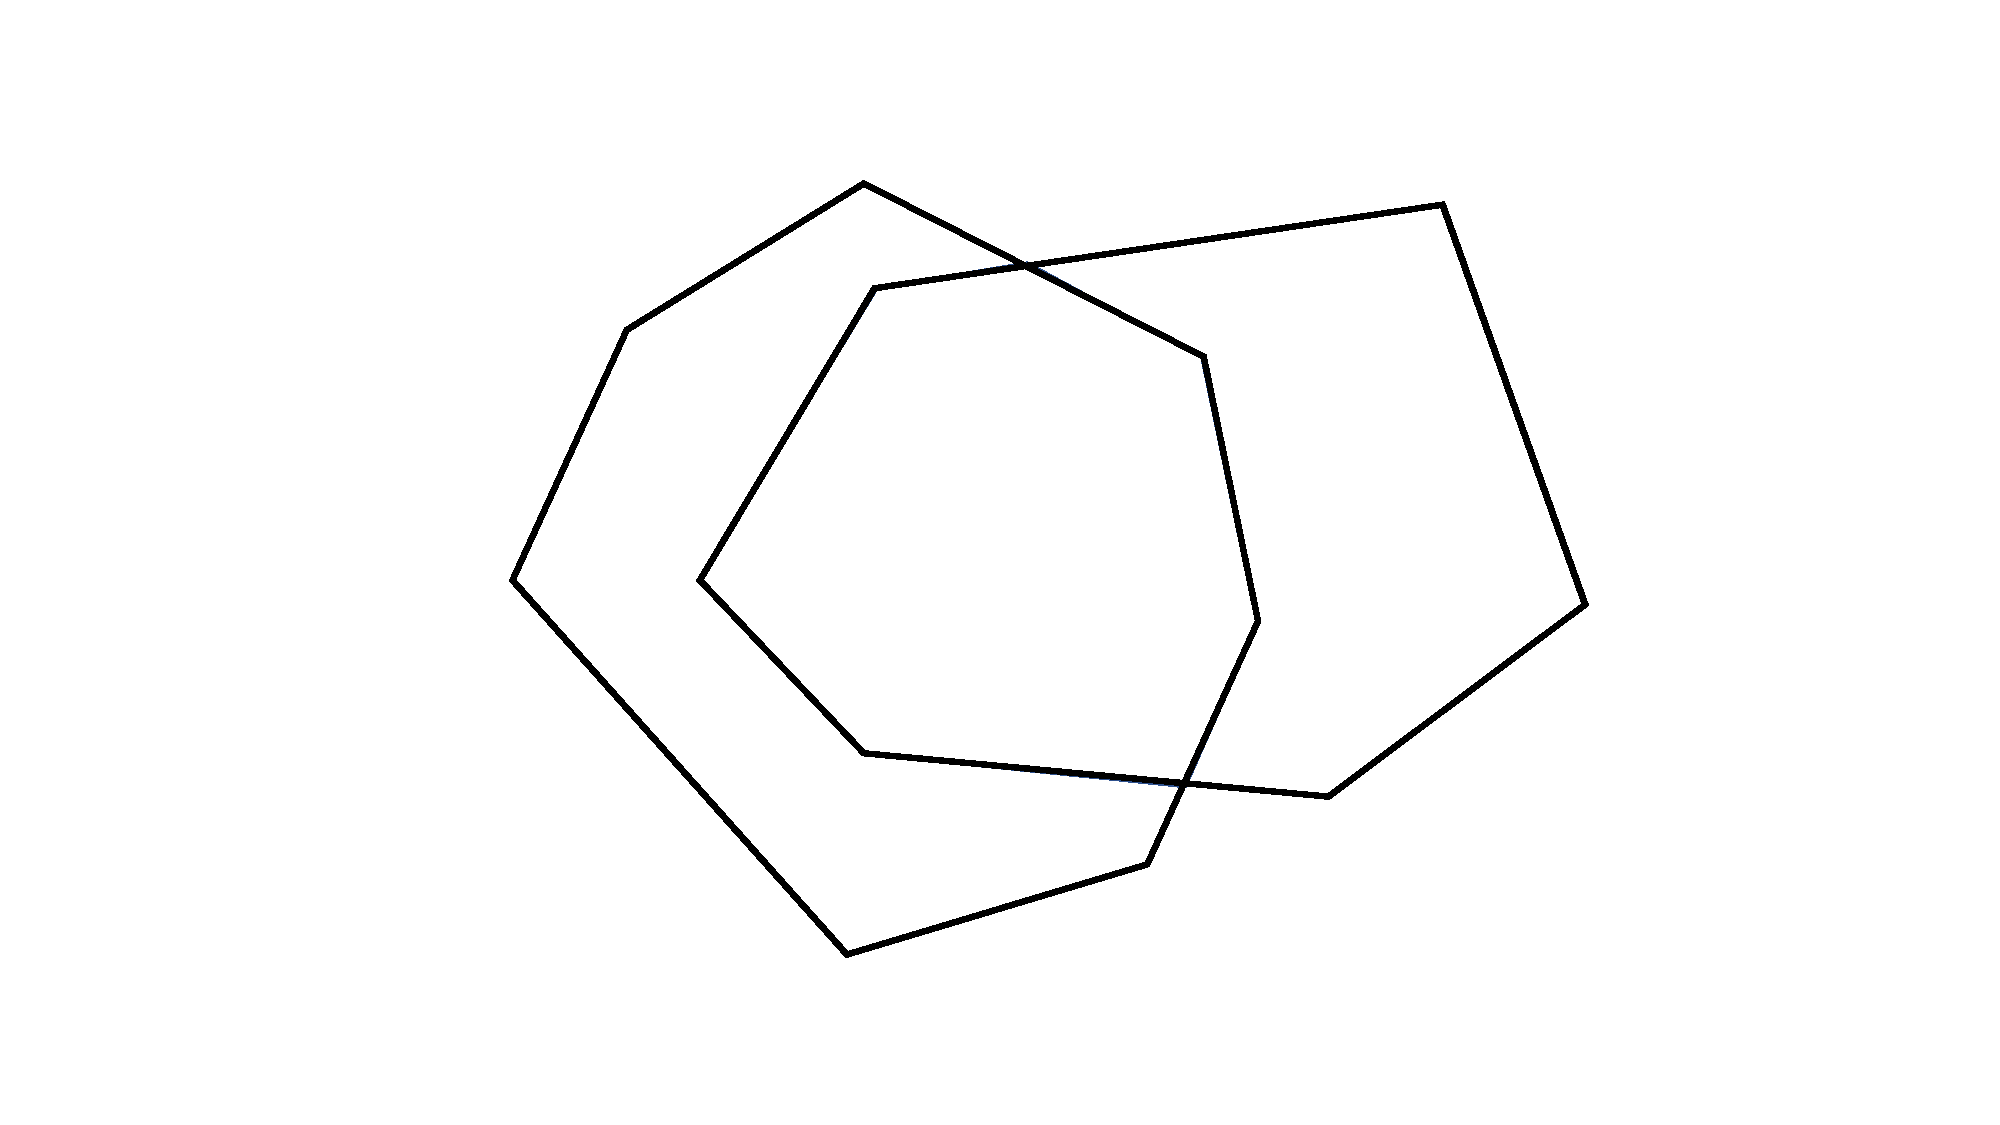
\includegraphics[width=0.3\linewidth]{../images/worksheet2b_no_color.pdf}\hfill
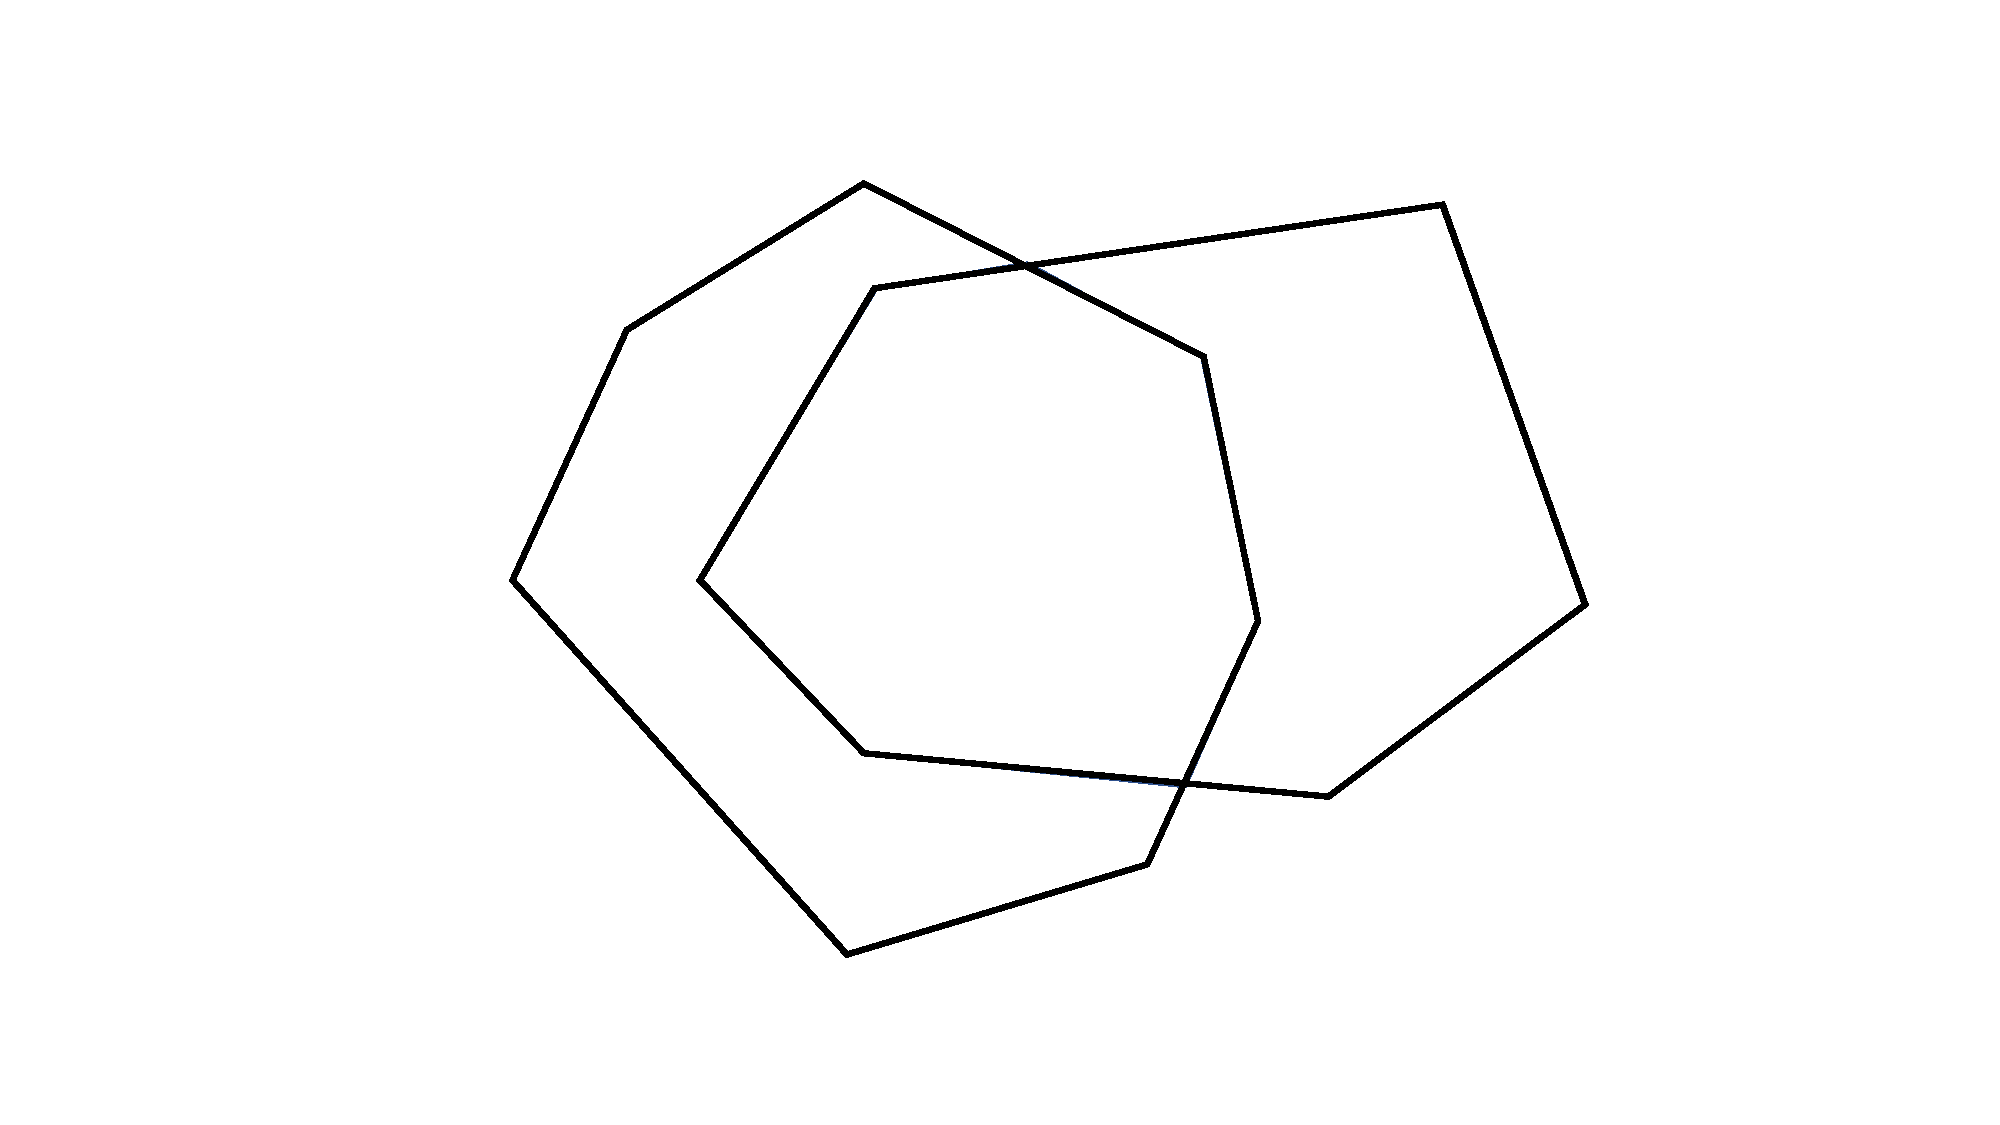
\includegraphics[width=0.3\linewidth]{../images/worksheet2b_no_color.pdf}\hfill
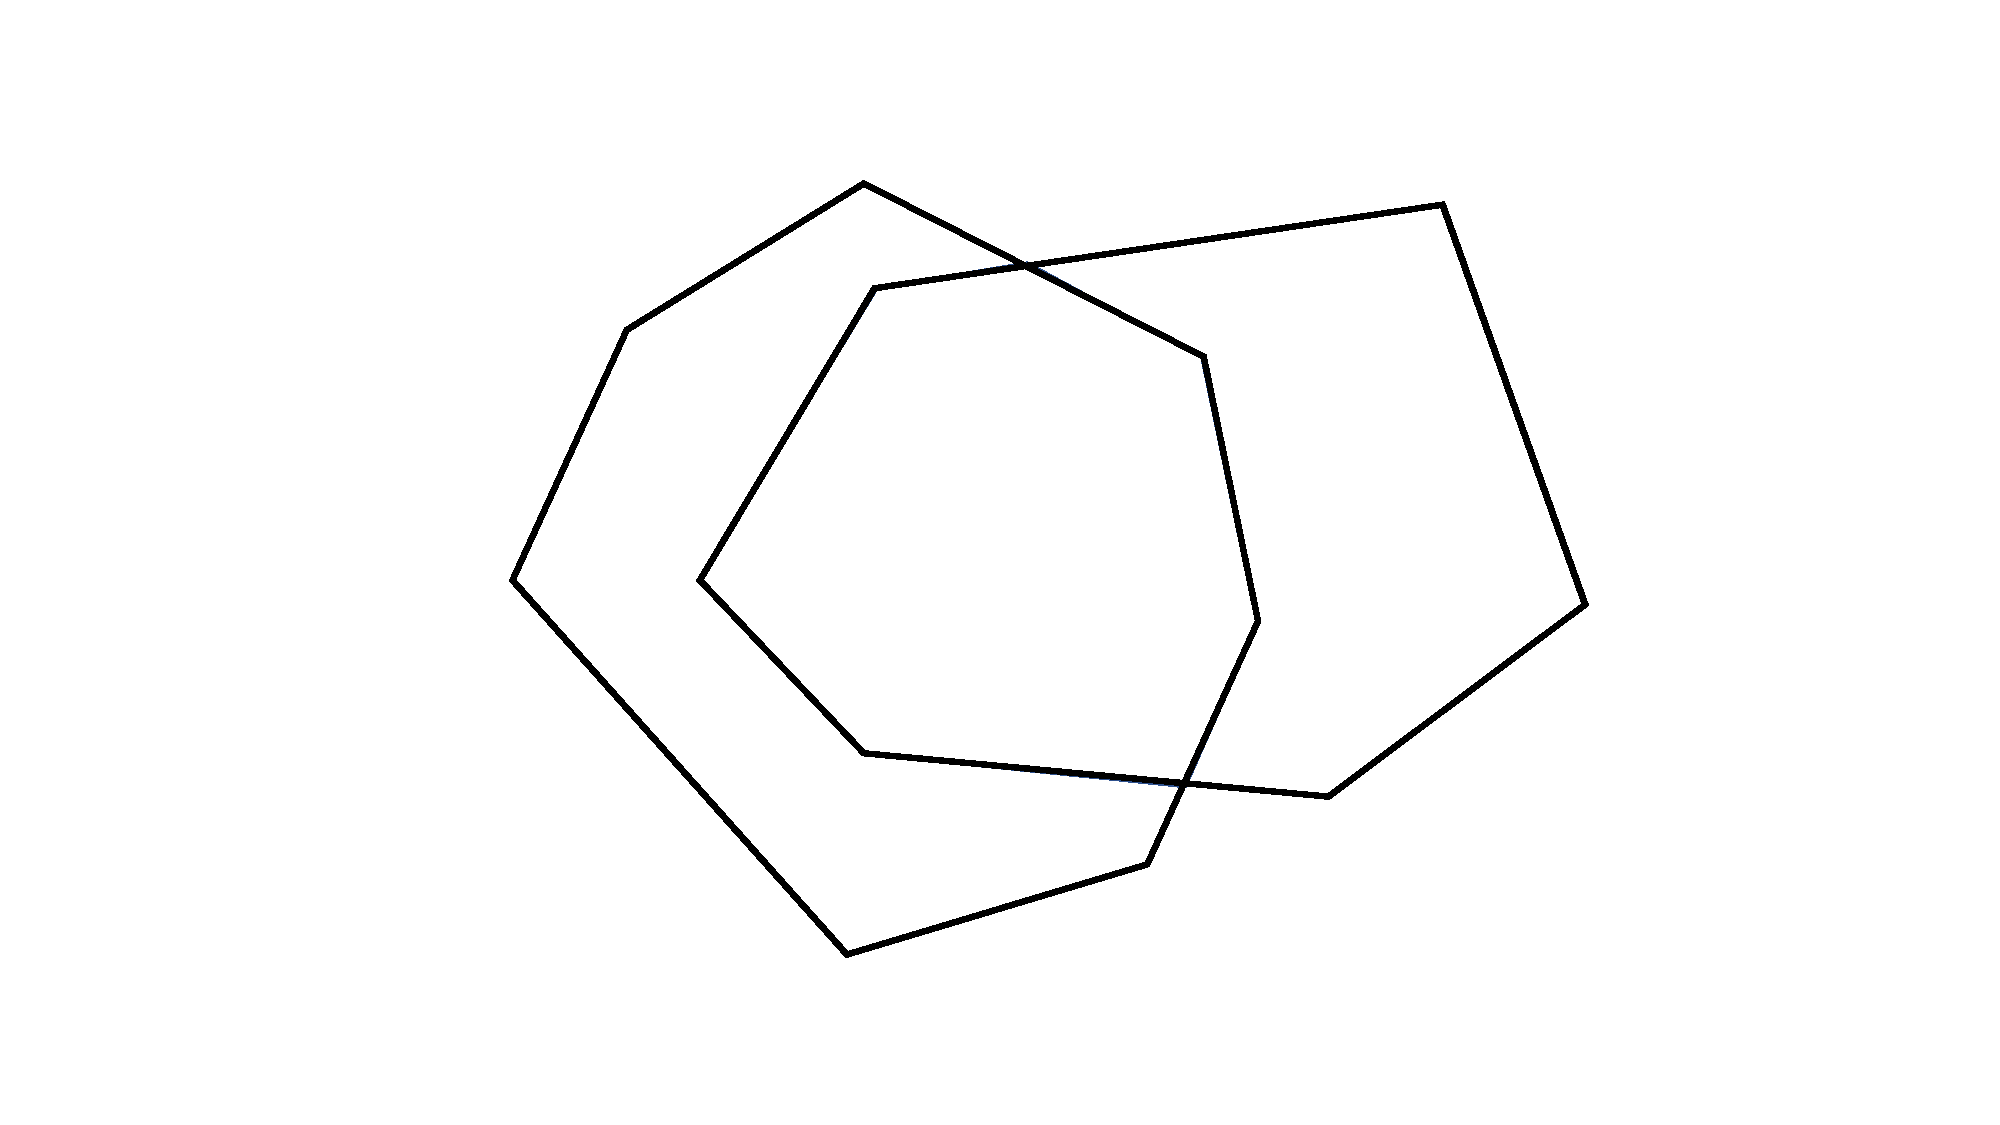
\includegraphics[width=0.3\linewidth]{../images/worksheet2b_no_color.pdf}

\vspace{25pt}
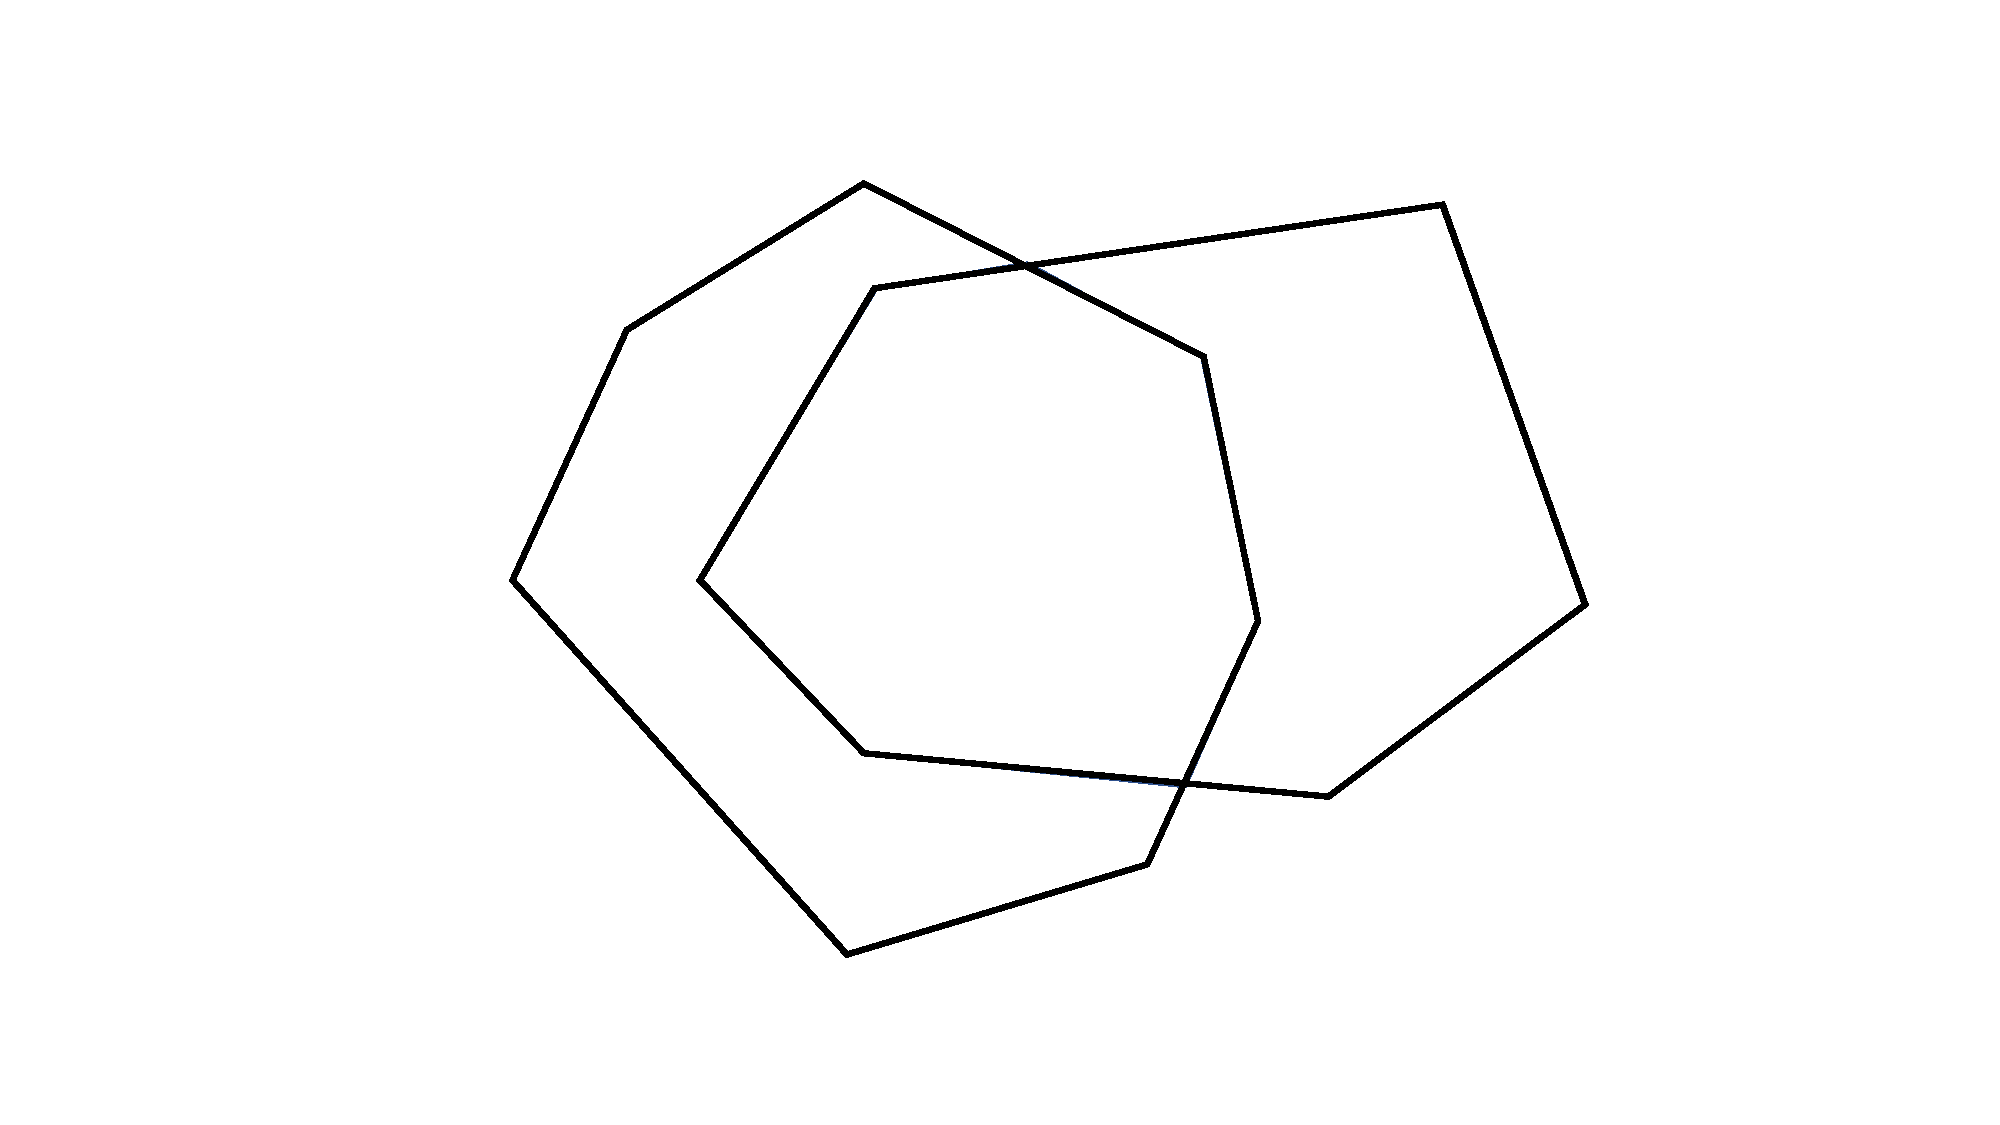
\includegraphics[width=0.3\linewidth]{../images/worksheet2b_no_color.pdf}\hfill
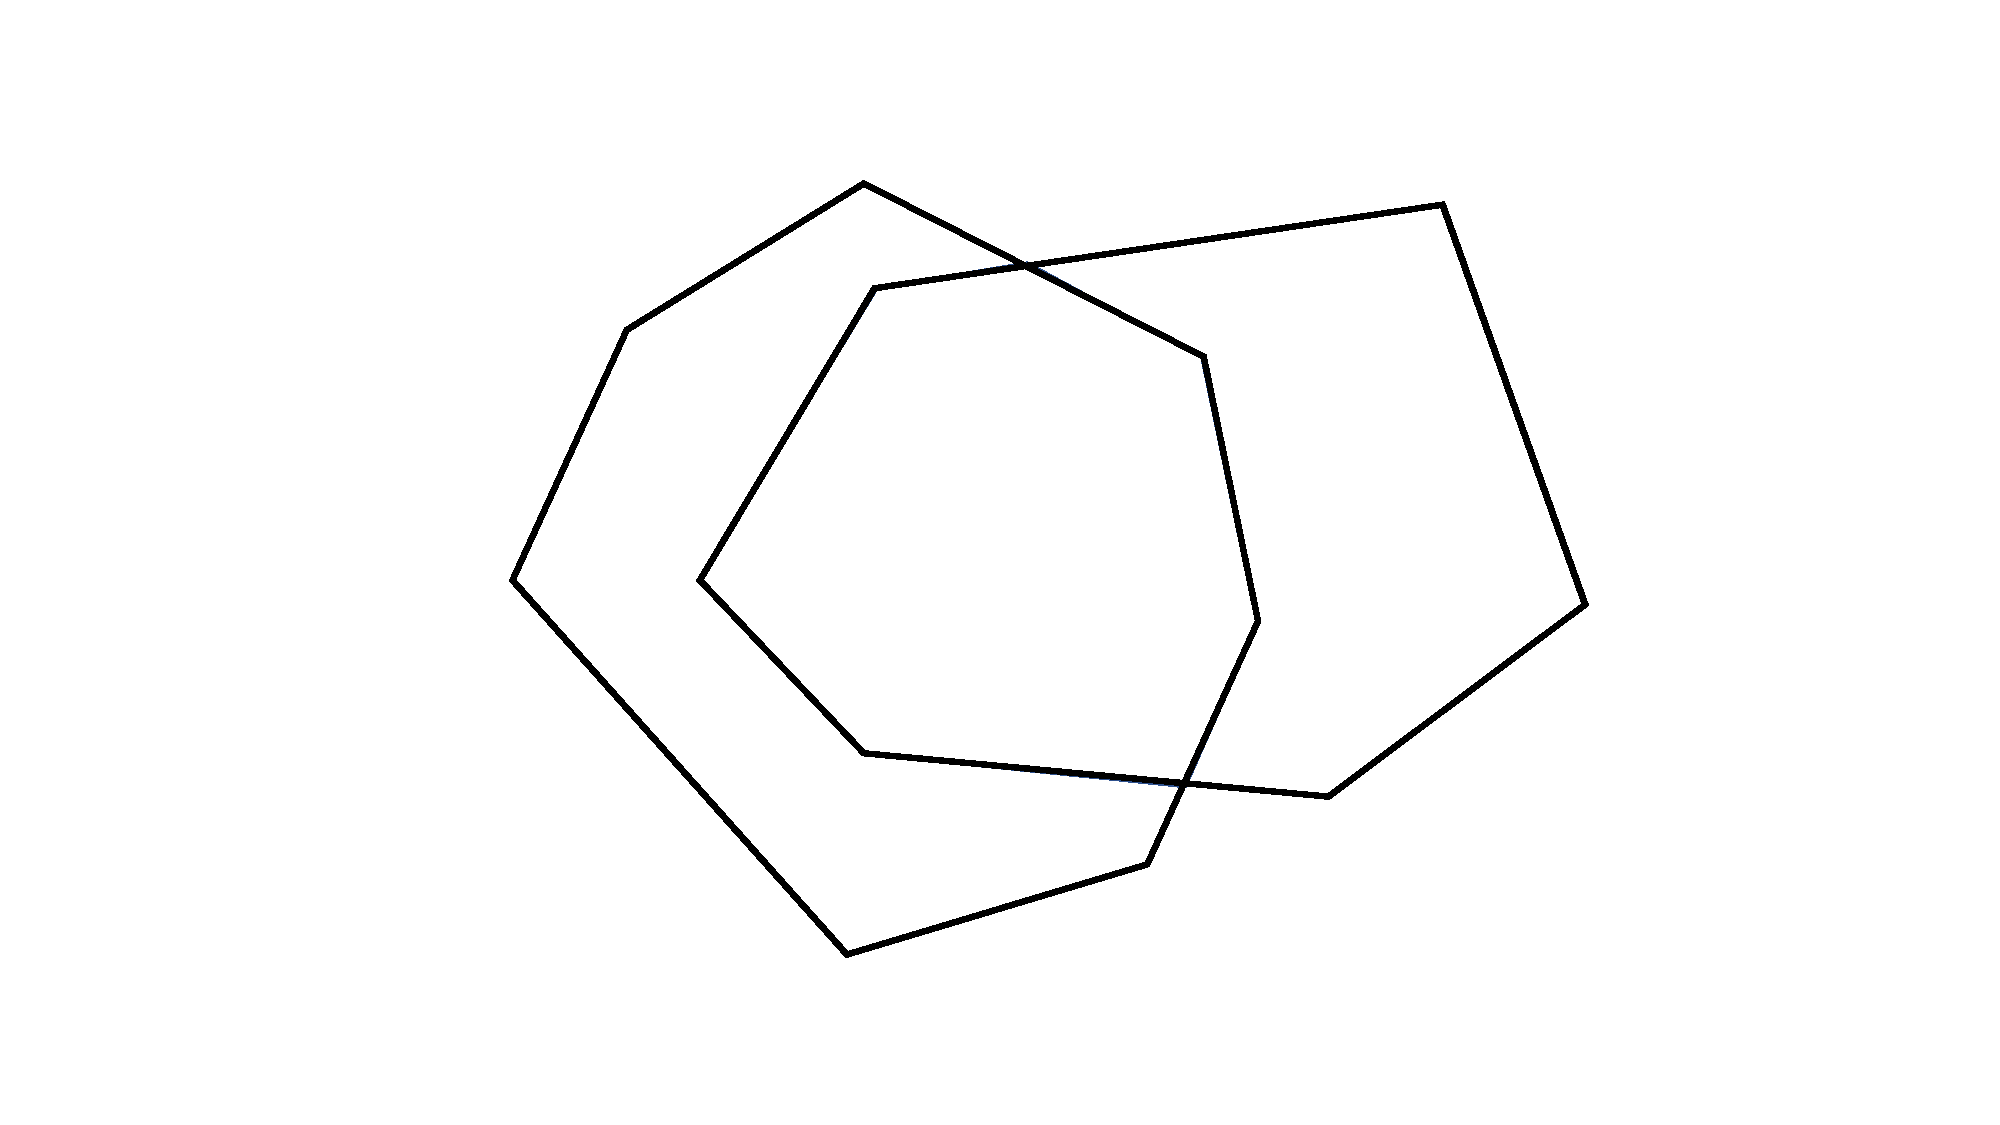
\includegraphics[width=0.3\linewidth]{../images/worksheet2b_no_color.pdf}\hfill
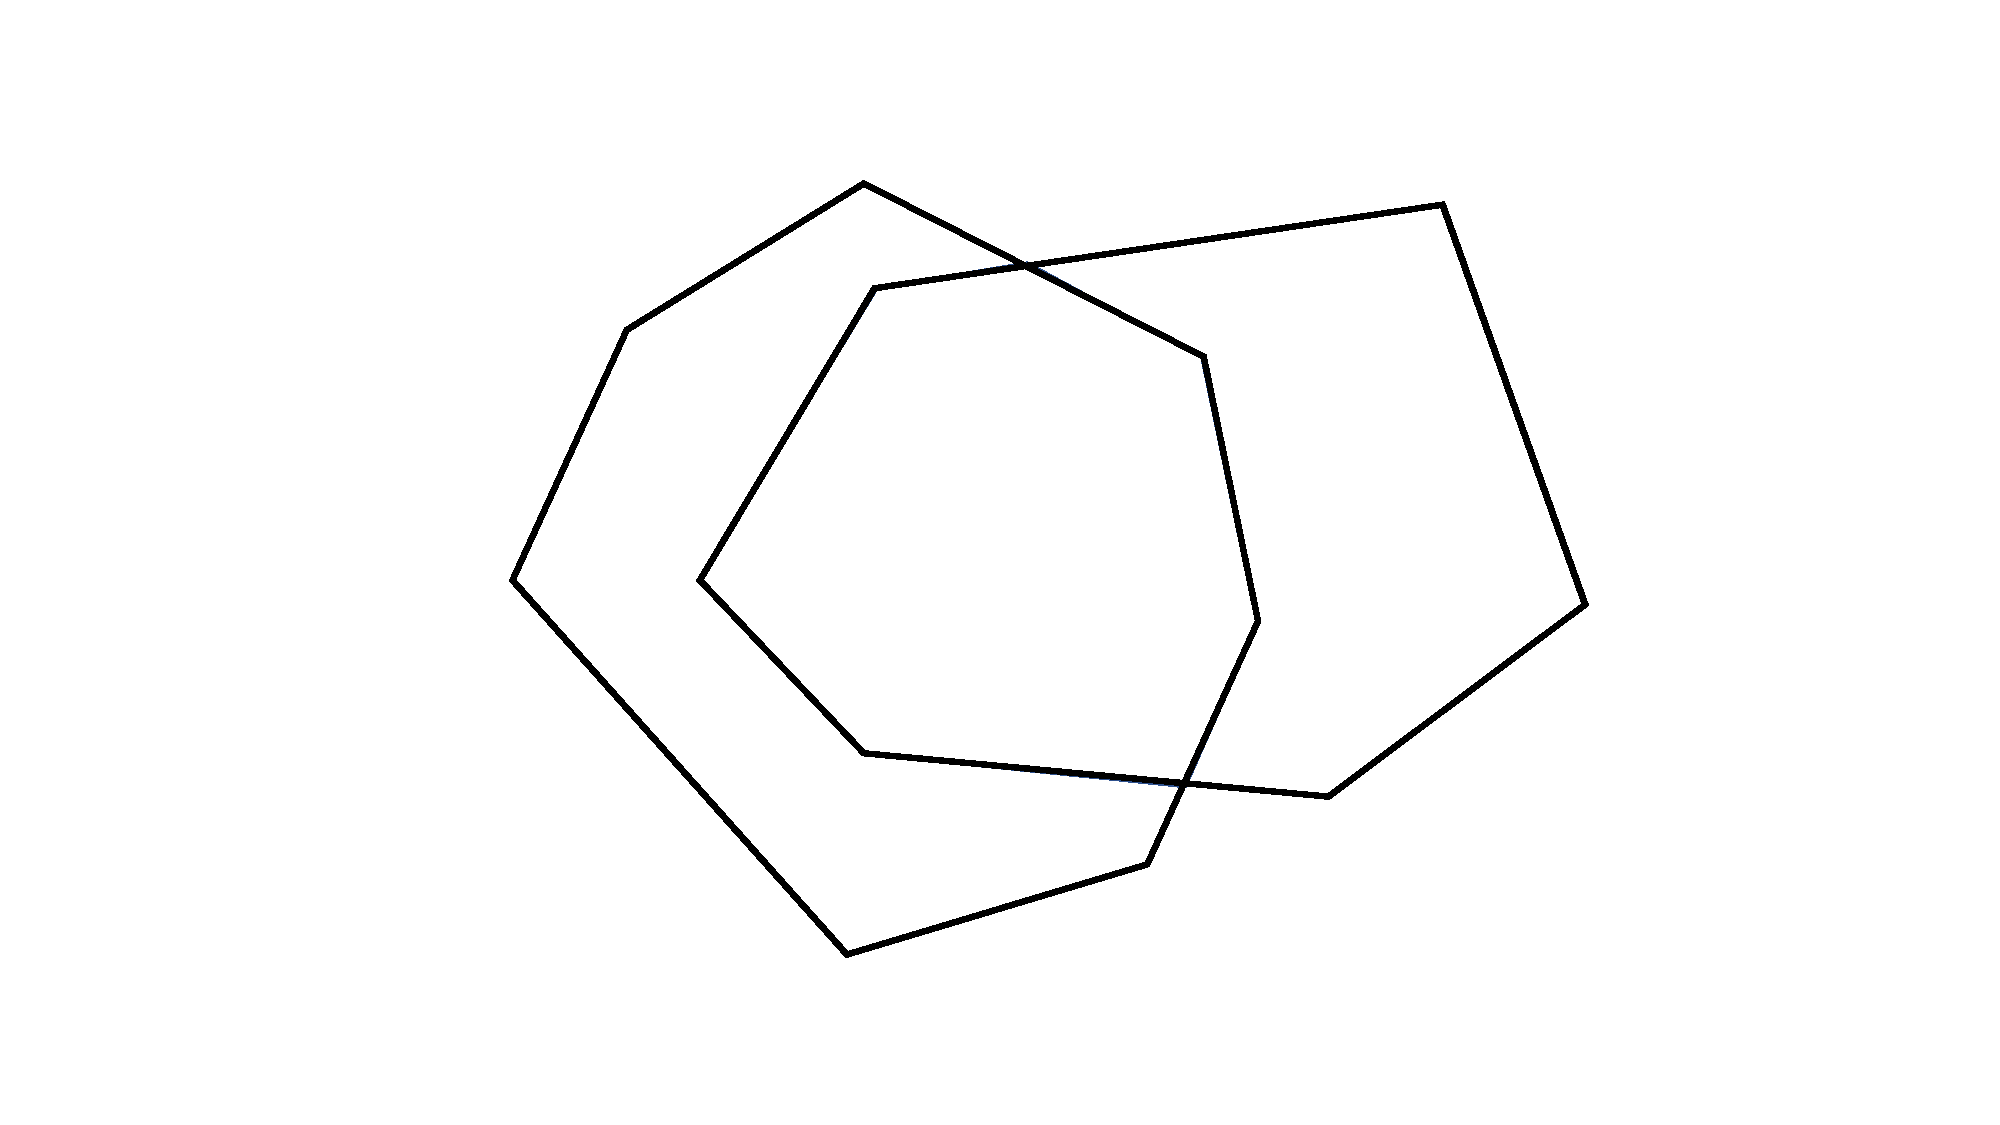
\includegraphics[width=0.3\linewidth]{../images/worksheet2b_no_color.pdf}

\vspace{25pt}
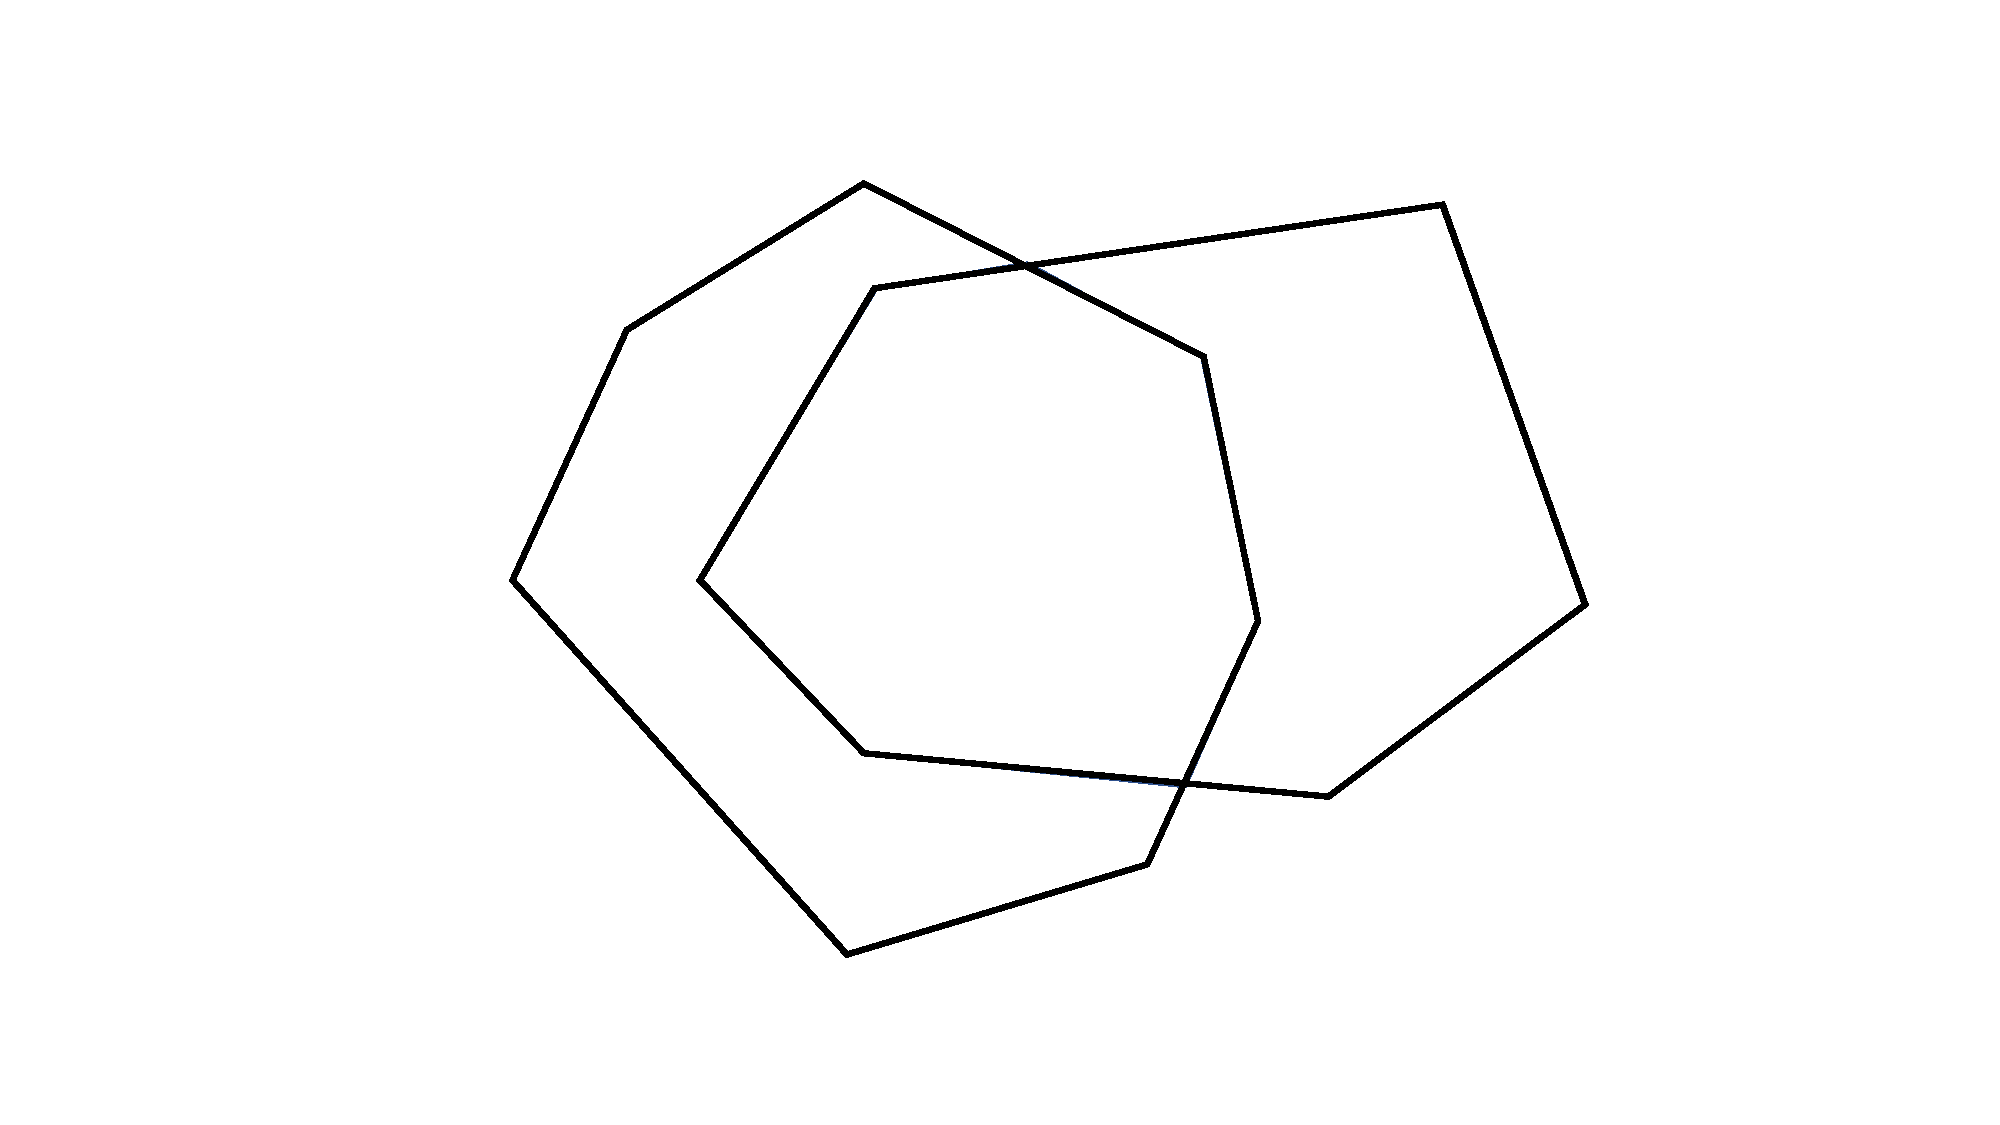
\includegraphics[width=0.3\linewidth]{../images/worksheet2b_no_color.pdf}\hfill
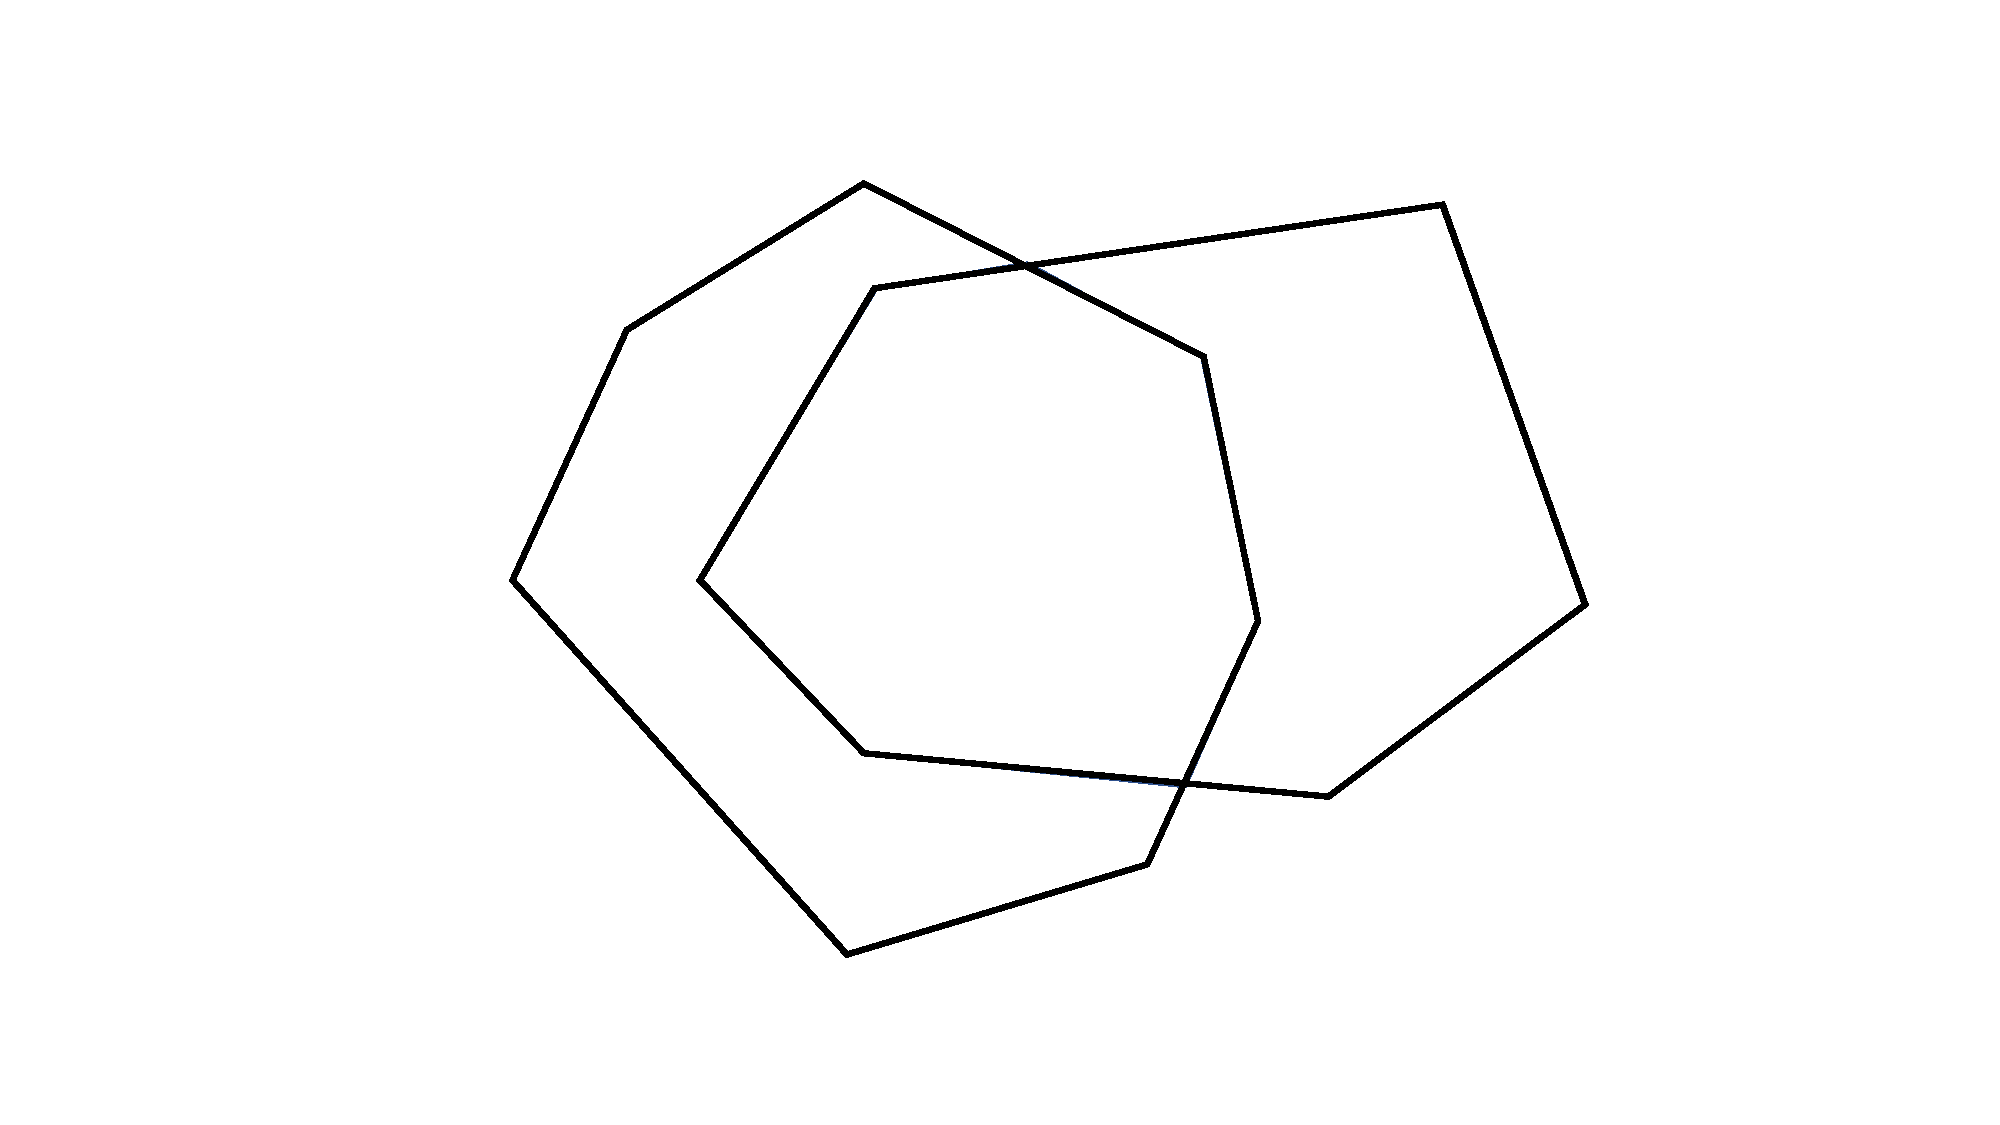
\includegraphics[width=0.3\linewidth]{../images/worksheet2b_no_color.pdf}\hfill
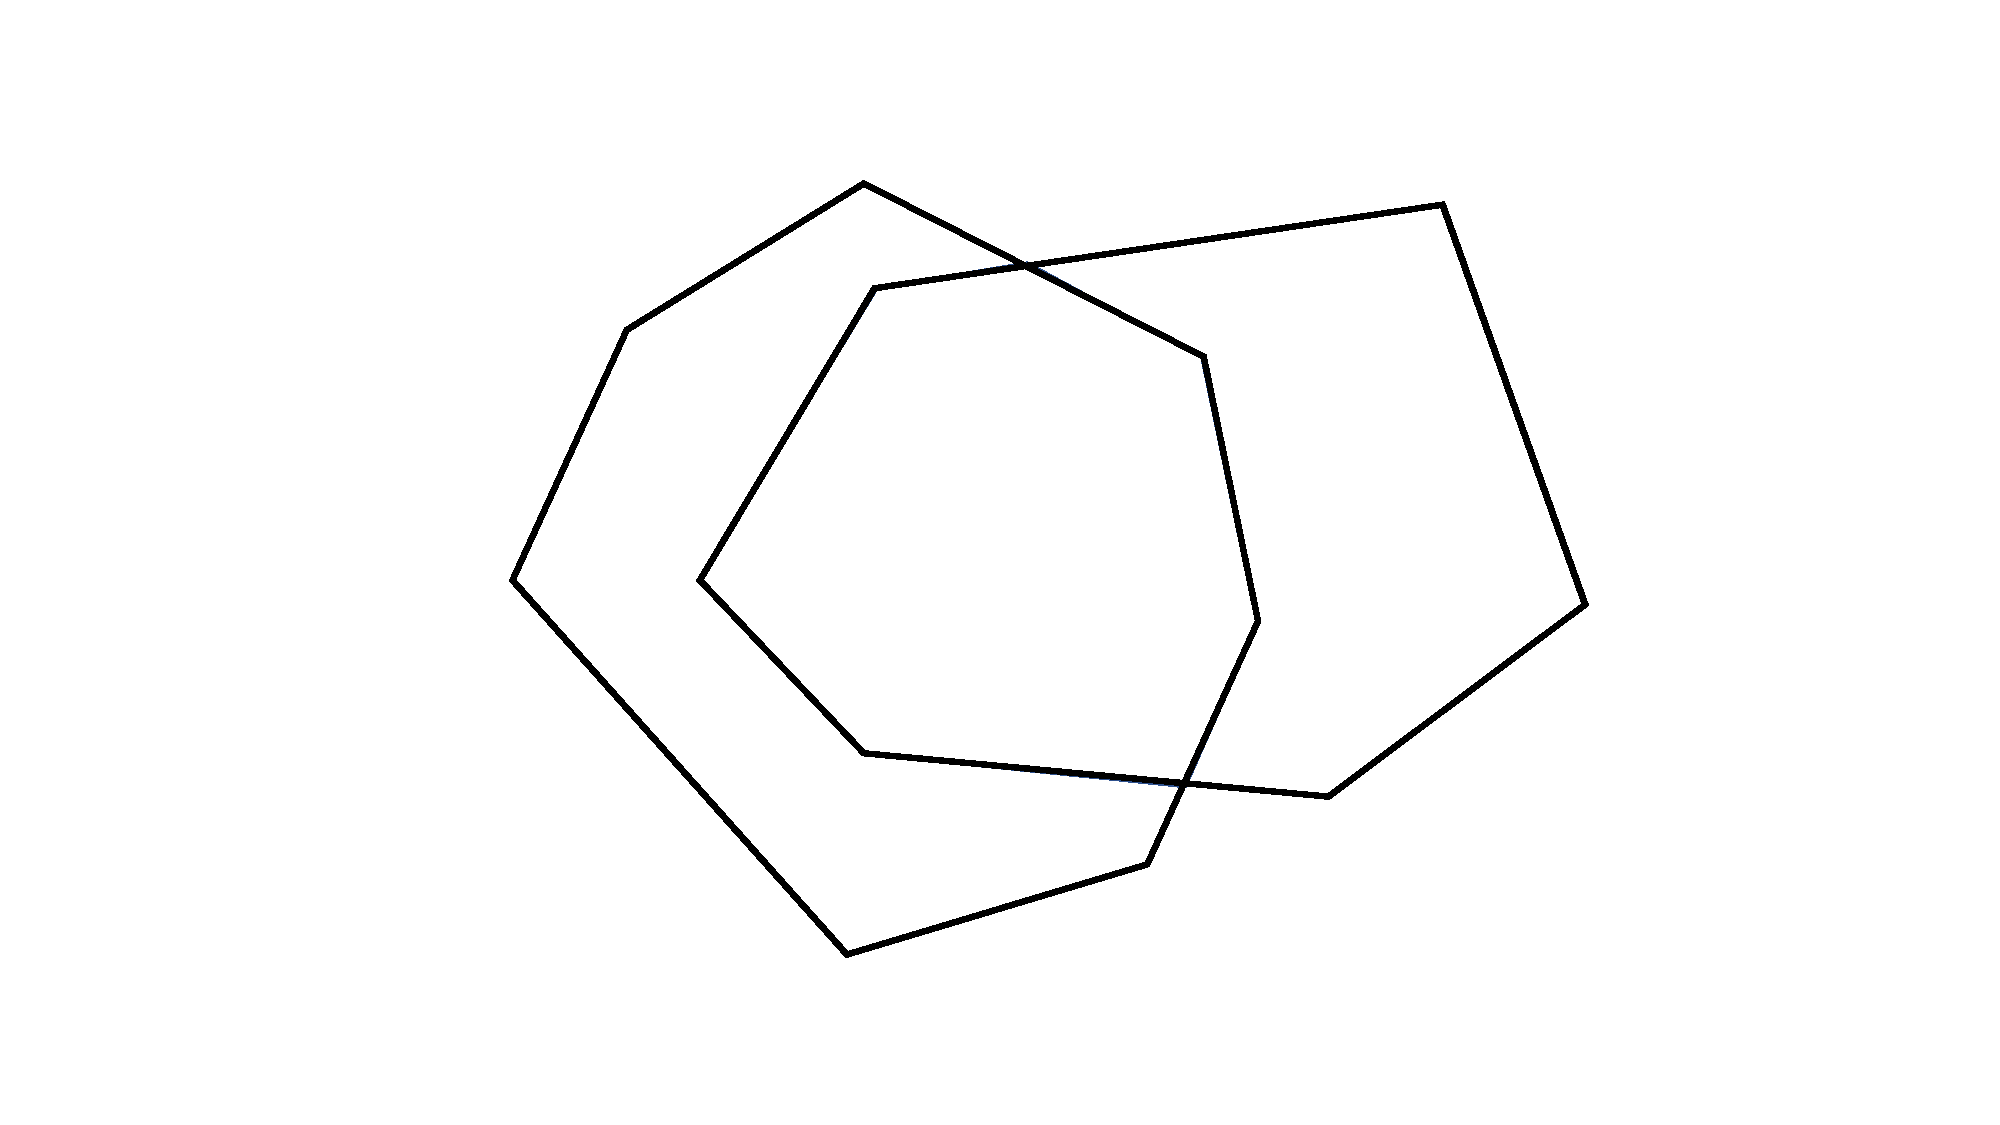
\includegraphics[width=0.3\linewidth]{../images/worksheet2b_no_color.pdf}

\vspace{25pt}
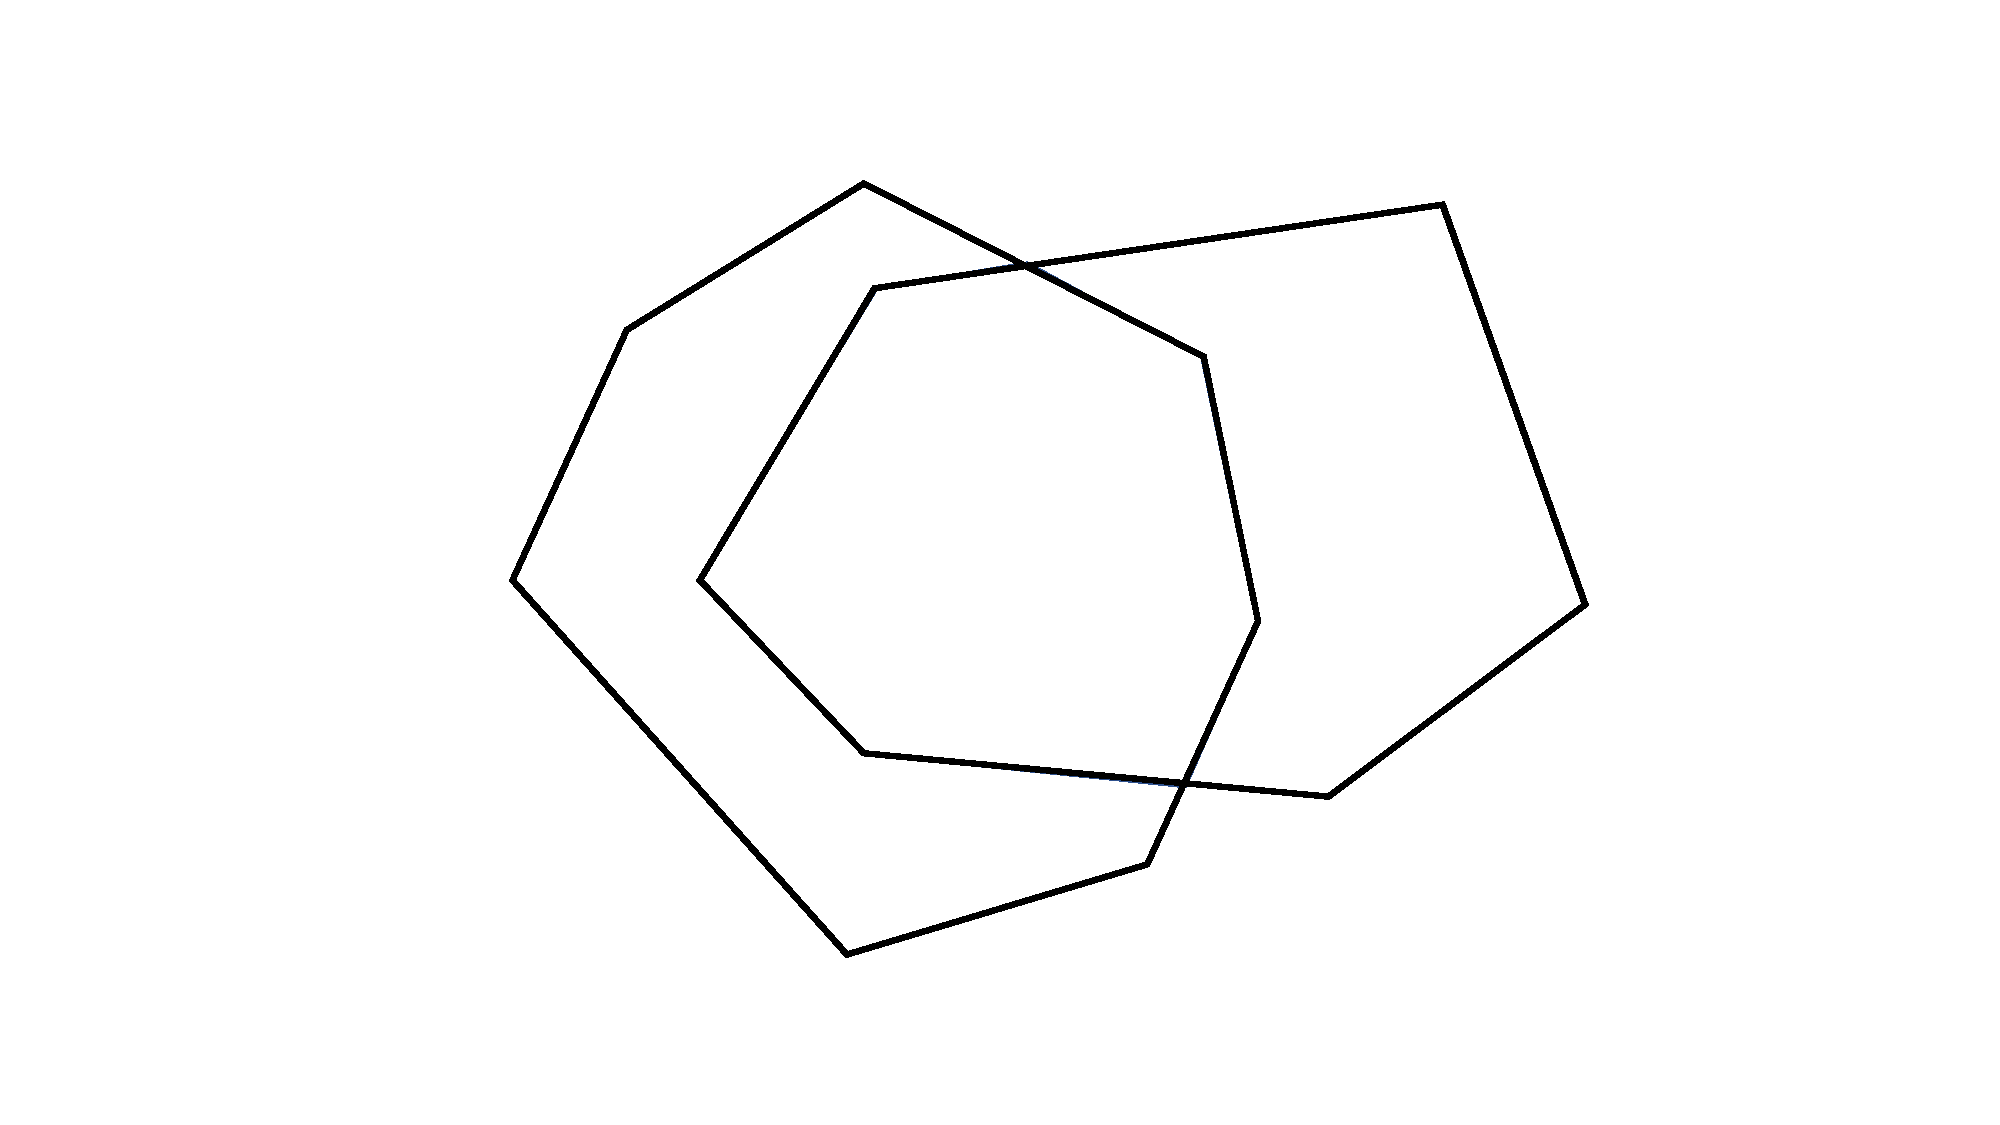
\includegraphics[width=0.3\linewidth]{../images/worksheet2b_no_color.pdf}\hfill
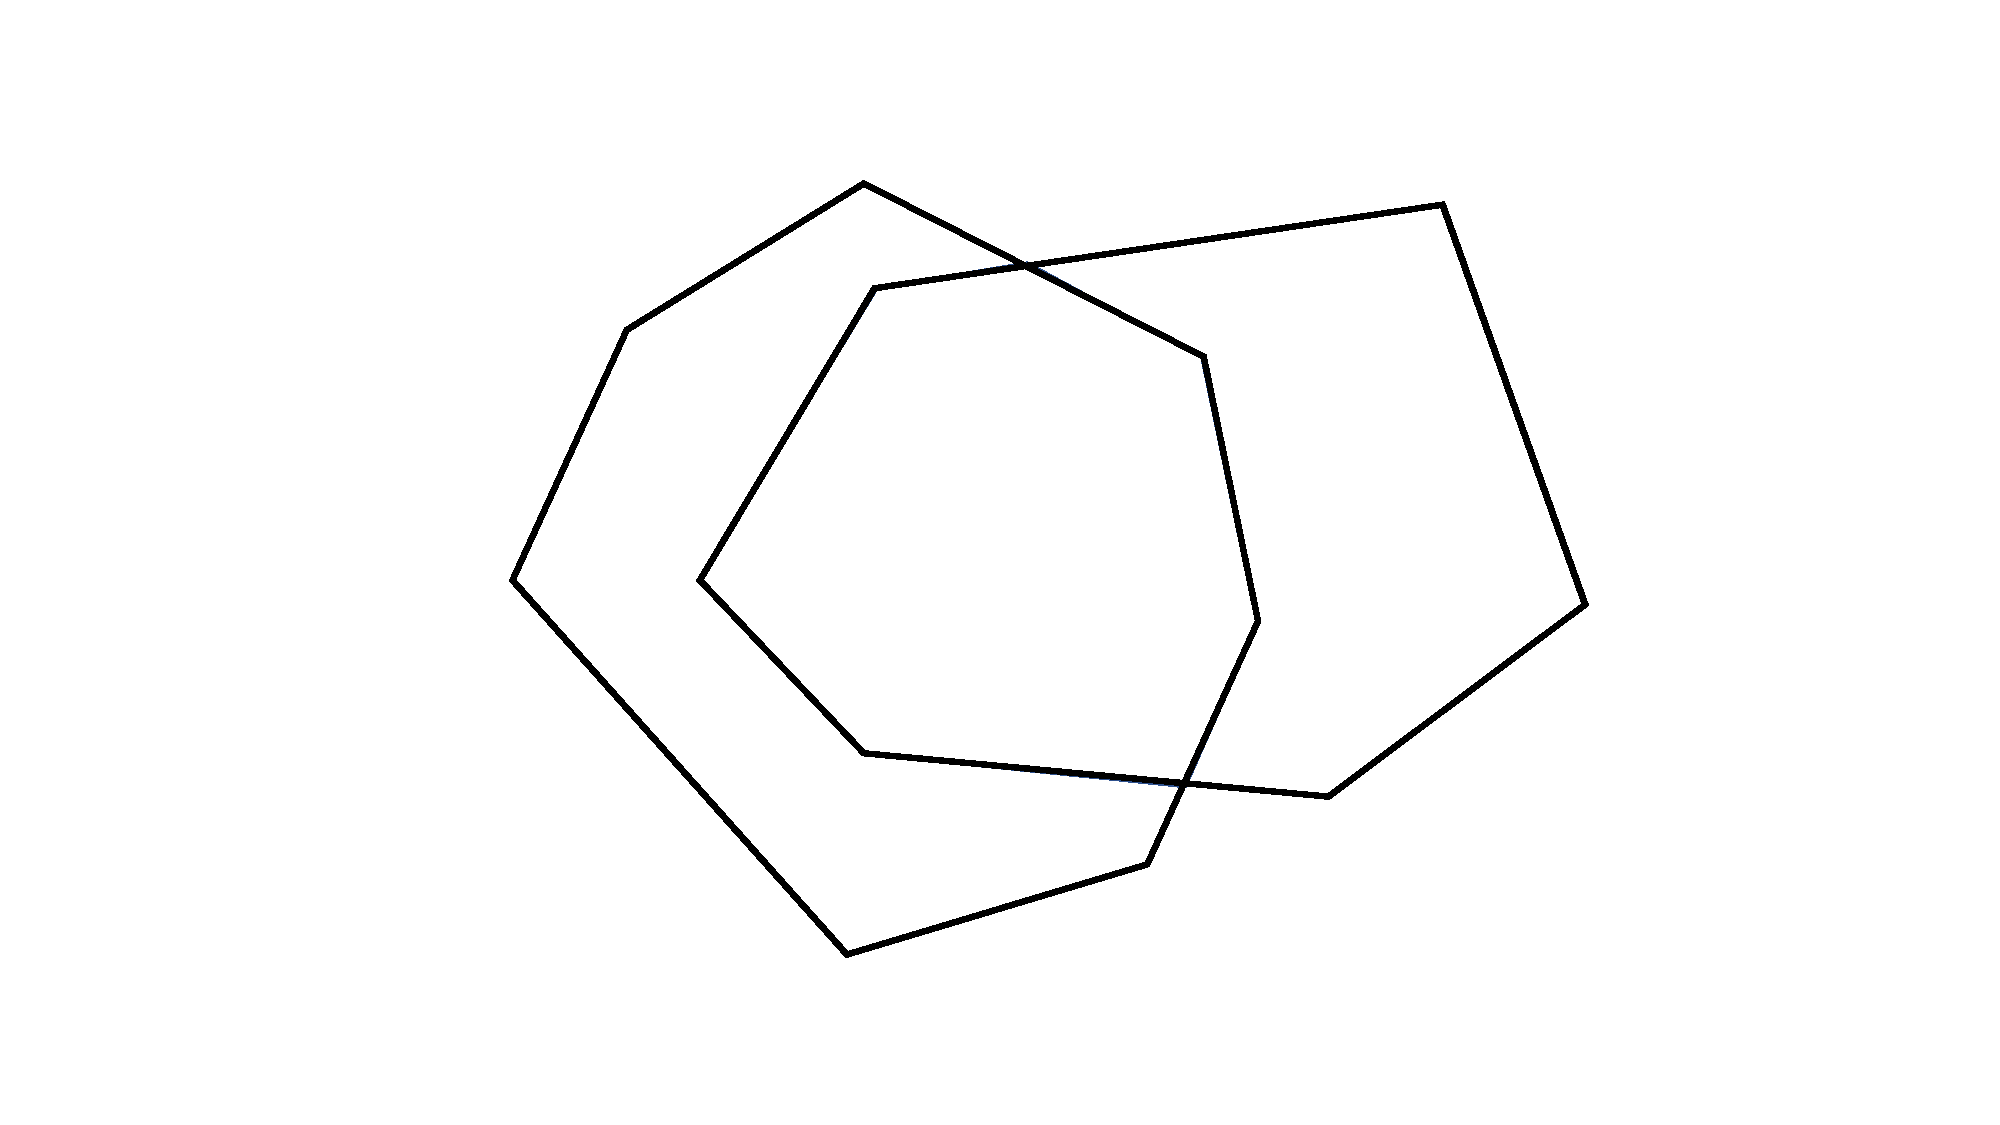
\includegraphics[width=0.3\linewidth]{../images/worksheet2b_no_color.pdf}\hfill
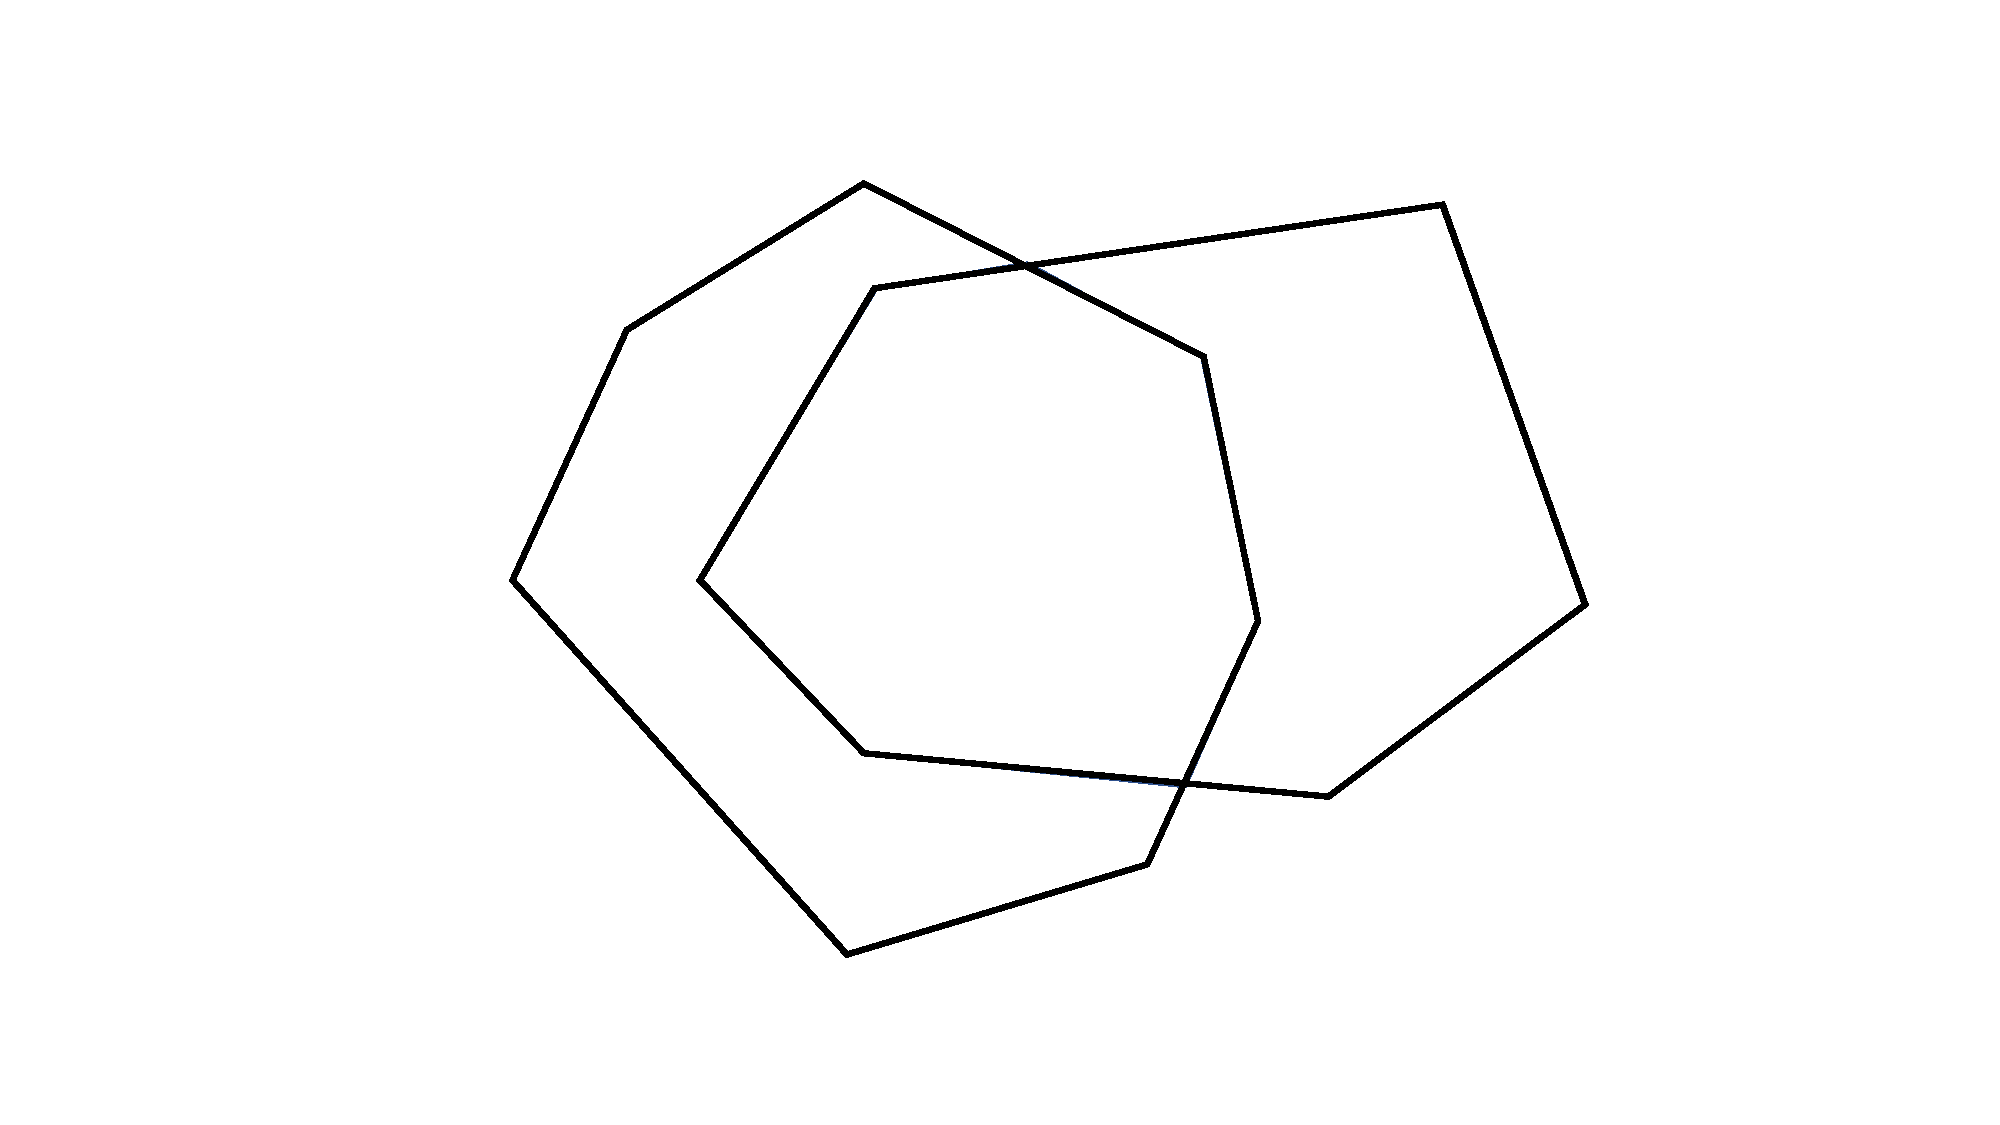
\includegraphics[width=0.3\linewidth]{../images/worksheet2b_no_color.pdf}

\end{document}

